\documentclass[11pt,a4paper]{article}

% ==============================================================================
% PAQUETES ESTÁNDAR (100% COMPATIBLE CON OVERLEAF Y PDFLATEX)
% ==============================================================================
\usepackage[utf8]{inputenc}
\usepackage[T1]{fontenc}
\usepackage[spanish,es-tabla,es-nodecimaldot]{babel}
\usepackage{lmodern}
\usepackage[left=2.4cm,right=2.4cm,top=2.4cm,bottom=2.4cm]{geometry}
\usepackage{setspace}
\usepackage{parskip}
\usepackage{graphicx}
\usepackage{adjustbox}
\usepackage{float}
\usepackage{amsmath,amssymb}
\usepackage{booktabs}
\usepackage{array}
\usepackage[table]{xcolor}
\usepackage{caption}
\usepackage{enumitem}
\usepackage[hidelinks]{hyperref}

% ==============================================================================
% ESTILO VISUAL LIMPIO BASADO EN TEMPLATE.PDF (SIN CÓDIGO EN EL INFORME)
% ==============================================================================
\definecolor{verdeHeader}{HTML}{548235}
\definecolor{verdeSuave}{HTML}{E2EFDA}
\definecolor{azulSuave}{HTML}{D6EAF8}
\definecolor{azulTitulo}{HTML}{1F4E79}

\hypersetup{
    colorlinks=true,
    linkcolor=azulTitulo,
    urlcolor=azulTitulo,
    citecolor=azulTitulo,
    pdftitle={Análisis Multiescala del Tejido Urbano en el Distrito de Puno}
}

\captionsetup{
    font=small,
    labelfont=bf,
    justification=justified,
    singlelinecheck=false
}

\onehalfspacing
\setlength{\parindent}{0.75cm}
\setlength{\parskip}{4pt}

% ==============================================================================
% INICIO DEL DOCUMENTO
% ==============================================================================
\begin{document}

% ------------------------------------------------------------------------------
% ENCABEZADO (ESTILO ARTÍCULO DE TEMPLATE.PDF)
% ------------------------------------------------------------------------------
\begin{center}
	{\Large \textbf{Análisis Multiescala del Tejido Urbano en el Distrito de Puno mediante Modelos de Árboles de Decisión}}\\[10pt]
	{\normalsize Apaza Quispe Royer / Diaz Tito Catherine Milagros}\\[4pt]
	{\small \textit{Curso: Estructuras de Datos Avanzadas (EDA) }}\\
	{\small \textit{Universidad Nacional del Altiplano — Puno, Perú}}\\[4pt]
\end{center}

\vspace{6pt}

\noindent\textbf{Resumen}

\noindent El presente informe desarrolla un análisis y modelado multiescala del espacio urbano del Distrito de Puno ($460.41\text{ km}^2$) utilizando datos cartográficos abiertos de OpenStreetMap (OSM) e integrando cuatro modelos basados en árboles de decisión y ensambles: \texttt{DecisionTreeClassifier} (criterios de Gini y Entropía), \texttt{RandomForestClassifier}, \texttt{XGBClassifier} (XGBoost) y \texttt{LGBMClassifier} (LightGBM). El trabajo se estructura de manera secuencial en cuatro etapas: Delimitación espacial y caracterización diagnóstica de los datos crudos de Puno, clasificación a Nivel Micro sobre $652$ edificaciones individuales, clasificación a Nivel Macro sobre una grilla regular de $250\text{ m} \times 250\text{ m}$ ($2{,}100$ celdas activas) y evaluación comparativa global, concordancia entre modelos y cartografía final integrada.

\noindent\textbf{Palabras clave:} Árboles de decisión, Ensambles, Random Forest, XGBoost, LightGBM, OpenStreetMap, Zonificación urbana, Puno.

\vspace{4pt}

\noindent\textbf{Abstract}

\noindent This report presents a supervised multiscale analysis and classification of the urban fabric of the Puno District ($460.41\text{ km}^2$, Peru) using OpenStreetMap (OSM) open geospatial data and comparing four tree-based machine learning models: \texttt{DecisionTreeClassifier} (Gini impurity and Shannon Entropy), \texttt{RandomForestClassifier}, \texttt{XGBClassifier} (XGBoost), and \texttt{LGBMClassifier} (LightGBM). The study follows four sequential stages: (1) spatial delimitation and raw data diagnosis for Puno, (2) Micro-level classification across $652$ individual buildings, (3) Macro-level urban zoning over a regular $250\text{ m} \times 250\text{ m}$ grid ($2{,}100$ active cells), and (4) global comparative evaluation, inter-model agreement, and integrated multiscale mapping.

\noindent\textbf{Keywords:} Decision trees, Ensemble learning, Random Forest, XGBoost, LightGBM, OpenStreetMap, Urban zoning, Puno.

\newpage

% ==============================================================================
% SECCIÓN 1: INTRODUCCIÓN Y OBJETIVOS
% ==============================================================================
\section{Introducción}
\label{sec:introduccion}

El crecimiento acelerado y heterogéneo de las ciudades intermedias andinas plantea desafíos constantes para la planificación territorial, la dotación de infraestructura pública y la gestión de servicios urbanos. En el caso del Distrito de Puno —ubicado a orillas del Lago Titicaca en el altiplano peruano, con una extensión de $460.41\text{ km}^2$. Frente a esta brecha, los repositorios abiertos de información geográfica voluntaria como OpenStreetMap (OSM) ofrecen una alternativa accesible y continua (Haklay \& Weber, 2008); sin embargo, su aprovechamiento analítico exige superar el elevado porcentaje de edificaciones y sectores territoriales que carecen de etiqueta funcional explícita.

En este contexto, los algoritmos supervisados basados en árboles de decisión y métodos de ensamble constituyen herramientas idóneas para modelar datos geoespaciales tabulares, pues capturan relaciones no lineales, combinan variables morfológicas con métricas espaciales y preservan mecanismos de interpretabilidad mediante reglas jerárquicas e importancia de atributos. Complementariamente, el uso de estructuras de datos espaciales avanzadas como el árbol $k$-dimensional (\texttt{cKDTree}; Bentley, 1975) permite calcular vecindades urbanas y distancias euclidianas en complejidad logarítmica $O(\log N)$, haciendo viable una caracterización territorial multiescala que conecte el comportamiento de cada edificación individual con la dinámica funcional de su entorno urbano y rural.

En consecuencia, el objetivo general del presente estudio es diseñar, implementar y evaluar comparativamente un flujo de clasificación supervisada multiescala del tejido urbano del Distrito de Puno utilizando datos vectoriales abiertos de OpenStreetMap y cuatro modelos basados en árboles de decisión y ensambles (\texttt{DecisionTreeClassifier}, \texttt{RandomForestClassifier}, \texttt{XGBClassifier} y \texttt{LGBMClassifier}). De manera específica, se busca delimitar y diagnosticar las capas cartográficas oficiales del distrito en proyección métrica \texttt{EPSG:32719}; construir e imputar modelos predictivos tanto a Nivel Micro como a Nivel Macro mediante ingeniería de variables espaciales con \texttt{cKDTree}; contrastar empíricamente los criterios de impureza de Gini y Entropía, la poda por profundidad máxima y el desempeño de los paradigmas de Bagging y Gradient Boosting bajo validación cruzada estratificada y evaluación en prueba independiente; y verificar finalmente la concordancia inter-modelo así como la coherencia territorial entre ambas escalas de análisis.
\newpage
% ==============================================================================
% SECCIÓN 2: DELIMITACIÓN ESPACIAL Y DESCRIPCIÓN DE DATOS (BASADO EN NB 01)
% ==============================================================================
\section{Delimitación Espacial y Descripción de Datos del Distrito de Puno}
\label{sec:delimitacion}

Esta sección documenta el origen de la información geográfica, el proceso técnico seguido para delimitar exclusivamente el Distrito de Puno y el diagnóstico exploratorio de los datos crudos antes de aplicar cualquier algoritmo de aprendizaje automático.

\subsection{Estructura de los Archivos Originales (\texttt{.shp}, \texttt{.dbf}, \texttt{.shx}, \texttt{.prj}, \texttt{.cpg}) y Conversión a \texttt{.geojson}}

Los datos cartográficos base fueron descargados del repositorio abierto de OpenStreetMap para todo el Perú (Geofabrik), conformando un volumen aproximado de $1.5\text{ GB}$ almacenado originalmente en la carpeta \texttt{Data/}. Estos archivos corresponden al formato estándar de Sistemas de Información Geográfica denominado \textbf{ESRI Shapefile}, el cual no guarda cada capa en un único archivo, sino que distribuye obligatoriamente la información en cinco extensiones complementarias e inseparables (Tabla~\ref{tab:shapefile}).

\begin{table}[H]
    \centering
    \caption{Descripción de las cinco extensiones del formato ESRI Shapefile presentes en los datos crudos.}
    \label{tab:shapefile}
    \small
    \begin{adjustbox}{max width=\textwidth}
    \begin{tabular}{llp{9.2cm}}
        \toprule
        \rowcolor{verdeHeader}
        \textcolor{white}{\textbf{Extensión}} & \textcolor{white}{\textbf{Función Principal}} & \textcolor{white}{\textbf{Contenido Almacenado}} \\
        \midrule
        \texttt{.shp} & \textit{Shape} (Geometrías) & Almacena las coordenadas vectoriales reales de cada polígono, línea o punto (huellas de edificios, calles, parques y lagos). \\
        \rowcolor{verdeSuave!50}
        \texttt{.dbf} & \textit{Database File} (Atributos) & Contiene la tabla descriptiva asociada a cada geometría, con campos como identificador (\texttt{osm\_id}), nombre (\texttt{name}), clase (\texttt{fclass}) y tipo (\texttt{type}). \\
        \texttt{.shx} & \textit{Shape Index} (Índice) & Índice posicional de acceso directo que enlaza cada geometría del archivo \texttt{.shp} con su fila exacta en la tabla \texttt{.dbf}. \\
        \rowcolor{verdeSuave!50}
        \texttt{.prj} & \textit{Projection} (Proyección) & Define el Sistema de Referencia de Coordenadas geográficas de la capa (\texttt{WGS 84 / EPSG:4326}). \\
        \texttt{.cpg} & \textit{Code Page} (Codificación) & Especifica la codificación de texto (\texttt{UTF-8}) necesaria para leer correctamente tildes y caracteres del español como la letra \textit{ñ}. \\
        \bottomrule
    \end{tabular}
    \end{adjustbox}
\end{table}

\textbf{¿Por qué se transforman a formato \texttt{.geojson}?} Trabajar directamente sobre los archivos Shapefile nacionales presenta tres desventajas prácticas: Requieren mantener cinco archivos sincronizados por cada capa, ocupan alrededor de $1.5\text{ GB}$ por incluir todo el territorio peruano y poseen limitaciones antiguas en nombres de columnas y portabilidad web. Al recortar exclusivamente el Distrito de Puno y exportar cada capa a \textbf{\texttt{.geojson}}, se logra unificar geometría, atributos y proyección en un solo archivo ligero basado en texto estructurado JSON. Como resultado, el conjunto completo de capas de Puno se reduce a apenas $3.53\text{ MB}$ descomprimidos, permitiendo una ejecución rápida, reproducible y totalmente compatible con herramientas de visualización web y Google Colab.

\subsection{Extracción del Límite Oficial del Distrito de Puno}

Para aislar el área de estudio se filtró el registro oficial correspondiente al \textbf{Distrito de Puno} (\texttt{name == 'Puno'} y \texttt{fclass == 'admin\_level8'}, identificador oficial \texttt{OSM ID: 1913513}).

Un aspecto cartográfico clave adoptado en todo el proyecto es la diferenciación explícita de dos Sistemas de Referencia de Coordenadas (CRS):
\begin{itemize}[leftmargin=0.8cm, itemsep=2pt]
    \item \textbf{\texttt{EPSG:4326} (WGS 84 en grados geográficos):} Es el sistema original de OpenStreetMap; se emplea para almacenamiento en \texttt{GeoJSON} y despliegue en mapas interactivos web.
    \item \textbf{\texttt{EPSG:32719} (WGS 84 / UTM Zona 19 Sur en metros):} Es la proyección métrica oficial para el sur del Perú. Resulta obligatoria para calcular superficies reales en $\text{m}^2$ o $\text{km}^2$ y distancias euclidianas en metros sin distorsión angular.
\end{itemize}

Al proyectar el contorno oficial a \texttt{EPSG:32719}, se determinó que el Distrito de Puno abarca una \textbf{superficie oficial de $460.41\text{ km}^2$} y un \textbf{perímetro de $118.30\text{ km}$}, tomando como centro urbano de referencia la \textbf{Plaza de Armas de Puno} (latitud $-15.8402$, longitud $-70.0280$).


\subsection{Inventario de Capas Crudas y Muestra Real de los Datos de Puno}

El proceso de delimitación produjo nueve capas vectoriales limpias, conformadas por el límite distrital, cuatro capas principales (edificaciones, uso de suelo, red vial y puntos de interés) y cuatro capas complementarias (POIs poligonales, transporte, cuerpos de agua y quebradas/ríos).

\begin{table}[H]
    \centering
    \caption{Inventario completo de las nueve capas vectoriales recortadas para el Distrito de Puno (\texttt{data\_puno/}).}
    \label{tab:inventario_puno}
    \setlength{\tabcolsep}{4pt}
    \footnotesize
    \begin{adjustbox}{max width=\textwidth}
    \begin{tabular}{lllcrl}
        \toprule
        \rowcolor{verdeHeader}
        \textcolor{white}{\textbf{Capa}} & \textcolor{white}{\textbf{Archivo GeoJSON}} & \textcolor{white}{\textbf{Geom.}} & \textcolor{white}{\textbf{Reg.}} & \textcolor{white}{\textbf{Métrica Espacial}} & \textcolor{white}{\textbf{Rol en el Proyecto}} \\
        \midrule
        Límite Distrital & \texttt{puno\_distrito\_boundary.geojson} & Polígono & 1 & $460.41\text{ km}^2$ & Máscara administrativa oficial \\
        \rowcolor{verdeSuave!50}
        Edificaciones (Micro) & \texttt{puno\_buildings.geojson} & Polígonos & 652 & $0.30\text{ km}^2$ constr. & Unidad de análisis — Nivel Micro \\
        Uso de Suelo (Macro) & \texttt{puno\_landuse.geojson} & Polígonos & 273 & $41.35\text{ km}^2$ cub. & Etiquetas base — Nivel Macro \\
        \rowcolor{verdeSuave!50}
        Red Vial & \texttt{puno\_roads.geojson} & Líneas & 4{,}276 & $1{,}114.2\text{ km}$ tot. & Accesibilidad y densidad vial \\
        POIs Puntuales & \texttt{puno\_pois.geojson} & Puntos & 935 & 64 categorías & Servicios/comercio (\texttt{cKDTree}) \\
        \rowcolor{verdeSuave!50}
        POIs Poligonales & \texttt{puno\_pois\_a.geojson} & Polígonos & 330 & 31 categorías & Equipamiento y áreas verdes \\
        Transporte & \texttt{puno\_transport.geojson} & Puntos & 48 & 5 tipos & Proximidad a paraderos (Macro) \\
        \rowcolor{verdeSuave!50}
        Cuerpos de Agua & \texttt{puno\_water\_a.geojson} & Polígonos & 9 & Lago Titicaca & Distancia al borde lacustre \\
        Quebradas y Ríos & \texttt{puno\_waterways.geojson} & Líneas & 30 & $39.7\text{ km}$ & Contexto hídrico y relieve \\
        \bottomrule
    \end{tabular}
    \end{adjustbox}
\end{table}

\begin{table}[H]
    \centering
    \caption{Muestra real de registros crudos en \texttt{puno\_buildings.geojson} (columnas originales de OSM).}
    \label{tab:crudo_buildings}
    \footnotesize
    \begin{adjustbox}{max width=\textwidth}
    \begin{tabular}{rclllc}
        \toprule
        \rowcolor{verdeHeader}
        \textcolor{white}{\textbf{osm\_id}} & \textcolor{white}{\textbf{code}} & \textcolor{white}{\textbf{fclass}} & \textcolor{white}{\textbf{name}} & \textcolor{white}{\textbf{type}} & \textcolor{white}{\textbf{Geometría}} \\
        \midrule
        225903400 & 1500 & \texttt{building} & Iglesia de San Juan & \texttt{church} & Polígono \\
        \rowcolor{verdeSuave!50}
        245233060 & 1500 & \texttt{building} & Terminal Terrestre de Puno & \texttt{NaN} & Polígono \\
        245233061 & 1500 & \texttt{building} & Mercado Central & \texttt{NaN} & Polígono \\
        \rowcolor{verdeSuave!50}
        255732549 & 1500 & \texttt{building} & Iglesia Bíblica Bautista & \texttt{NaN} & Polígono \\
        315213481 & 1500 & \texttt{building} & Condor & \texttt{NaN} & Polígono \\
        \bottomrule
    \end{tabular}
    \end{adjustbox}
\end{table}

\begin{table}[H]
    \centering
    \caption{Muestra real de registros crudos en \texttt{puno\_landuse.geojson} junto a su superficie proyectada en UTM 19S.}
    \label{tab:crudo_landuse}
    \footnotesize
    \begin{adjustbox}{max width=\textwidth}
    \begin{tabular}{rcllr}
        \toprule
        \rowcolor{verdeHeader}
        \textcolor{white}{\textbf{osm\_id}} & \textcolor{white}{\textbf{code}} & \textcolor{white}{\textbf{fclass}} & \textcolor{white}{\textbf{name}} & \textcolor{white}{\textbf{Área ($\text{m}^2$)}} \\
        \midrule
        23782585 & 7202 & \texttt{park} & Parque Pino & 1{,}934.7 \\
        \rowcolor{verdeSuave!50}
        123162130 & 7206 & \texttt{cemetery} & Cementerio Central de Laykakota & 14{,}341.3 \\
        189172773 & 7202 & \texttt{park} & Óvalo Ramón Castilla & 2{,}663.6 \\
        \rowcolor{verdeSuave!50}
        189172774 & 7202 & \texttt{park} & Dante Nava & 1{,}052.8 \\
        234953768 & 7202 & \texttt{park} & \texttt{NaN} & 1{,}471.8 \\
        \bottomrule
    \end{tabular}
    \end{adjustbox}
\end{table}


\subsection{Ficha Visual de Nuestras Bases de Datos de Modelado (Nivel Micro y Nivel Macro)}

El proyecto articula dos escalas complementarias con dimensiones claramente definidas:

\begin{figure}[H]
    \centering
    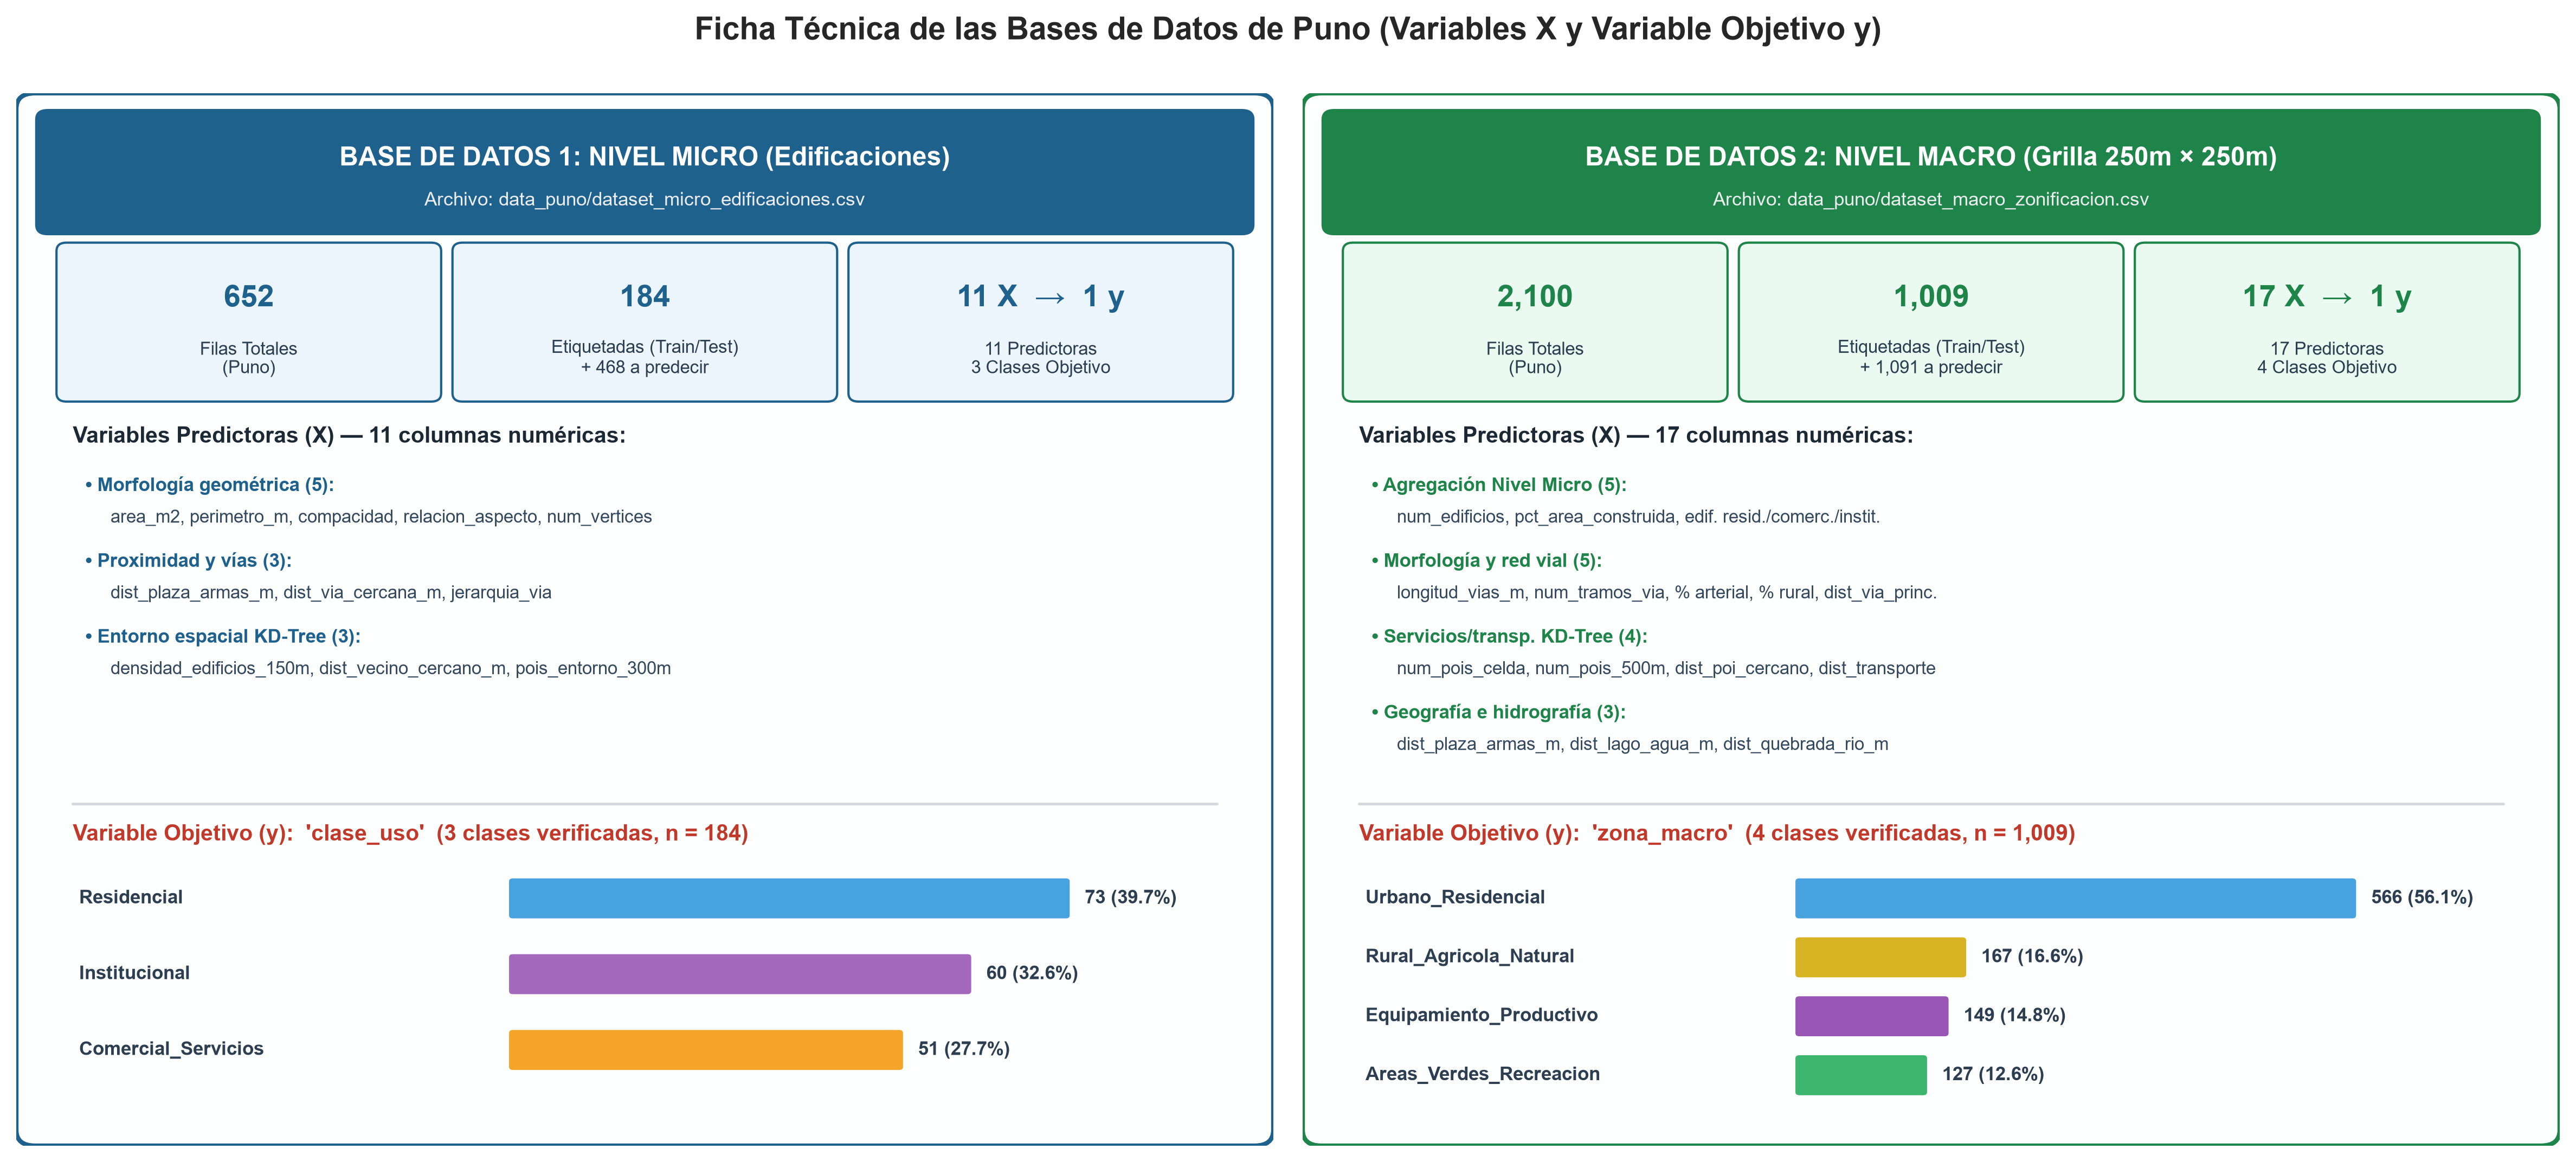
\includegraphics[width=0.99\textwidth]{figures/01_esquema_datasets_puno.png}
    \caption{Ficha técnica visual de las dos bases de datos de modelado de Puno: comparación de filas totales, registros etiquetados frente a registros por predecir, agrupación de variables predictoras ($X$) y distribución de clases de la variable objetivo ($y$).}
    \label{fig:ficha_datasets}
\end{figure}

A continuación, las Tablas~\ref{tab:muestra_micro_real} y~\ref{tab:muestra_macro_real} muestran ejemplos reales de ambas bases de datos tabulares de Puno, destacando con sombreado la columna correspondiente a la variable objetivo ($y$).

\begin{table}[H]
    \centering
    \caption{Ejemplos reales de filas etiquetadas del dataset Nivel Micro.}
    \label{tab:muestra_micro_real}
    \setlength{\tabcolsep}{4pt}
    \footnotesize
    \begin{adjustbox}{max width=\textwidth}
    \begin{tabular}{lrrrrrrrc}
        \toprule
        \rowcolor{verdeHeader}
        \textcolor{white}{\textbf{Edificio}} & \textcolor{white}{\textbf{Área ($\text{m}^2$)}} & \textcolor{white}{\textbf{Perím.}} & \textcolor{white}{\textbf{Comp.}} & \textcolor{white}{\textbf{D. Plaza}} & \textcolor{white}{\textbf{D. Vía}} & \textcolor{white}{\textbf{Dens. 150m}} & \textcolor{white}{\textbf{POIs 300m}} & \textcolor{white}{\textbf{clase\_uso ($y$)}} \\
        \midrule
        Iglesia de San Juan & 1{,}249.99 & 205.46 & 0.37 & 268.81 & 6.02 & 1 & 193 & \cellcolor{verdeSuave}\textbf{Institucional} \\
        Terminal Terrestre & 3{,}293.20 & 401.51 & 0.26 & 1{,}227.39 & 5.53 & 11 & 18 & \cellcolor{verdeSuave}\textbf{Comercial\_Serv.} \\
        Mercado Central & 2{,}858.43 & 223.21 & 0.72 & 338.44 & 3.09 & 4 & 200 & \cellcolor{verdeSuave}\textbf{Comercial\_Serv.} \\
        Iglesia Bíb. Bautista & 834.88 & 134.30 & 0.58 & 1{,}024.28 & 3.08 & 2 & 34 & \cellcolor{verdeSuave}\textbf{Institucional} \\
        Sin nombre (vivienda) & 96.95 & 40.85 & 0.73 & 924.61 & 4.03 & 21 & 21 & \cellcolor{verdeSuave}\textbf{Residencial} \\
        Sin nombre (vivienda) & 86.67 & 37.79 & 0.76 & 926.82 & 4.33 & 23 & 23 & \cellcolor{verdeSuave}\textbf{Residencial} \\
        \bottomrule
    \end{tabular}
    \end{adjustbox}
\end{table}

\begin{table}[H]
    \centering
    \caption{Ejemplos reales de filas etiquetadas del dataset Nivel Macro.}
    \label{tab:muestra_macro_real}
    \setlength{\tabcolsep}{4pt}
    \footnotesize
    \begin{adjustbox}{max width=\textwidth}
    \begin{tabular}{crrrrrrrc}
        \toprule
        \rowcolor{verdeHeader}
        \textcolor{white}{\textbf{cell\_id}} & \textcolor{white}{\textbf{Edif.}} & \textcolor{white}{\textbf{\% Constr.}} & \textcolor{white}{\textbf{Vías (m)}} & \textcolor{white}{\textbf{\% Art.}} & \textcolor{white}{\textbf{POIs 500m}} & \textcolor{white}{\textbf{D. Plaza}} & \textcolor{white}{\textbf{D. Lago}} & \textcolor{white}{\textbf{zona\_macro ($y$)}} \\
        \midrule
        3223 & 0 & 0.00 & 308.23 & 0.87 & 0 & 6{,}144.51 & 6{,}961.38 & \cellcolor{azulSuave}\textbf{Urbano\_Residencial} \\
        3322 & 0 & 0.00 & 30.40 & 0.00 & 0 & 5{,}653.90 & 6{,}618.90 & \cellcolor{azulSuave}\textbf{Urbano\_Residencial} \\
        3792 & 0 & 0.00 & 0.00 & 0.00 & 0 & 7{,}621.97 & 7{,}972.07 & \cellcolor{azulSuave}\textbf{Equip.\_Productivo} \\
        3793 & 0 & 0.00 & 0.00 & 0.00 & 0 & 7{,}417.36 & 7{,}808.79 & \cellcolor{azulSuave}\textbf{Equip.\_Productivo} \\
        4296 & 0 & 0.00 & 0.00 & 0.00 & 0 & 3{,}519.22 & 4{,}211.83 & \cellcolor{azulSuave}\textbf{Rural\_Agric.\_Nat.} \\
        4385 & 0 & 0.00 & 504.91 & 0.00 & 1 & 3{,}303.39 & 3{,}967.65 & \cellcolor{azulSuave}\textbf{Rural\_Agric.\_Nat.} \\
        4464 & 0 & 0.00 & 191.38 & 0.00 & 0 & 2{,}623.96 & 3{,}836.98 & \cellcolor{azulSuave}\textbf{Areas\_Verdes\_Rec.} \\
        4474 & 0 & 0.00 & 1{,}636.58 & 0.00 & 5 & 3{,}238.46 & 3{,}790.86 & \cellcolor{azulSuave}\textbf{Areas\_Verdes\_Rec.} \\
        \bottomrule
    \end{tabular}
    \end{adjustbox}
\end{table}

\subsection{Radiografía Descriptiva de los Datos Crudos de Puno (OpenStreetMap)}

Antes de entrenar los modelos predictivos, se elaboró una radiografía estadística de las cuatro capas principales recortadas para Puno (Figura~\ref{fig:radiografia_cruda}), la cual permite diagnosticar la calidad real de la información disponible en OpenStreetMap.

\begin{figure}[H]
    \centering
    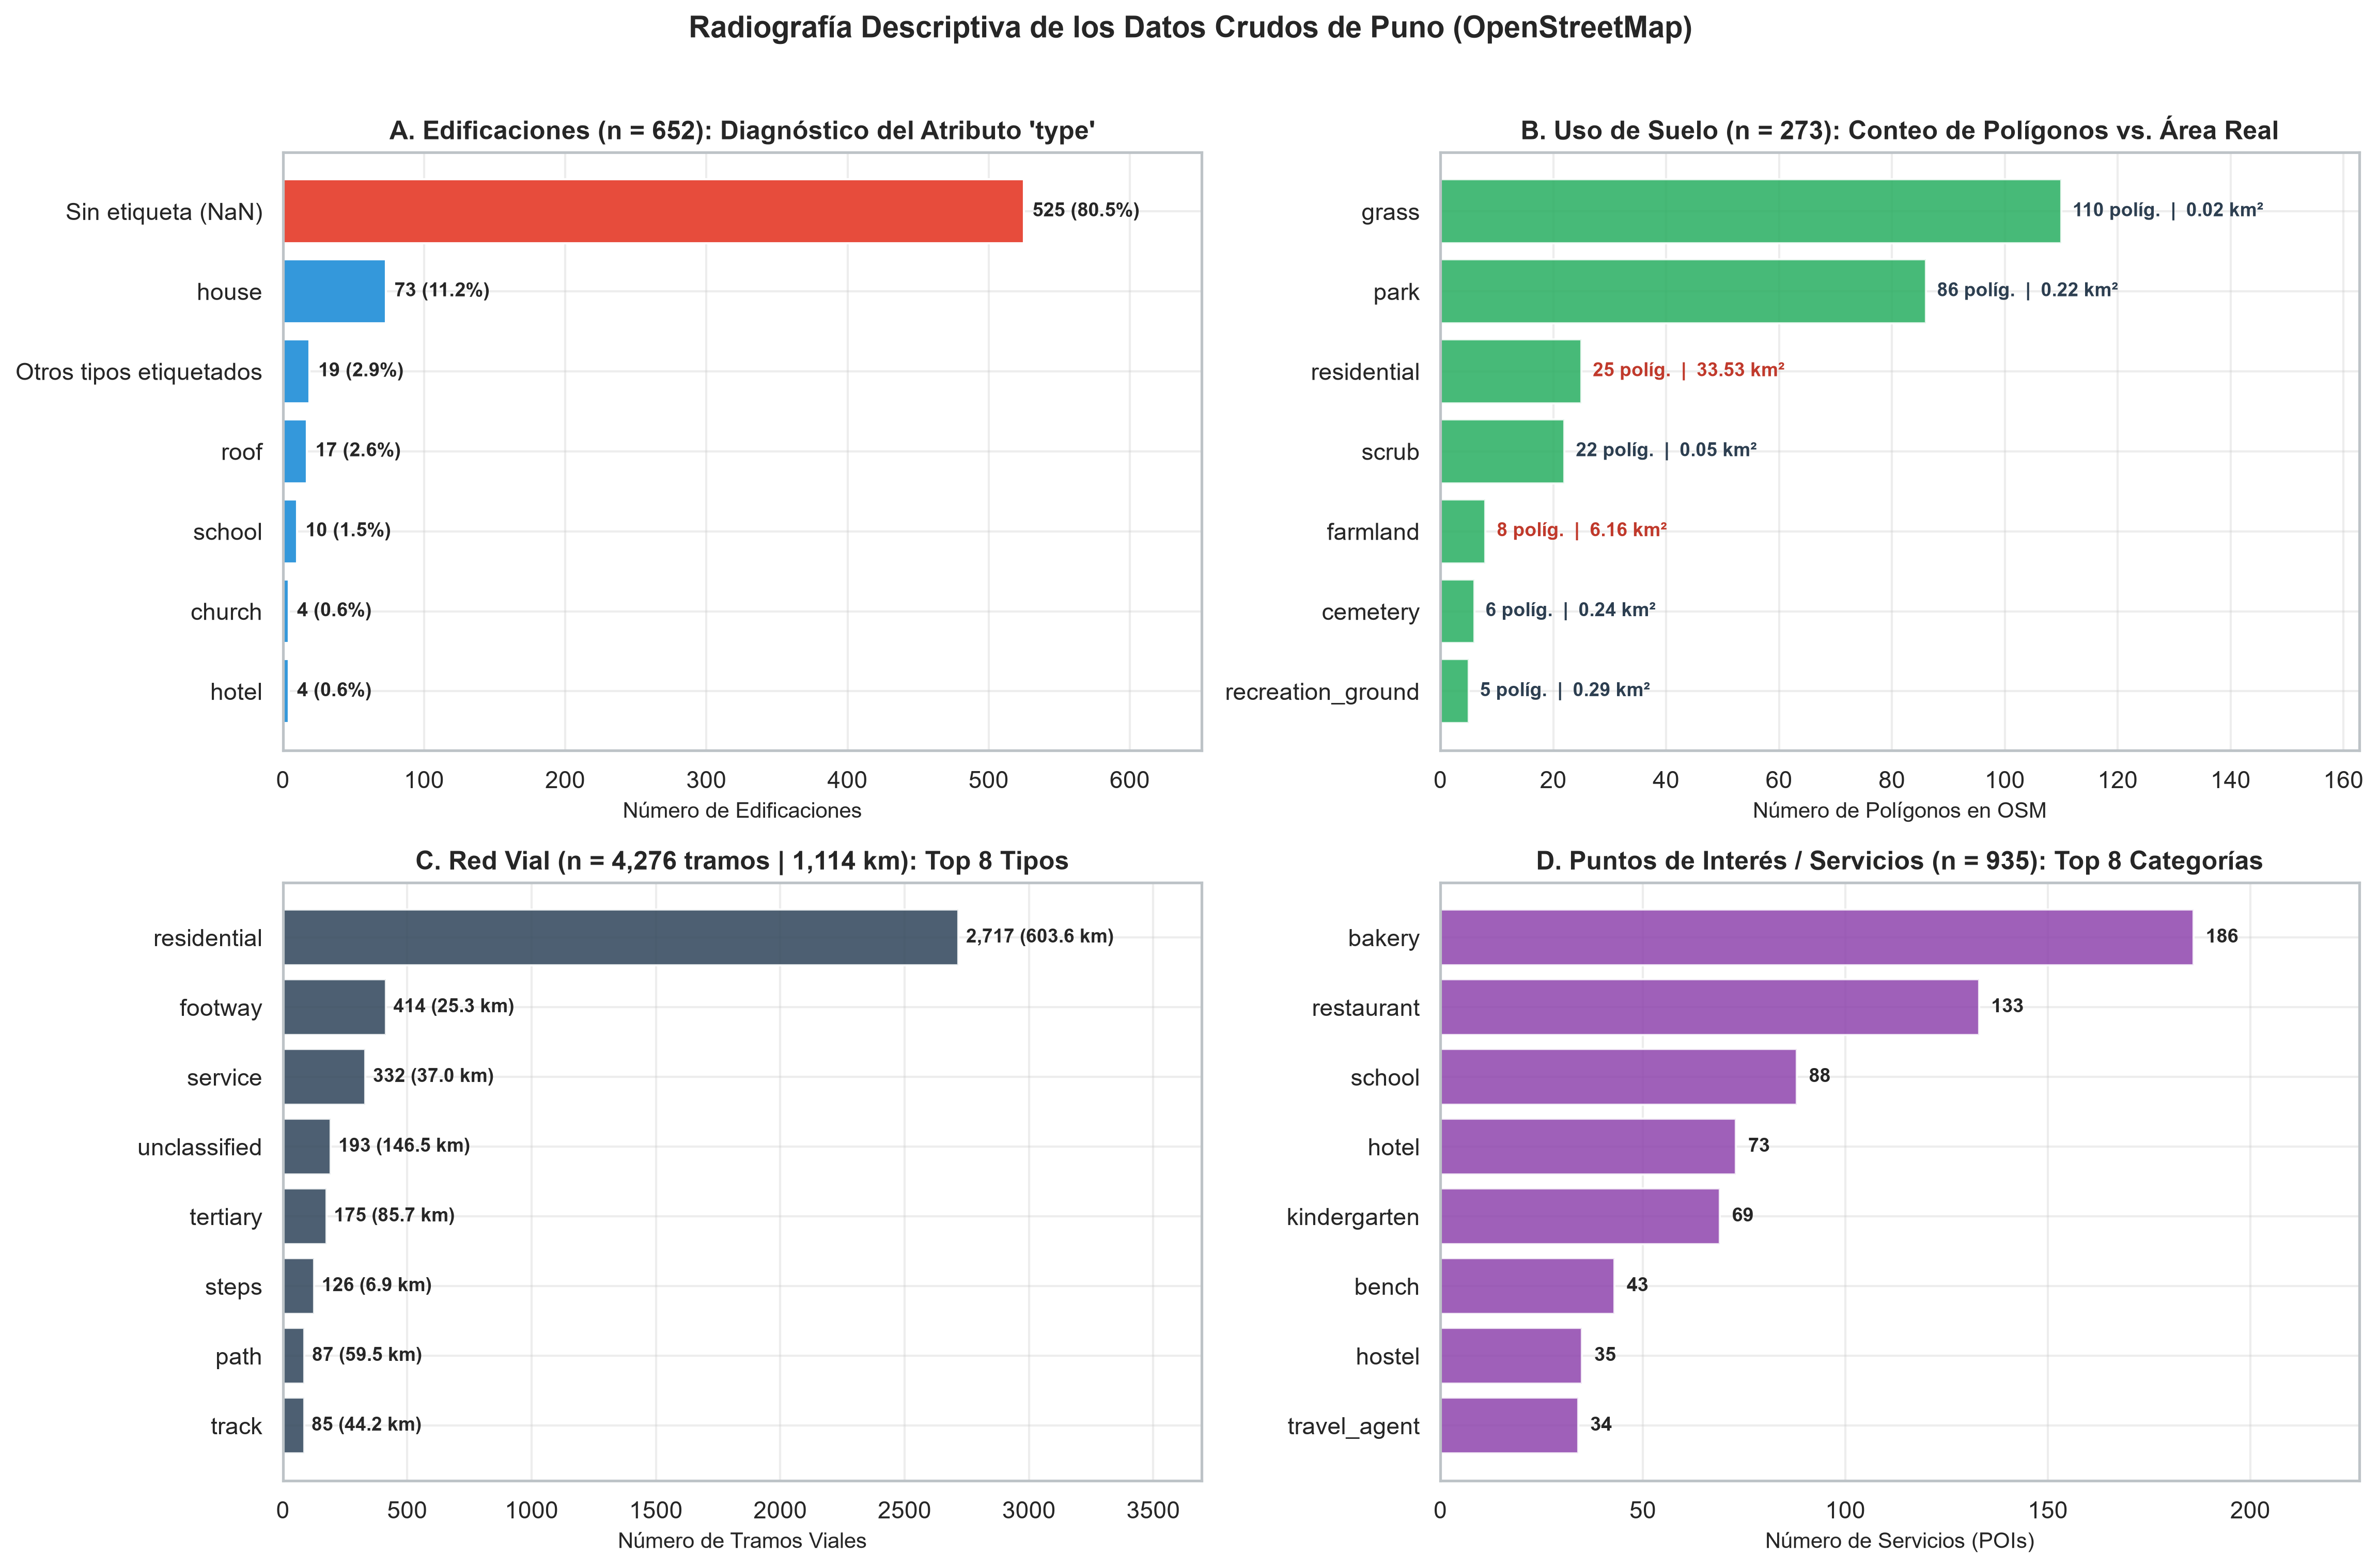
\includegraphics[width=0.98\textwidth]{figures/01_radiografia_datos_puno.png}
    \caption{Radiografía descriptiva de los datos crudos de OpenStreetMap en el Distrito de Puno: (A) diagnóstico de etiquetas en edificaciones, (B) conteo de polígonos frente a superficie real en uso de suelo, (C) distribución de tipos y kilómetros de la red vial, y (D) principales categorías de puntos de interés (POIs).}
    \label{fig:radiografia_cruda}
\end{figure}

\subsection{Visualización Cartográfica del Área de Estudio (Datos Crudos Recortados)}

Finalmente, la Figura~\ref{fig:mapa_crudo_puno} presenta la distribución espacial real de los datos crudos recortados para el Distrito de Puno en coordenadas métricas UTM Zona 19 Sur, antes de efectuar cualquier predicción o clasificación con algoritmos de aprendizaje automático.

\begin{figure}[H]
    \centering
    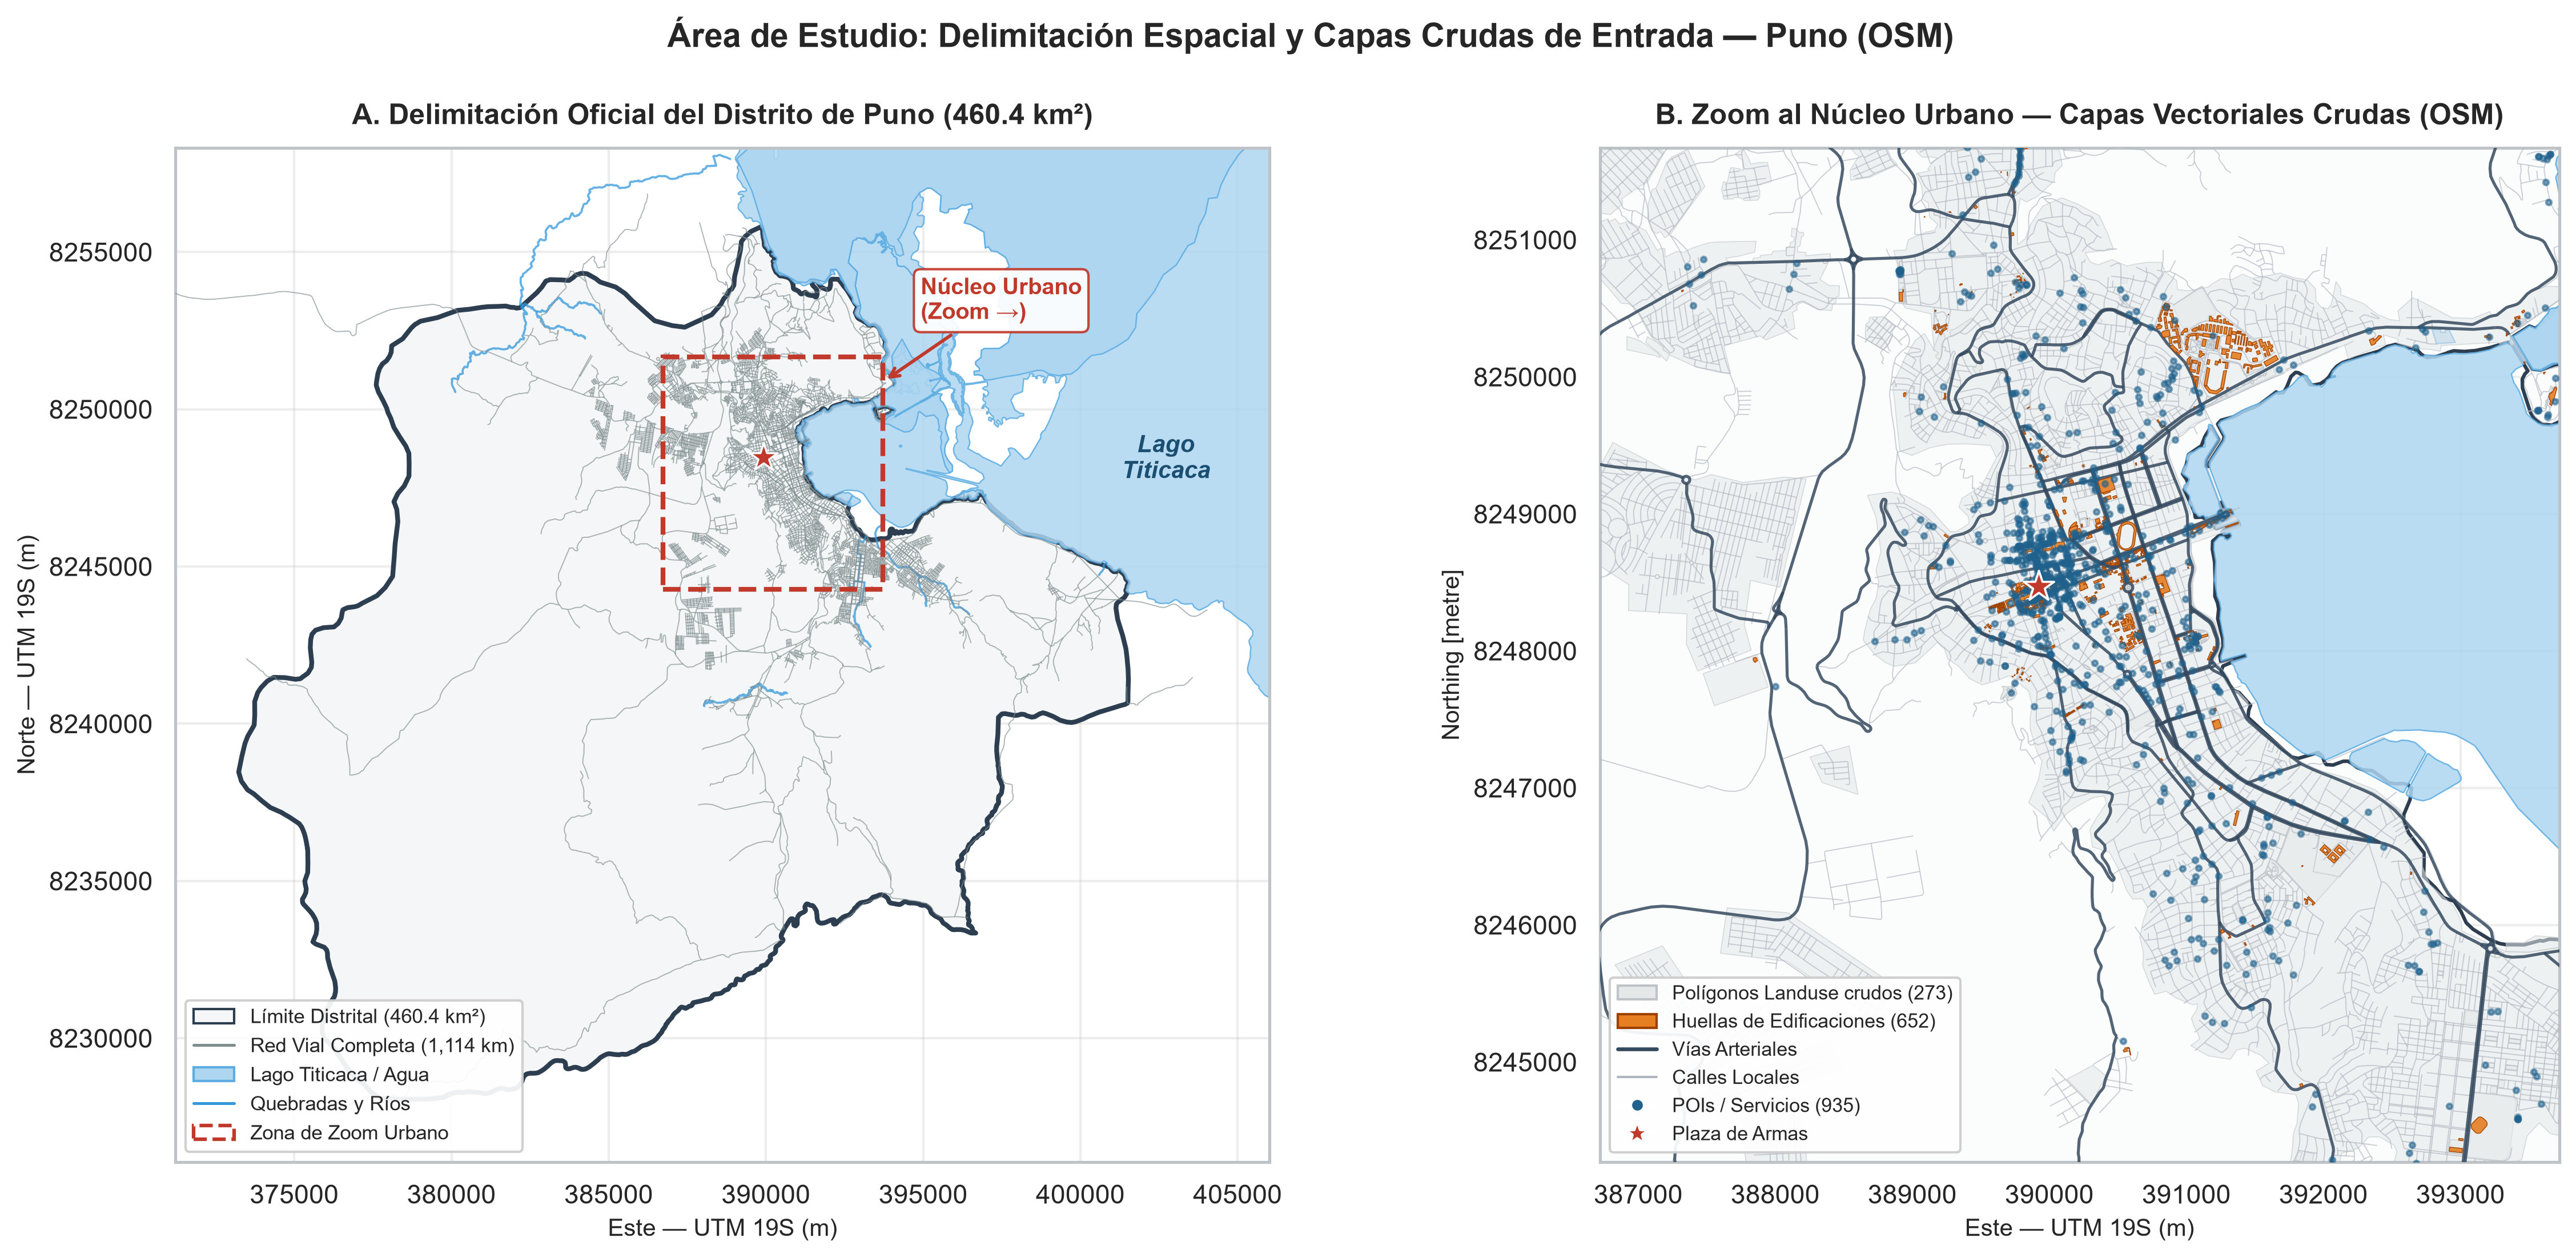
\includegraphics[width=0.99\textwidth]{figures/01_mapa_cartografico_puno.png}
    \caption{Visualización cartográfica de los datos crudos recortados para el Distrito de Puno: (A) contexto distrital completo ($460.4\text{ km}^2$) delimitado junto a la bahía del Lago Titicaca y (B) acercamiento al núcleo urbano mostrando la superposición espacial cruda de polígonos \texttt{landuse}, huellas de edificaciones, red vial jerarquizada y POIs.}
    \label{fig:mapa_crudo_puno}
\end{figure}


% ==============================================================================
% SECCIÓN 2: NIVEL MICRO — CLASIFICACIÓN DE EDIFICACIONES (BASADO EN NB 02)
% ==============================================================================
\section{Nivel Micro: Clasificación de Edificaciones en el Distrito de Puno}
\label{sec:micro}

Esta sección aborda el modelado supervisado a escala individual de lote o edificación (\textbf{Nivel Micro}). El propósito es aprovechar la geometría y el contexto urbano de las $652$ edificaciones digitalizadas en OpenStreetMap para entrenar, comparar e interpretar los cuatro modelos basados en árboles y finalmente imputar la función urbana de las $468$ edificaciones sin etiqueta.

\subsection{Construcción de la Variable Objetivo ($y$): Etiquetado Verificable}

Como se comprobó en la radiografía de datos de la Sección~\ref{sec:delimitacion}, solo $127$ edificaciones poseen el campo \texttt{type} en OpenStreetMap. Sin embargo, al auditar los atributos complementarios se identificaron edificaciones con nombre oficial explícito en \texttt{name} (por ejemplo, \textit{Mercado Central}, \textit{Terminal Terrestre de Puno}, \textit{Iglesia de San Juan}, \textit{Municipalidad}) y otras que contienen un Punto de Interés (POI) ubicado geométricamente dentro de su polígono (\texttt{hotel}, \texttt{restaurant}, \texttt{school}, \texttt{bank}, \texttt{hospital}).

Integrando estas tres señales verificables con reglas transparentes y sin ambigüedad, se consolidaron \textbf{$184$ edificaciones verificadas} agrupadas en \textbf{tres clases urbanas equilibradas}:
\begin{enumerate}[leftmargin=0.85cm, itemsep=2pt]
    \item \textbf{\texttt{Residencial} ($73$ edificaciones; $39.7\%$):} Viviendas familiares (\texttt{house}).
    \item \textbf{\texttt{Institucional} ($60$ edificaciones; $32.6\%$):} Colegios, facultades universitarias, hospitales, clínicas, iglesias, comisarías, municipalidad, gobierno regional, bomberos y estadios.
    \item \textbf{\texttt{Comercial\_Servicios} ($51$ edificaciones; $27.7\%$):} Hoteles, hostales, restaurantes, mercados, bancos, comercios minoristas, almacenes y terminal terrestre.
\end{enumerate}

Las \textbf{$468$ edificaciones restantes} (nulas o con etiquetas estructurales ambiguas como \texttt{roof} o \texttt{shed}) se mantuvieron sin etiqueta (\texttt{NaN}) para ser clasificadas al final mediante el modelo ganador. La Figura~\ref{fig:dist_micro} muestra la distribución de las tres clases verificadas.

\begin{figure}[H]
    \centering
    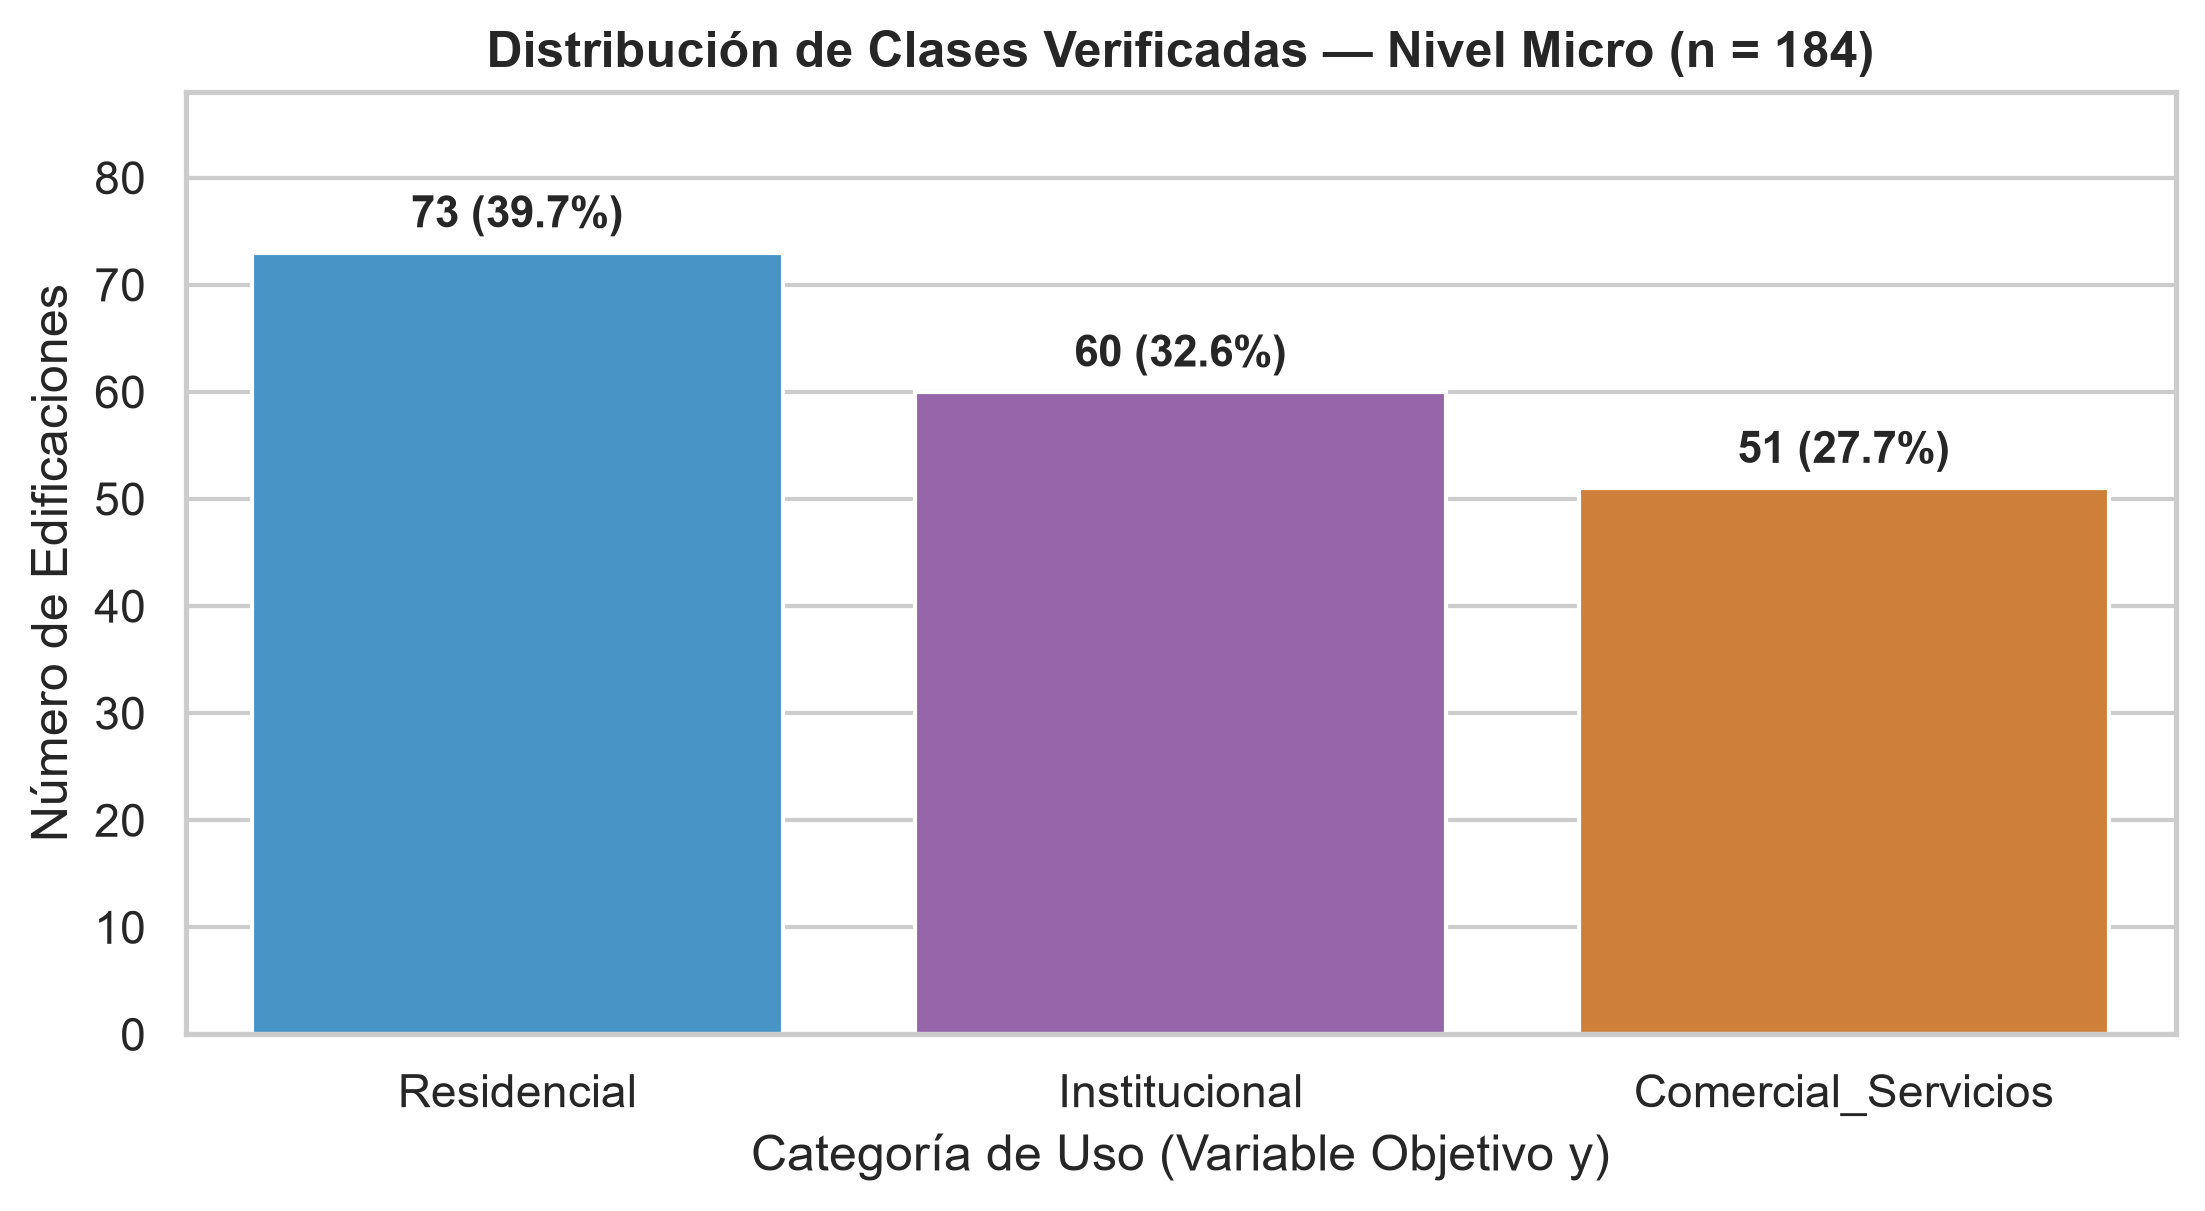
\includegraphics[width=0.72\textwidth]{figures/02_distribucion_clases_micro.png}
    \caption{Distribución de las $184$ edificaciones verificadas del Distrito de Puno en las tres categorías de la variable objetivo \texttt{clase\_uso}.}
    \label{fig:dist_micro}
\end{figure}

\subsection{Ingeniería de Variables ($X$): Morfología + Entorno Espacial con \texttt{KD-Tree}}

Cada una de las $652$ edificaciones fue proyectada a coordenadas métricas UTM Zona 19 Sur (\texttt{EPSG:32719}) para extraer \textbf{$11$ variables predictoras numéricas ($X$)} divididas en dos grupos:

\begin{itemize}[leftmargin=0.8cm, itemsep=3pt]
    \item \textbf{Variables Morfológicas ($5$ variables geométricas):} superficie construida (\texttt{area\_m2}), perímetro (\texttt{perimetro\_m}), índice de compacidad de Polsby-Popper $C = 4\pi \cdot \text{Área}/\text{Perímetro}^2 \in (0, 1]$ (\texttt{compacidad}), relación largo/ancho del rectángulo mínimo envolvente (\texttt{relacion\_aspecto}) y número de vértices del polígono (\texttt{num\_vertices}).
    \item \textbf{Variables Espaciales y de Proximidad ($6$ variables):} distancia a la Plaza de Armas (\texttt{dist\_plaza\_armas\_m}), distancia a la vía más cercana (\texttt{dist\_via\_cercana\_m}), jerarquía vial codificada de $0$ a $3$ (\texttt{jerarquia\_via}), y tres métricas de vecindad calculadas mediante \textbf{\texttt{cKDTree}}: \texttt{densidad\_edificios\_150m}, \texttt{dist\_vecino\_cercano\_m} y \texttt{pois\_entorno\_300m}.
\end{itemize}


La Tabla~\ref{tab:medianas_micro} presenta las medianas de las $11$ variables agrupadas por clase urbana verificada.

\begin{table}[H]
    \centering
    \caption{Medianas de las $11$ variables predictoras ($X$) según la categoría urbana en el Nivel Micro ($n = 184$).}
    \label{tab:medianas_micro}
    \setlength{\tabcolsep}{6pt}
    \small
    \begin{adjustbox}{max width=\textwidth}
    \begin{tabular}{lrrr}
        \toprule
        \rowcolor{verdeHeader}
        \textcolor{white}{\textbf{Variable Predictora ($X$)}} & \textcolor{white}{\textbf{Comercial\_Servicios}} & \textcolor{white}{\textbf{Institucional}} & \textcolor{white}{\textbf{Residencial}} \\
        \midrule
        \texttt{area\_m2} ($\text{m}^2$) & 399.75 & 347.19 & 110.88 \\
        \rowcolor{verdeSuave!50}
        \texttt{perimetro\_m} (m) & 87.64 & 84.90 & 44.88 \\
        \texttt{compacidad} (Polsby-Popper) & 0.63 & 0.67 & 0.67 \\
        \rowcolor{verdeSuave!50}
        \texttt{relacion\_aspecto} (largo/ancho) & 1.72 & 1.79 & 1.95 \\
        \texttt{num\_vertices} & 6.00 & 4.00 & 4.00 \\
        \rowcolor{verdeSuave!50}
        \texttt{dist\_plaza\_armas\_m} (m) & 433.20 & 998.97 & 785.81 \\
        \texttt{dist\_via\_cercana\_m} (m) & 3.09 & 5.21 & 4.79 \\
        \rowcolor{verdeSuave!50}
        \texttt{jerarquia\_via} (0--3) & 1.00 & 1.00 & 1.00 \\
        \texttt{densidad\_edificios\_150m} (\texttt{cKDTree}) & 11.00 & 10.00 & 24.00 \\
        \rowcolor{verdeSuave!50}
        \texttt{dist\_vecino\_cercano\_m} (\texttt{cKDTree}, m) & 25.20 & 33.26 & 10.92 \\
        \texttt{pois\_entorno\_300m} (\texttt{cKDTree}) & 98.00 & 13.00 & 24.00 \\
        \bottomrule
    \end{tabular}
    \end{adjustbox}
\end{table}


\subsection{¿Cómo Validamos Nuestros Modelos?}

Para evitar confusiones metodológicas frecuentes, es fundamental distinguir dos fases completamente separadas en el manejo de las $652$ edificaciones (Figura~\ref{fig:flujo_validacion_micro}):

\begin{enumerate}[leftmargin=0.85cm, itemsep=3pt]
    \item \textbf{Fase de Evaluación Supervisada (únicamente sobre las $184$ edificaciones verificadas):}
    \begin{itemize}[leftmargin=0.6cm, itemsep=1pt]
        \item \textbf{80\% Entrenamiento (\textit{Train} = $147$ edificaciones):} datos con los que cada modelo aprende las reglas que vinculan $X \rightarrow y$.
        \item \textbf{20\% Prueba (\textit{Test} = $37$ edificaciones):} \textbf{no} se usa para imputar los edificios faltantes; corresponde a edificaciones cuya etiqueta real sí conocemos en OSM, pero que ocultamos temporalmente a los algoritmos para simular un \textbf{``examen final''} y construir la matriz de confusión de manera imparcial. La partición es \textbf{estratificada} para conservar exactamente las mismas proporciones de las 3 clases en Train y Test.
        \item \textbf{Validación Cruzada Estratificada de 5 Pliegues (\texttt{5-Fold Stratified CV}):} divide los datos etiquetados en cinco bloques iguales; en cinco rondas rotativas, cuatro bloques ($80\%$) entrenan y el bloque restante ($20\%$) evalúa. El promedio de las cinco rondas (\texttt{CV-5 F1-Macro}) garantiza que el modelo ganador sea verdaderamente el que mejor generaliza y no el resultado de una partición afortunada.
    \end{itemize}
    \item \textbf{Fase de Imputación (sobre las $468$ edificaciones sin etiqueta):} Estas $468$ observaciones nunca ingresan ni al entrenamiento ni al examen porque carecen de etiqueta real en OSM. Únicamente tras elegir al ganador en la Fase~1, dicho modelo se reentrena con el $100\%$ de las $184$ verificadas y predice el uso de las $468$ edificaciones faltantes.
\end{enumerate}

\begin{figure}[H]
    \centering
    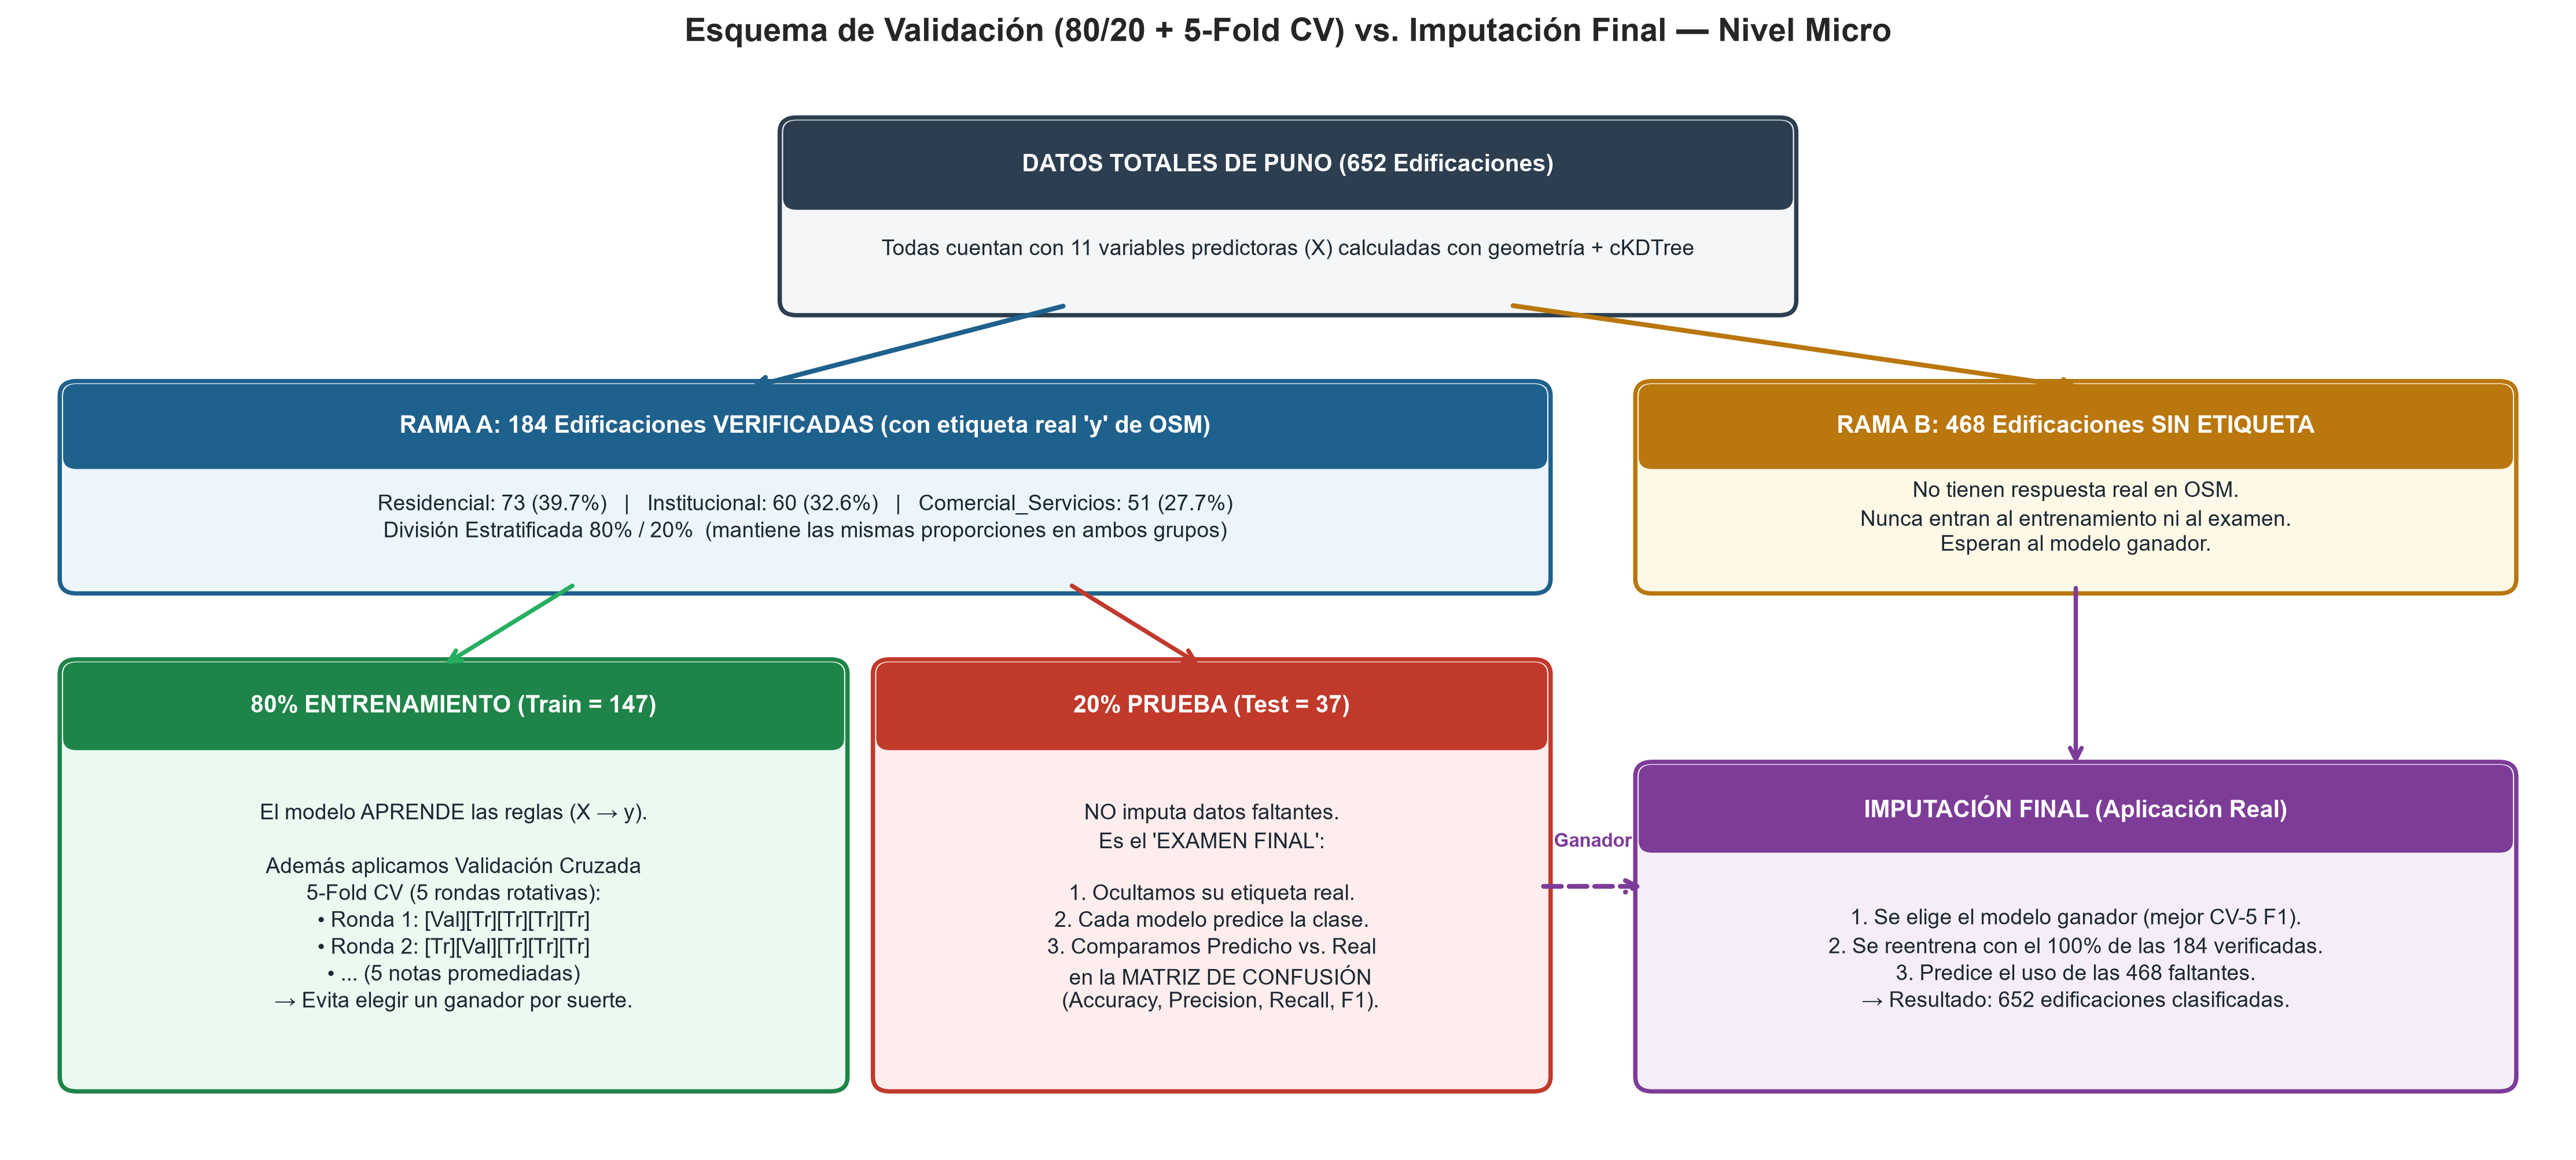
\includegraphics[width=0.98\textwidth]{figures/02_flujo_validacion_micro.png}
    \caption{Esquema metodológico de validación (partición estratificada 80/20 + 5-Fold CV sobre las $184$ verificadas) separado de la imputación final de las $468$ edificaciones sin etiqueta.}
    \label{fig:flujo_validacion_micro}
\end{figure}


Antes de entrenar la comparativa final, se ejecutó un \textbf{experimento de poda} variando la profundidad máxima (\texttt{max\_depth} de $2$ a $10$) con validación cruzada 5-Fold sobre el conjunto de entrenamiento (Figura~\ref{fig:poda_micro}).

\begin{figure}[H]
    \centering
    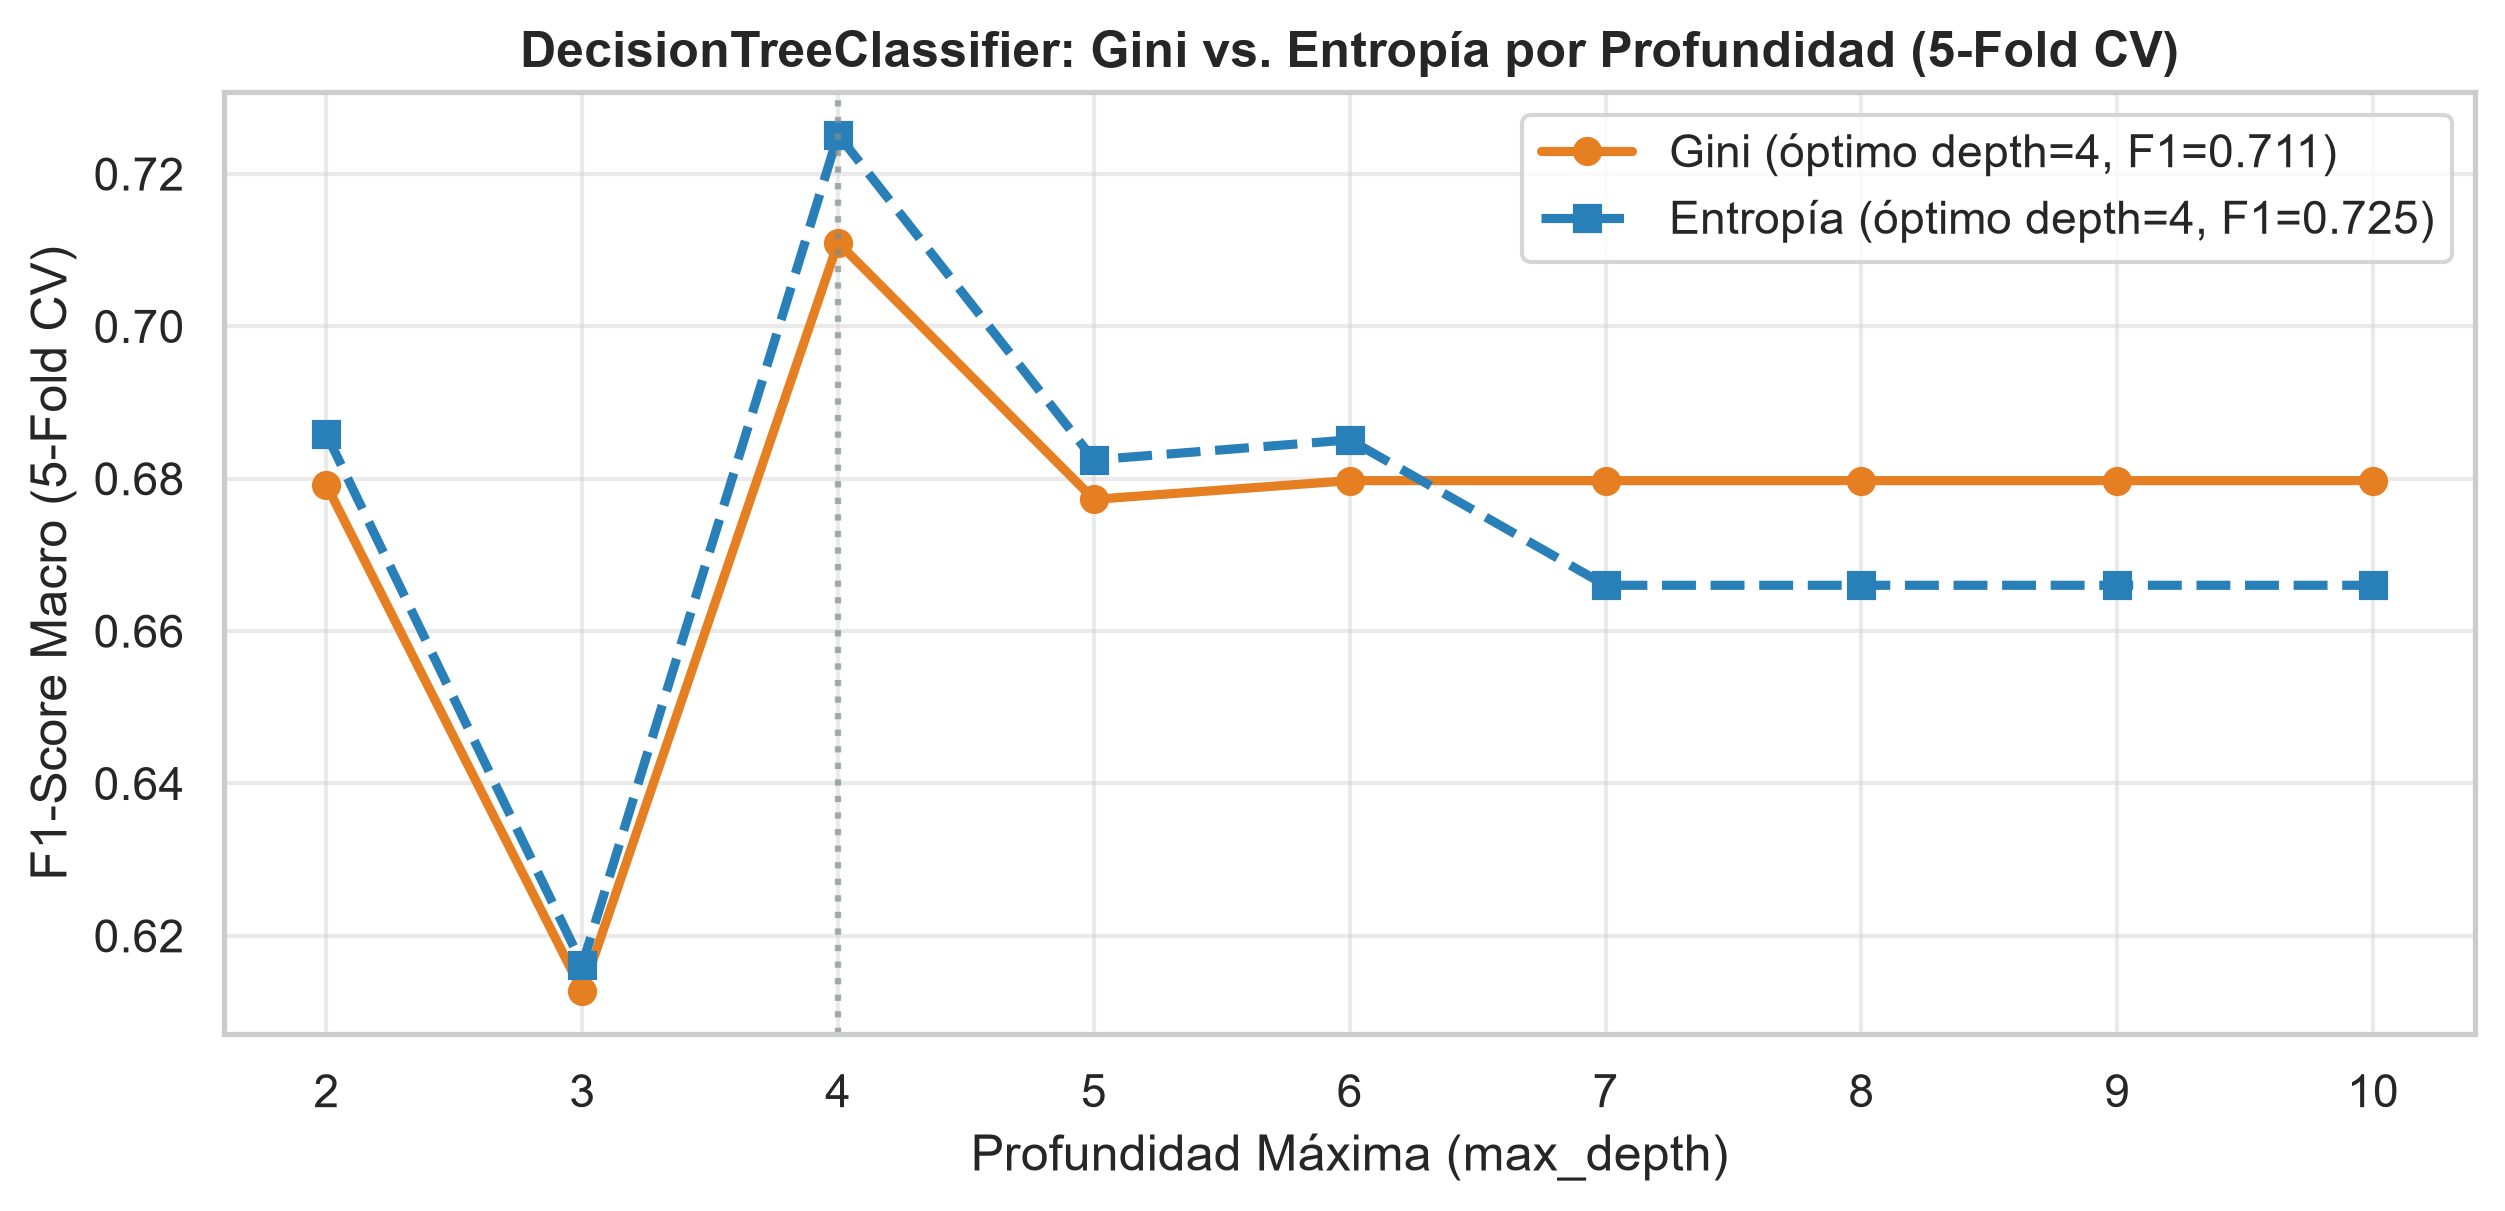
\includegraphics[width=0.82\textwidth]{figures/02_poda_gini_vs_entropia_micro.png}
    \caption{Experimento de poda (\texttt{max\_depth} de $2$ a $10$) comparando los criterios de Gini y Entropía mediante F1-Score Macro en validación cruzada 5-Fold (Nivel Micro).}
    \label{fig:poda_micro}
\end{figure}

\subsection{Entrenamiento y Tabla Comparativa de los 4 Modelos (5 Configuraciones)}

Se entrenaron las cinco configuraciones sobre la misma partición estratificada ($147$ entrenamiento / $37$ prueba) y se evaluaron en 5-Fold CV midiendo además el tiempo de cómputo (Tabla~\ref{tab:resultados_micro_nb02}).

\begin{table}[H]
    \centering
    \caption{Tabla comparativa de métricas y tiempo de entrenamiento de los 4 modelos (5 configuraciones) — Nivel Micro.}
    \label{tab:resultados_micro_nb02}
    \setlength{\tabcolsep}{4pt}
    \footnotesize
    \begin{adjustbox}{max width=\textwidth}
    \begin{tabular}{lccccccc}
        \toprule
        \rowcolor{verdeHeader}
        \textcolor{white}{\textbf{Modelo}} & \textcolor{white}{\textbf{Test Acc}} & \textcolor{white}{\textbf{Test Prec (M)}} & \textcolor{white}{\textbf{Test Rec (M)}} & \textcolor{white}{\textbf{Test F1 (M)}} & \textcolor{white}{\textbf{CV-5 Acc}} & \textcolor{white}{\textbf{CV-5 F1 (M)}} & \textcolor{white}{\textbf{Tiempo (ms)}} \\
        \midrule
        \textbf{LightGBM} \textit{(Ganador CV)} & 0.8108 & 0.7879 & 0.7889 & 0.7874 & \textbf{0.7667} & \textbf{0.7496} & 63.35 \\
        \rowcolor{verdeSuave!50}
        \textbf{Random Forest} \textit{(Ganador Test)} & \textbf{0.8378} & \textbf{0.8681} & \textbf{0.8333} & \textbf{0.8115} & 0.7664 & 0.7465 & 408.88 \\
        XGBoost & 0.7838 & 0.7676 & 0.7667 & 0.7545 & 0.7395 & 0.7160 & 254.47 \\
        \rowcolor{verdeSuave!50}
        DecisionTree (Entropía) & 0.6757 & 0.6347 & 0.6500 & 0.6204 & 0.7009 & 0.6744 & 1.87 \\
        DecisionTree (Gini) & 0.8108 & 0.8125 & 0.8000 & 0.7831 & 0.6793 & 0.6517 & \textbf{1.76} \\
        \bottomrule
    \end{tabular}
    \end{adjustbox}
\end{table}

\subsection{Visualización Completa de los Árboles en los 4 Modelos}

Para dominar el funcionamiento interno de los cuatro algoritmos, se visualizaron sus árboles reales \textbf{de forma completa hasta todas sus hojas terminales (sin recortes)}.

\subsubsection{Modelo 1A — \texttt{DecisionTreeClassifier} (Criterio Gini Completo)}

\begin{figure}[H]
    \centering
    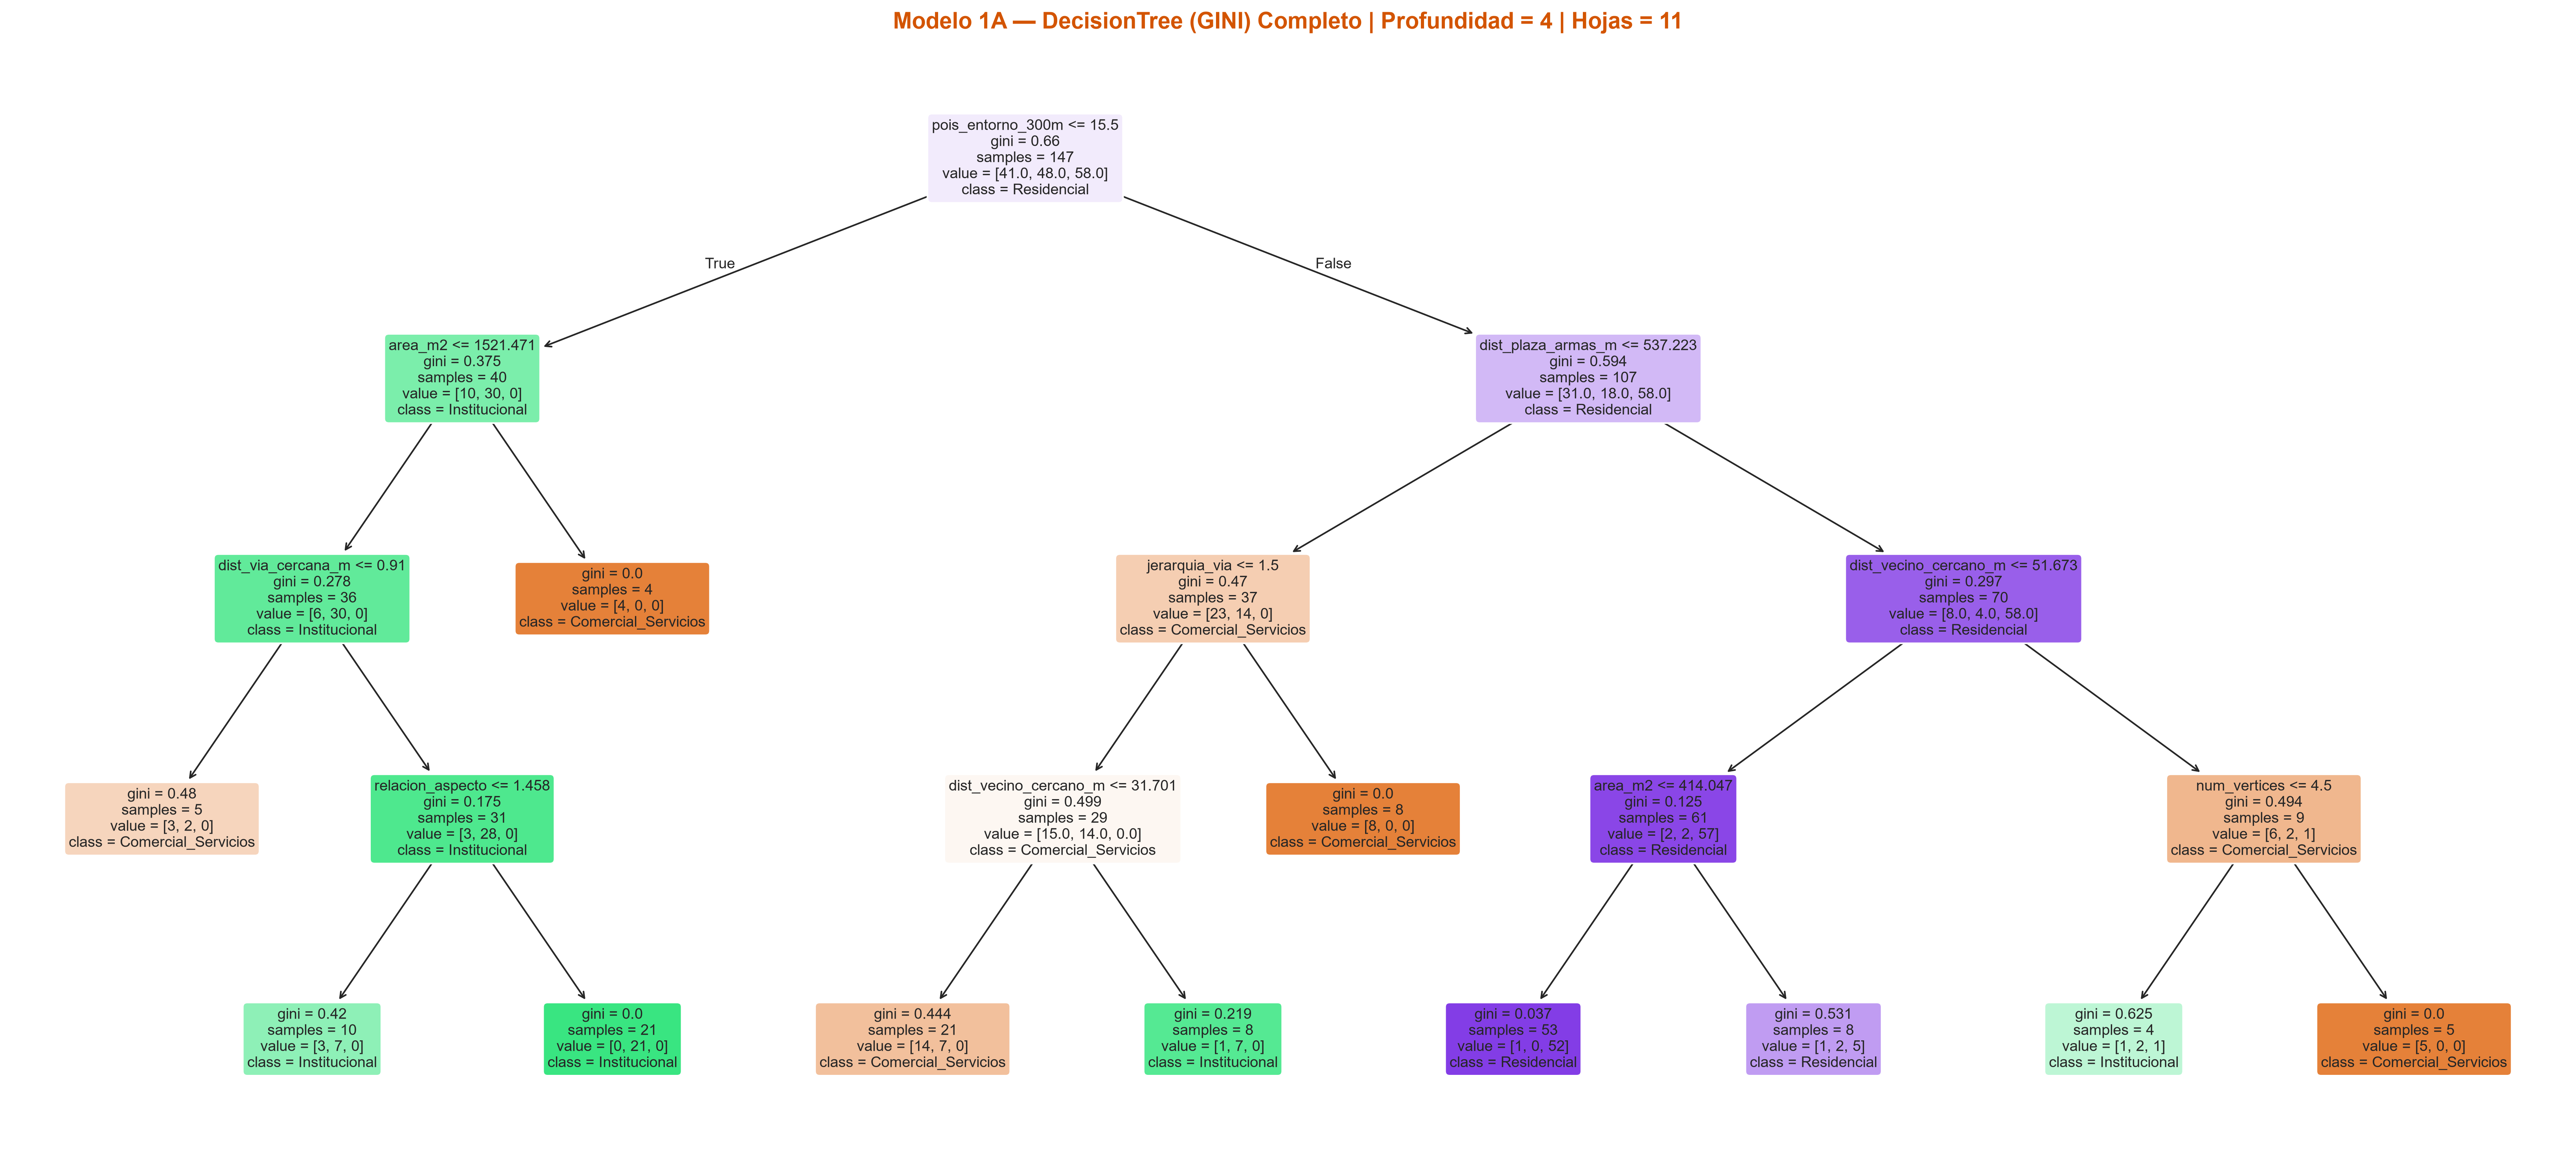
\includegraphics[width=0.99\textwidth]{figures/02_arbol_gini_completo.png}
    \caption{Árbol completo de \texttt{DecisionTreeClassifier} con criterio \textbf{Gini} en el Nivel Micro (profundidad $= 4$, $11$ hojas terminales).}
    \label{fig:nb02_gini}
\end{figure}


\subsubsection{Modelo 1B — \texttt{DecisionTreeClassifier} (Criterio Entropía Completo)}

\begin{figure}[H]
    \centering
    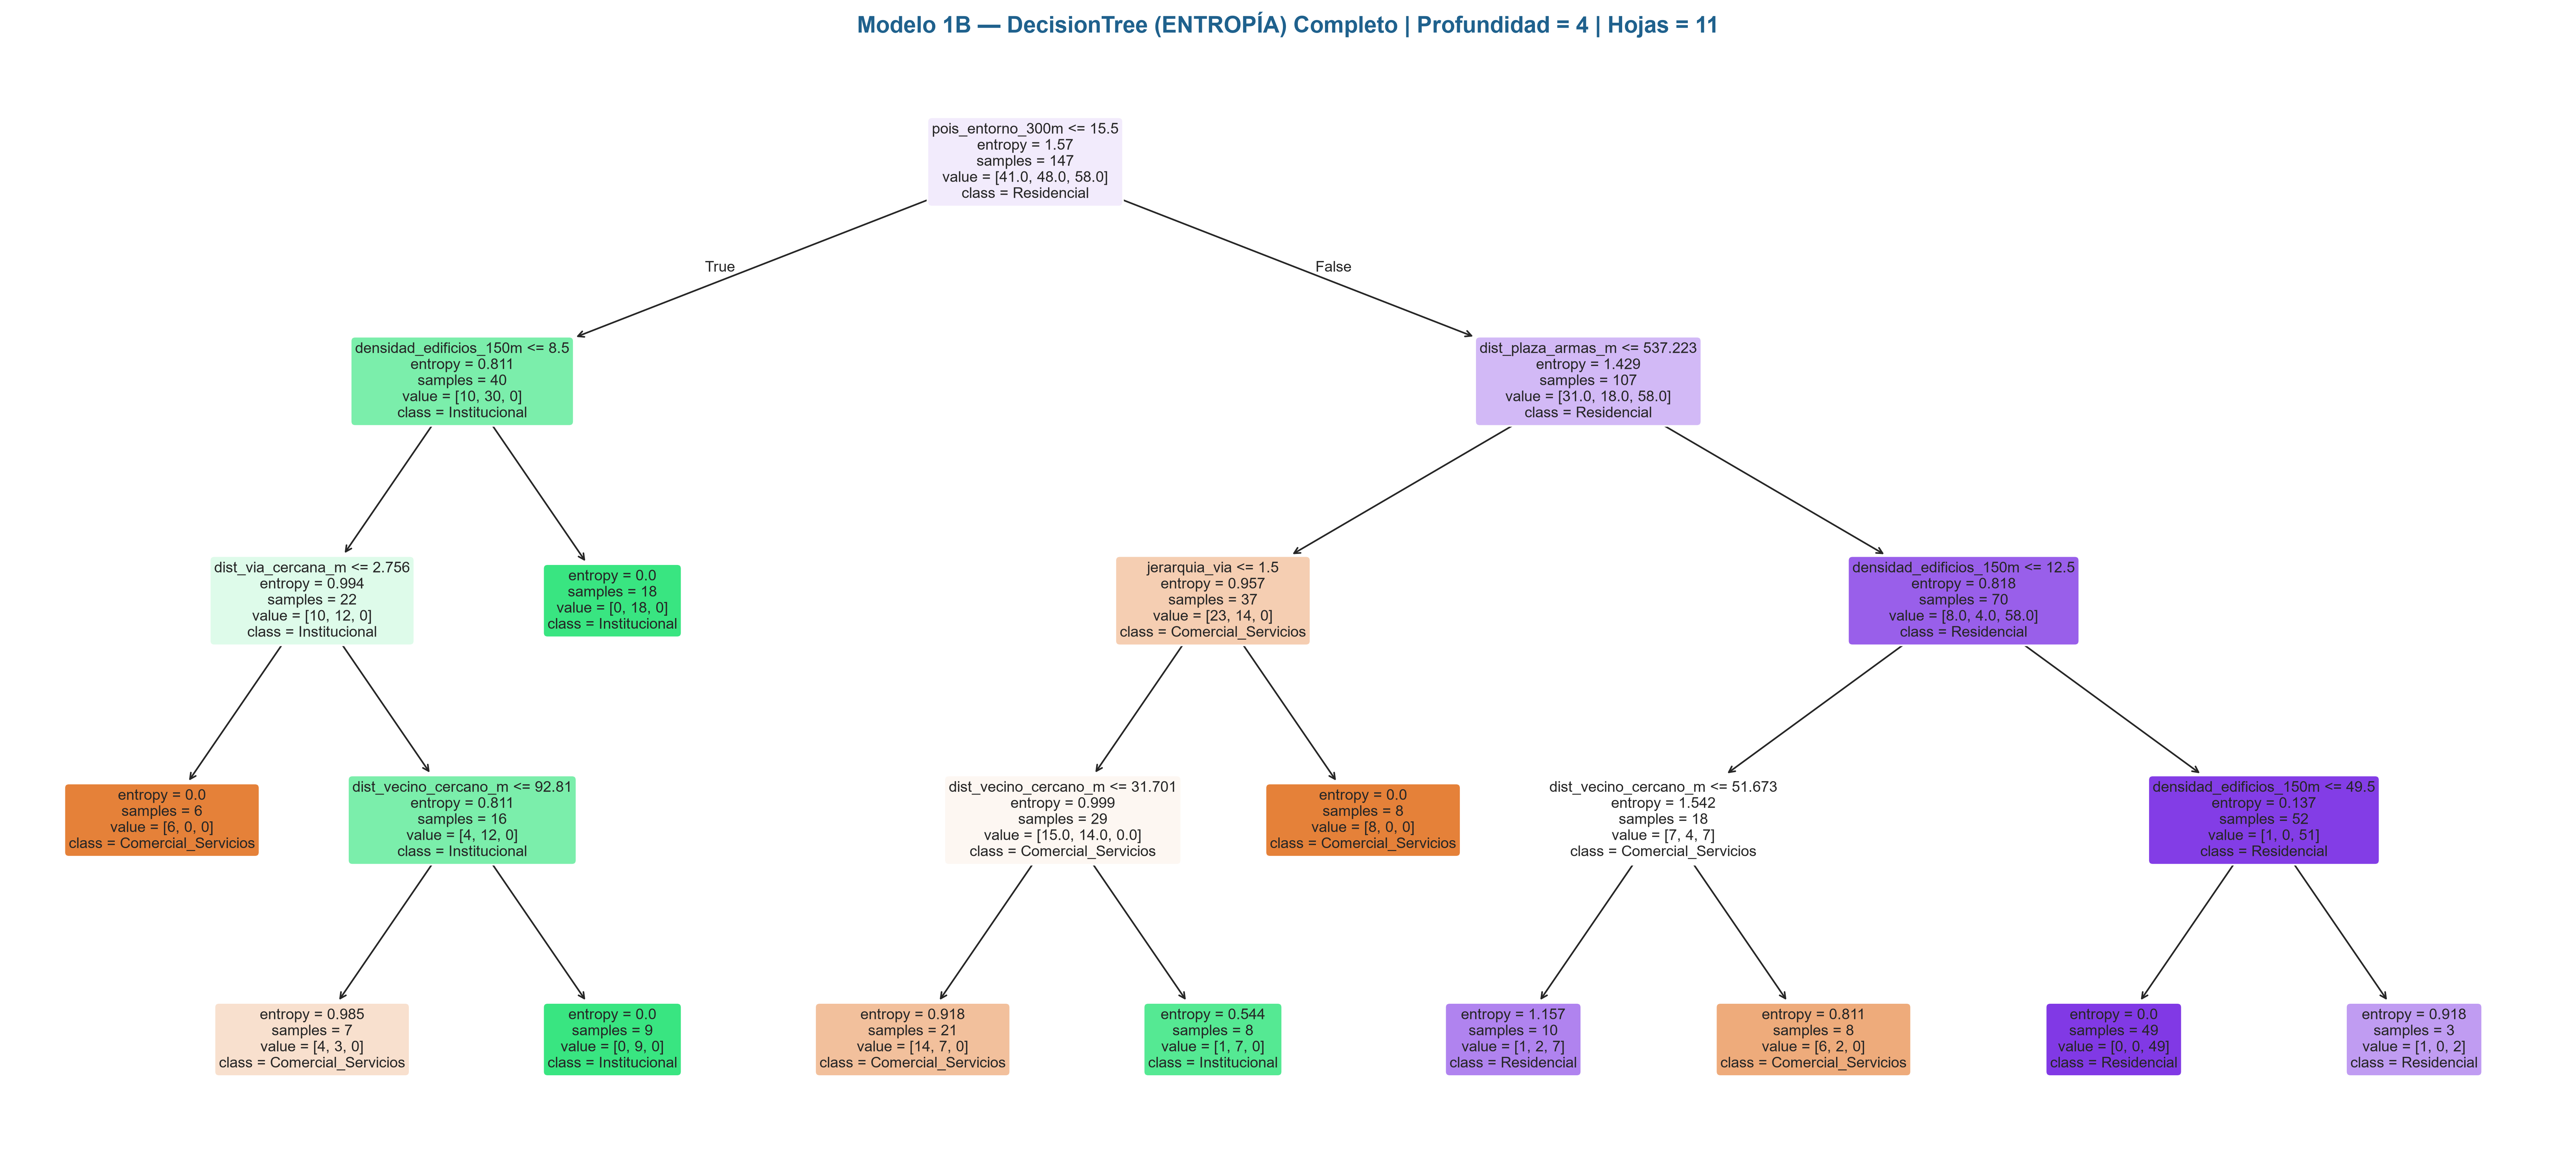
\includegraphics[width=0.99\textwidth]{figures/02_arbol_entropia_completo.png}
    \caption{Árbol completo de \texttt{DecisionTreeClassifier} con criterio \textbf{Entropía} en el Nivel Micro (profundidad $= 4$, $11$ hojas terminales).}
    \label{fig:nb02_entropia}
\end{figure}

\subsubsection{Modelo 2 — \texttt{RandomForestClassifier} (\textit{Bagging}): Árbol \#1 y Árbol \#200 Completos}

Random Forest entrena $200$ árboles profundos e independientes en paralelo. Las Figuras~\ref{fig:nb02_rf1} y~\ref{fig:nb02_rf200} muestran completos el \textbf{primer árbol (\#1)} y el \textbf{último árbol (\#200)} del bosque.

\begin{figure}[H]
    \centering
    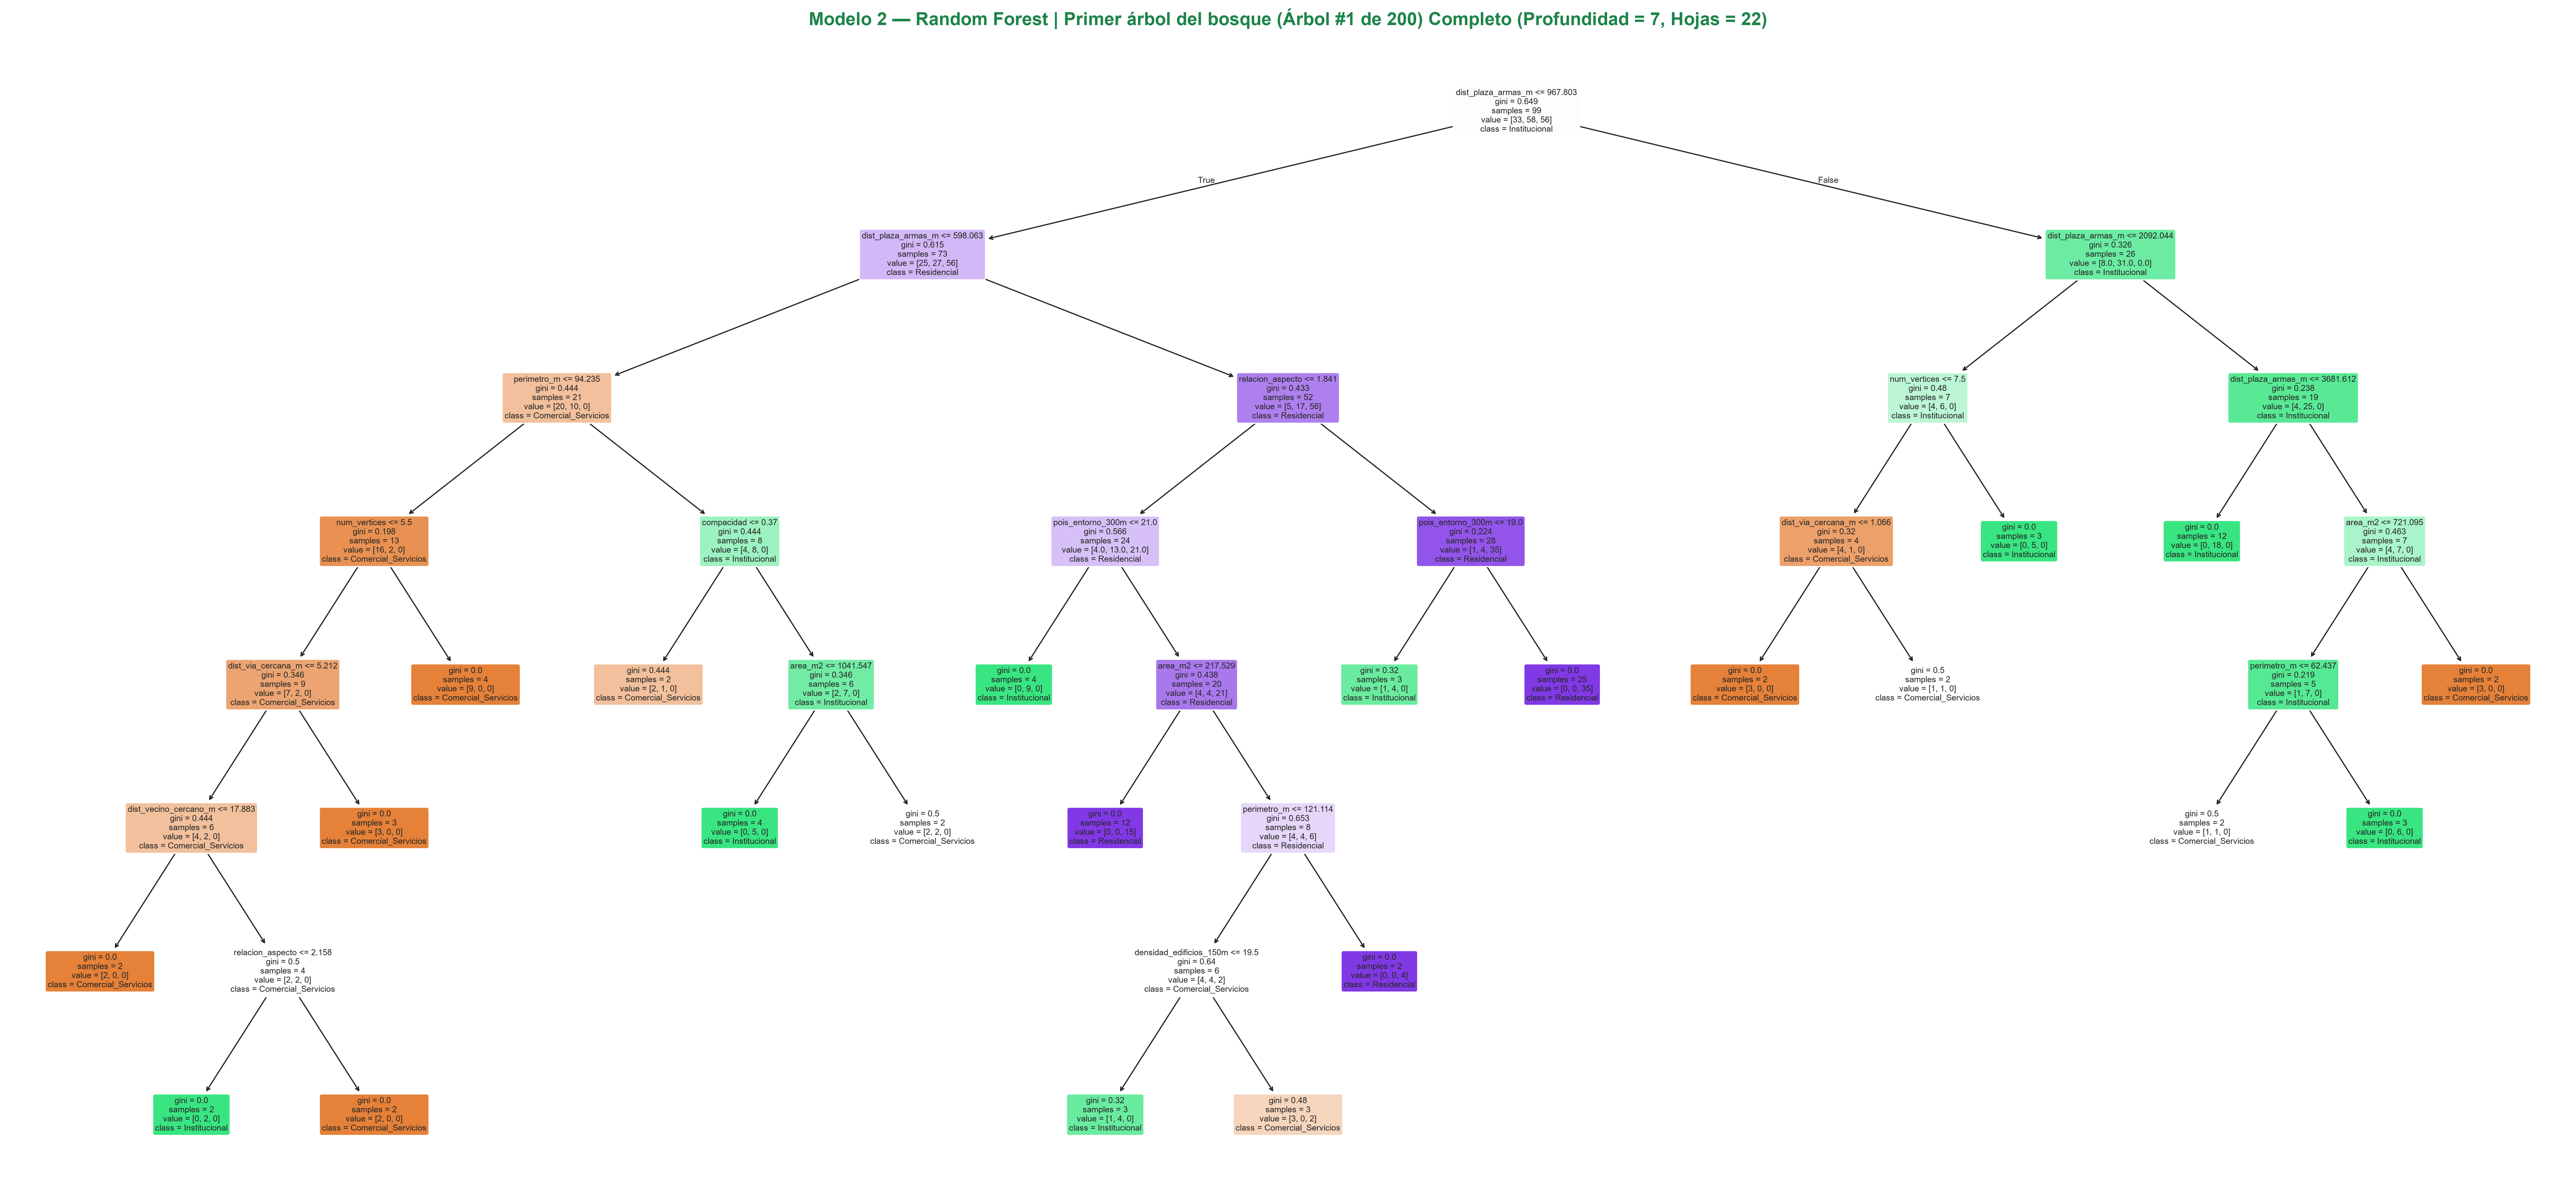
\includegraphics[width=0.99\textwidth]{figures/02_arbol_rf_001_completo.png}
    \caption{Primer árbol completo del bosque \textbf{Random Forest} (Árbol \#1 de $200$, profundidad $= 7$, $22$ hojas terminales).}
    \label{fig:nb02_rf1}
\end{figure}

\begin{figure}[H]
    \centering
    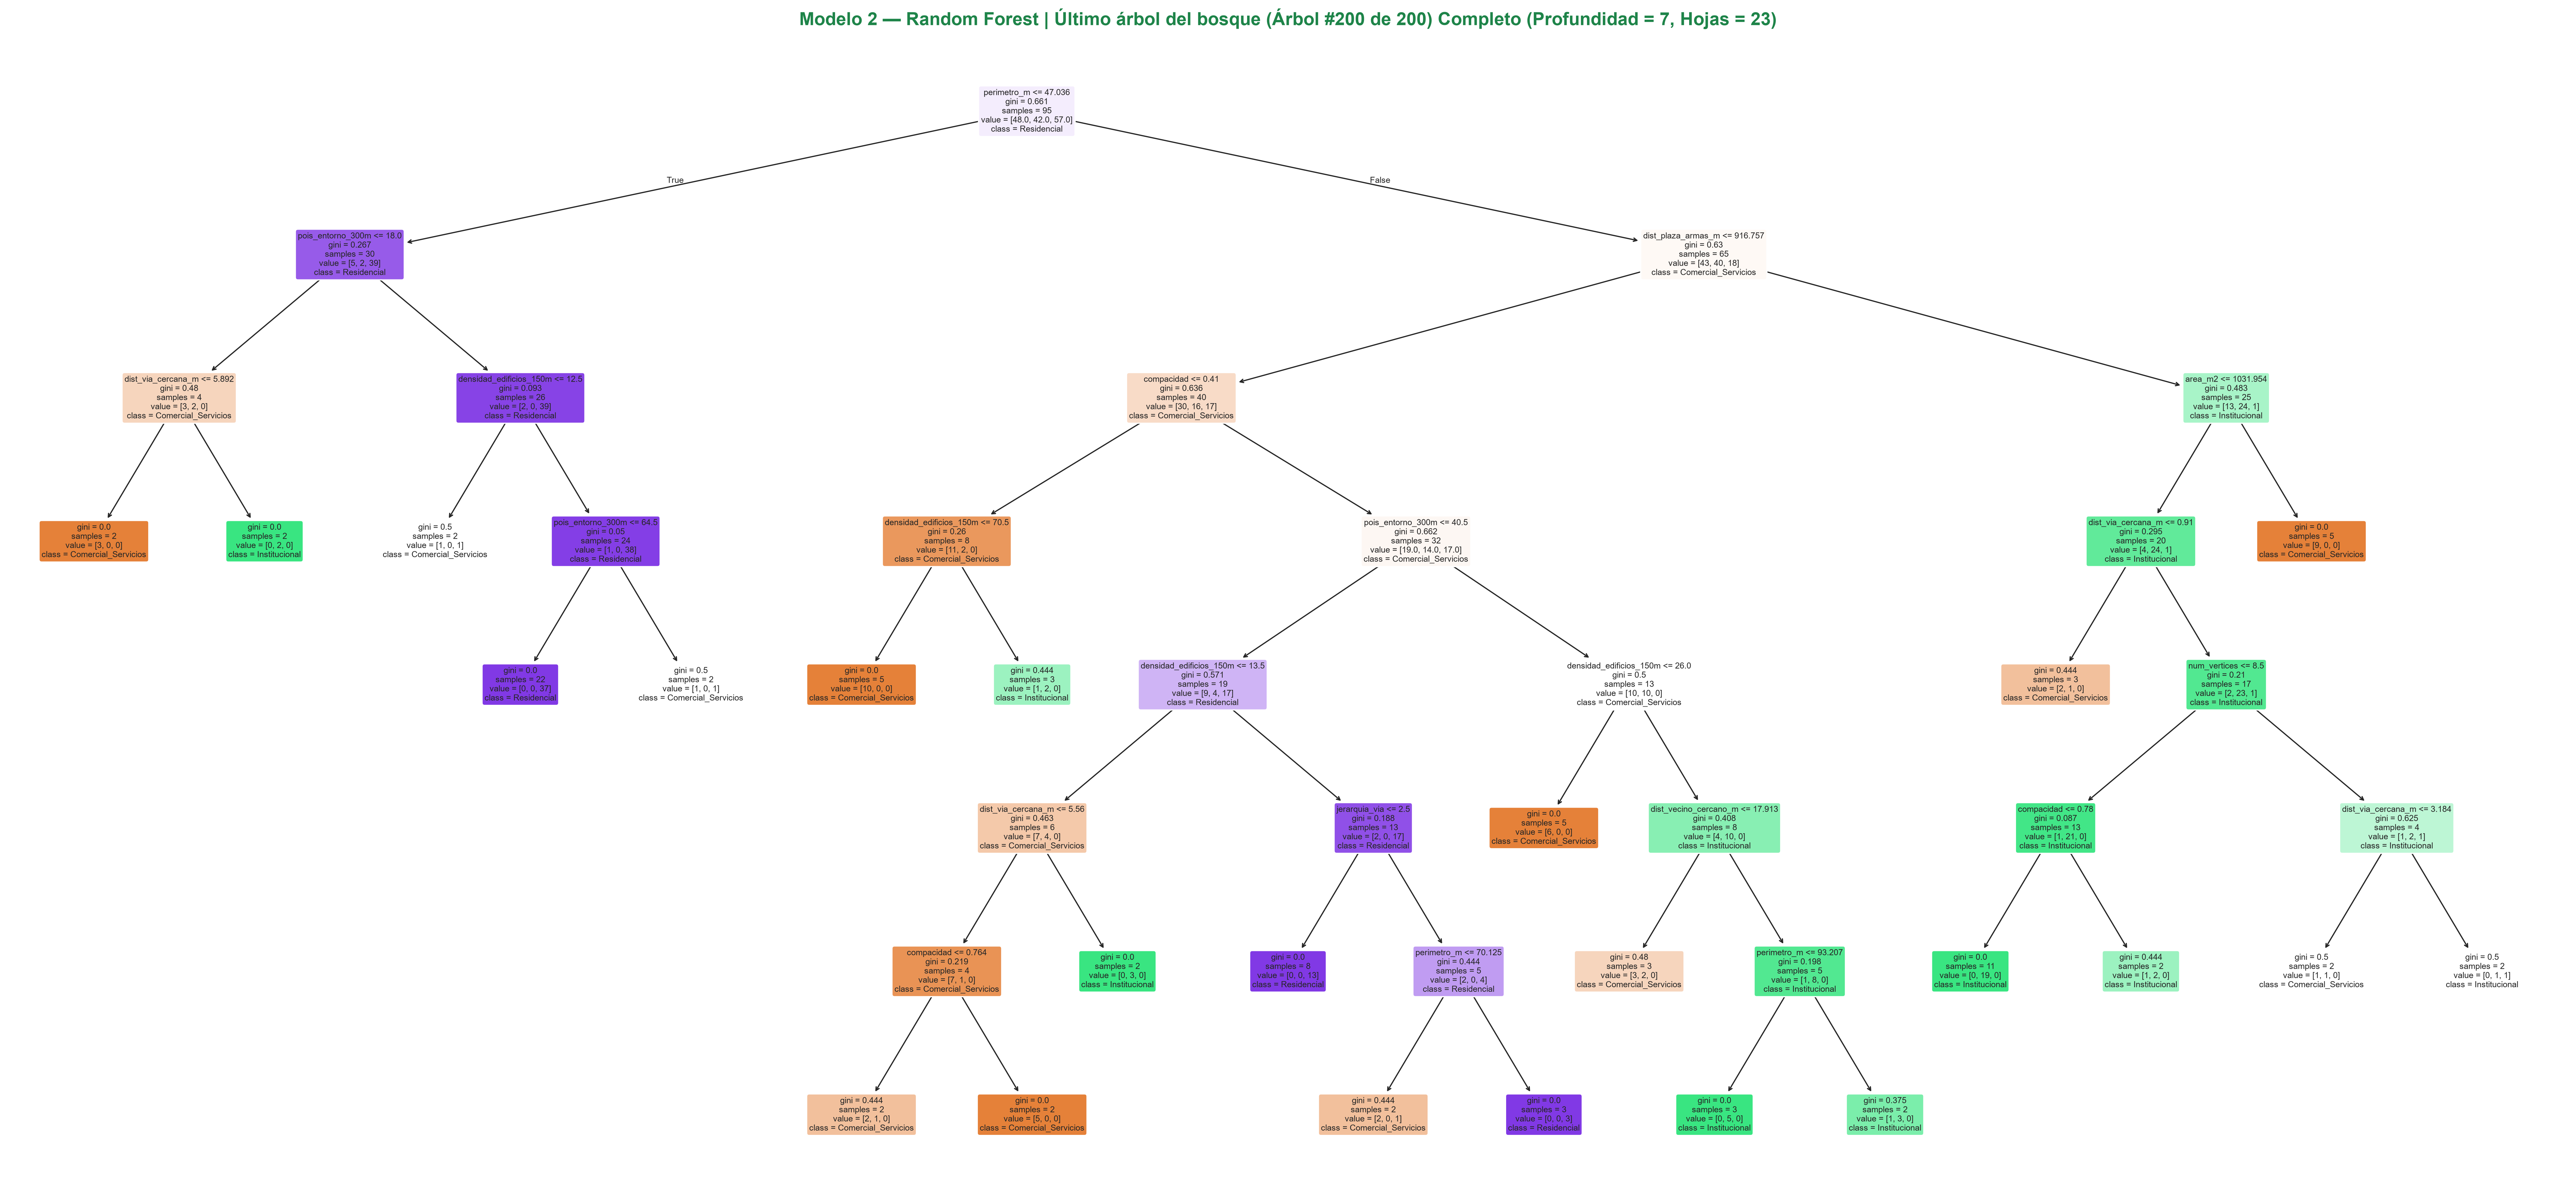
\includegraphics[width=0.99\textwidth]{figures/02_arbol_rf_200_completo.png}
    \caption{Último árbol completo del bosque \textbf{Random Forest} (Árbol \#200 de $200$, profundidad $= 7$, $23$ hojas terminales).}
    \label{fig:nb02_rf200}
\end{figure}

\subsubsection{Modelos 3 y 4 — \texttt{XGBoost} y \texttt{LightGBM} Completos (Inicio y Ronda Final \#150)}

A diferencia de Random Forest, en \textit{Boosting} los árboles sí se construyen de manera \textbf{secuencial}: cada nueva ronda corrige el error residual dejado por las rondas anteriores. Por ello, sus hojas no contienen nombres de clases sino \textbf{pesos numéricos $w^*$} (en verde los ajustes positivos que incrementan la probabilidad de la clase y en rojo los ajustes negativos que la reducen). Las Figuras~\ref{fig:nb02_xgb1} y~\ref{fig:nb02_xgb150} muestran la Ronda~1 y la Ronda Final~\#150 de \textbf{XGBoost}, mientras que las Figuras~\ref{fig:nb02_lgbm2} y~\ref{fig:nb02_lgbm150} muestran el inicio y la Ronda Final~\#150 de \textbf{LightGBM}.

\begin{figure}[H]
    \centering
    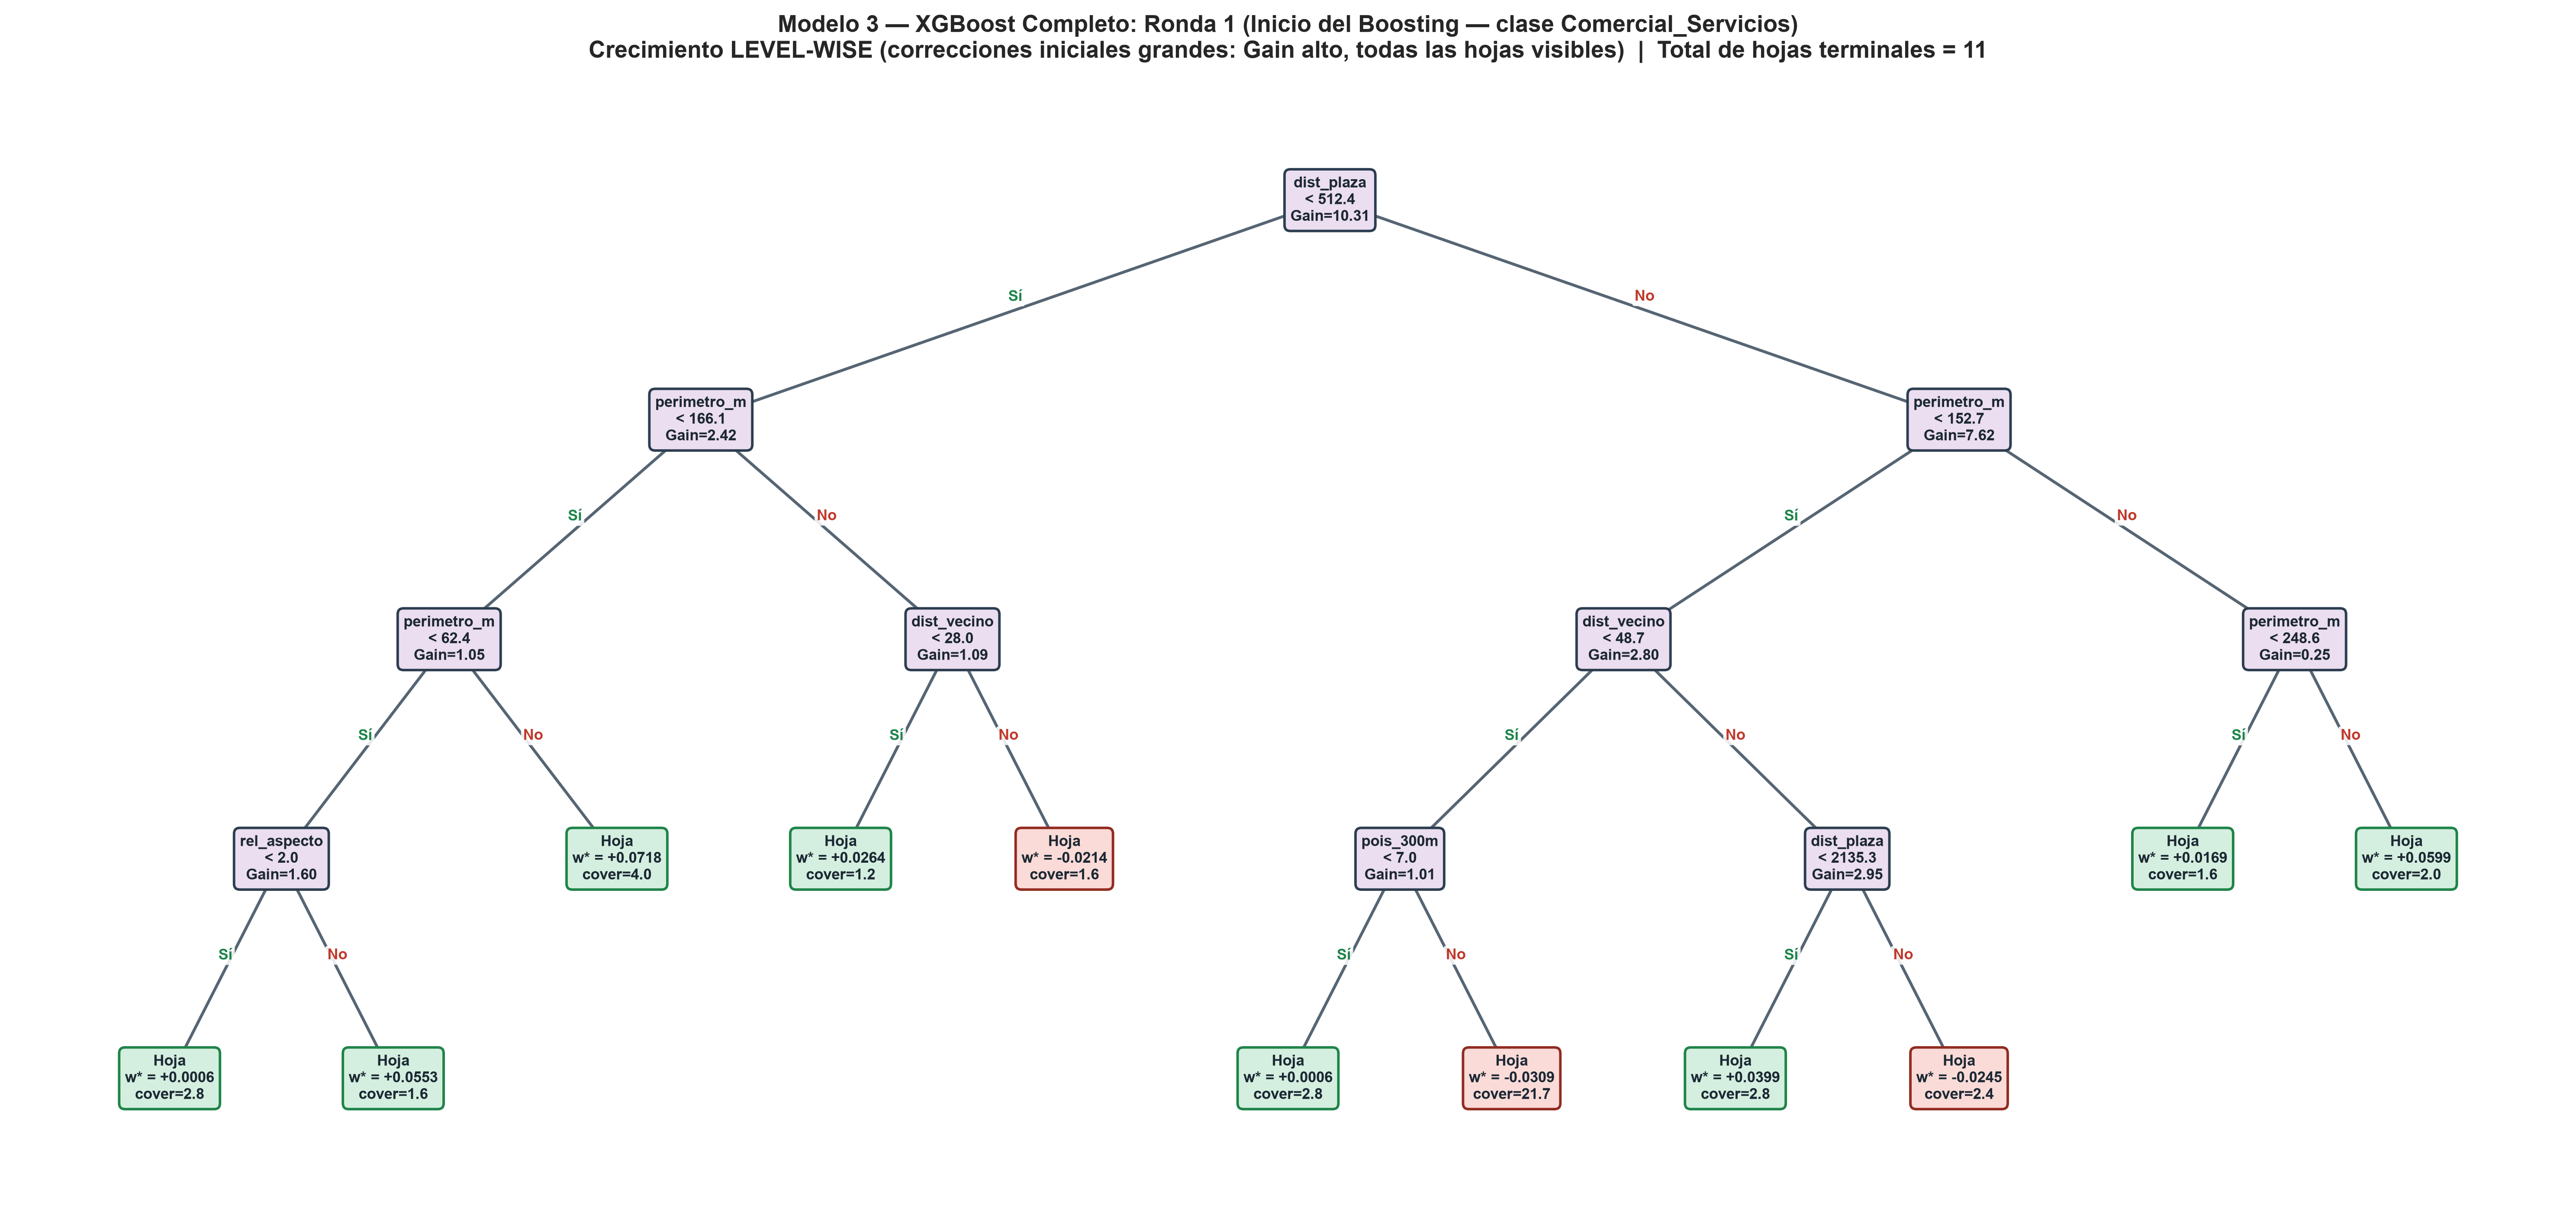
\includegraphics[width=0.98\textwidth]{figures/02_arbol_xgboost_ronda1_completo.png}
    \caption{Árbol completo de \textbf{XGBoost} en la Ronda~1 (clase \texttt{Comercial\_Servicios}, $11$ hojas terminales): crecimiento equilibrado por niveles (\textit{level-wise}) con ganancias iniciales altas.}
    \label{fig:nb02_xgb1}
\end{figure}

\begin{figure}[H]
    \centering
    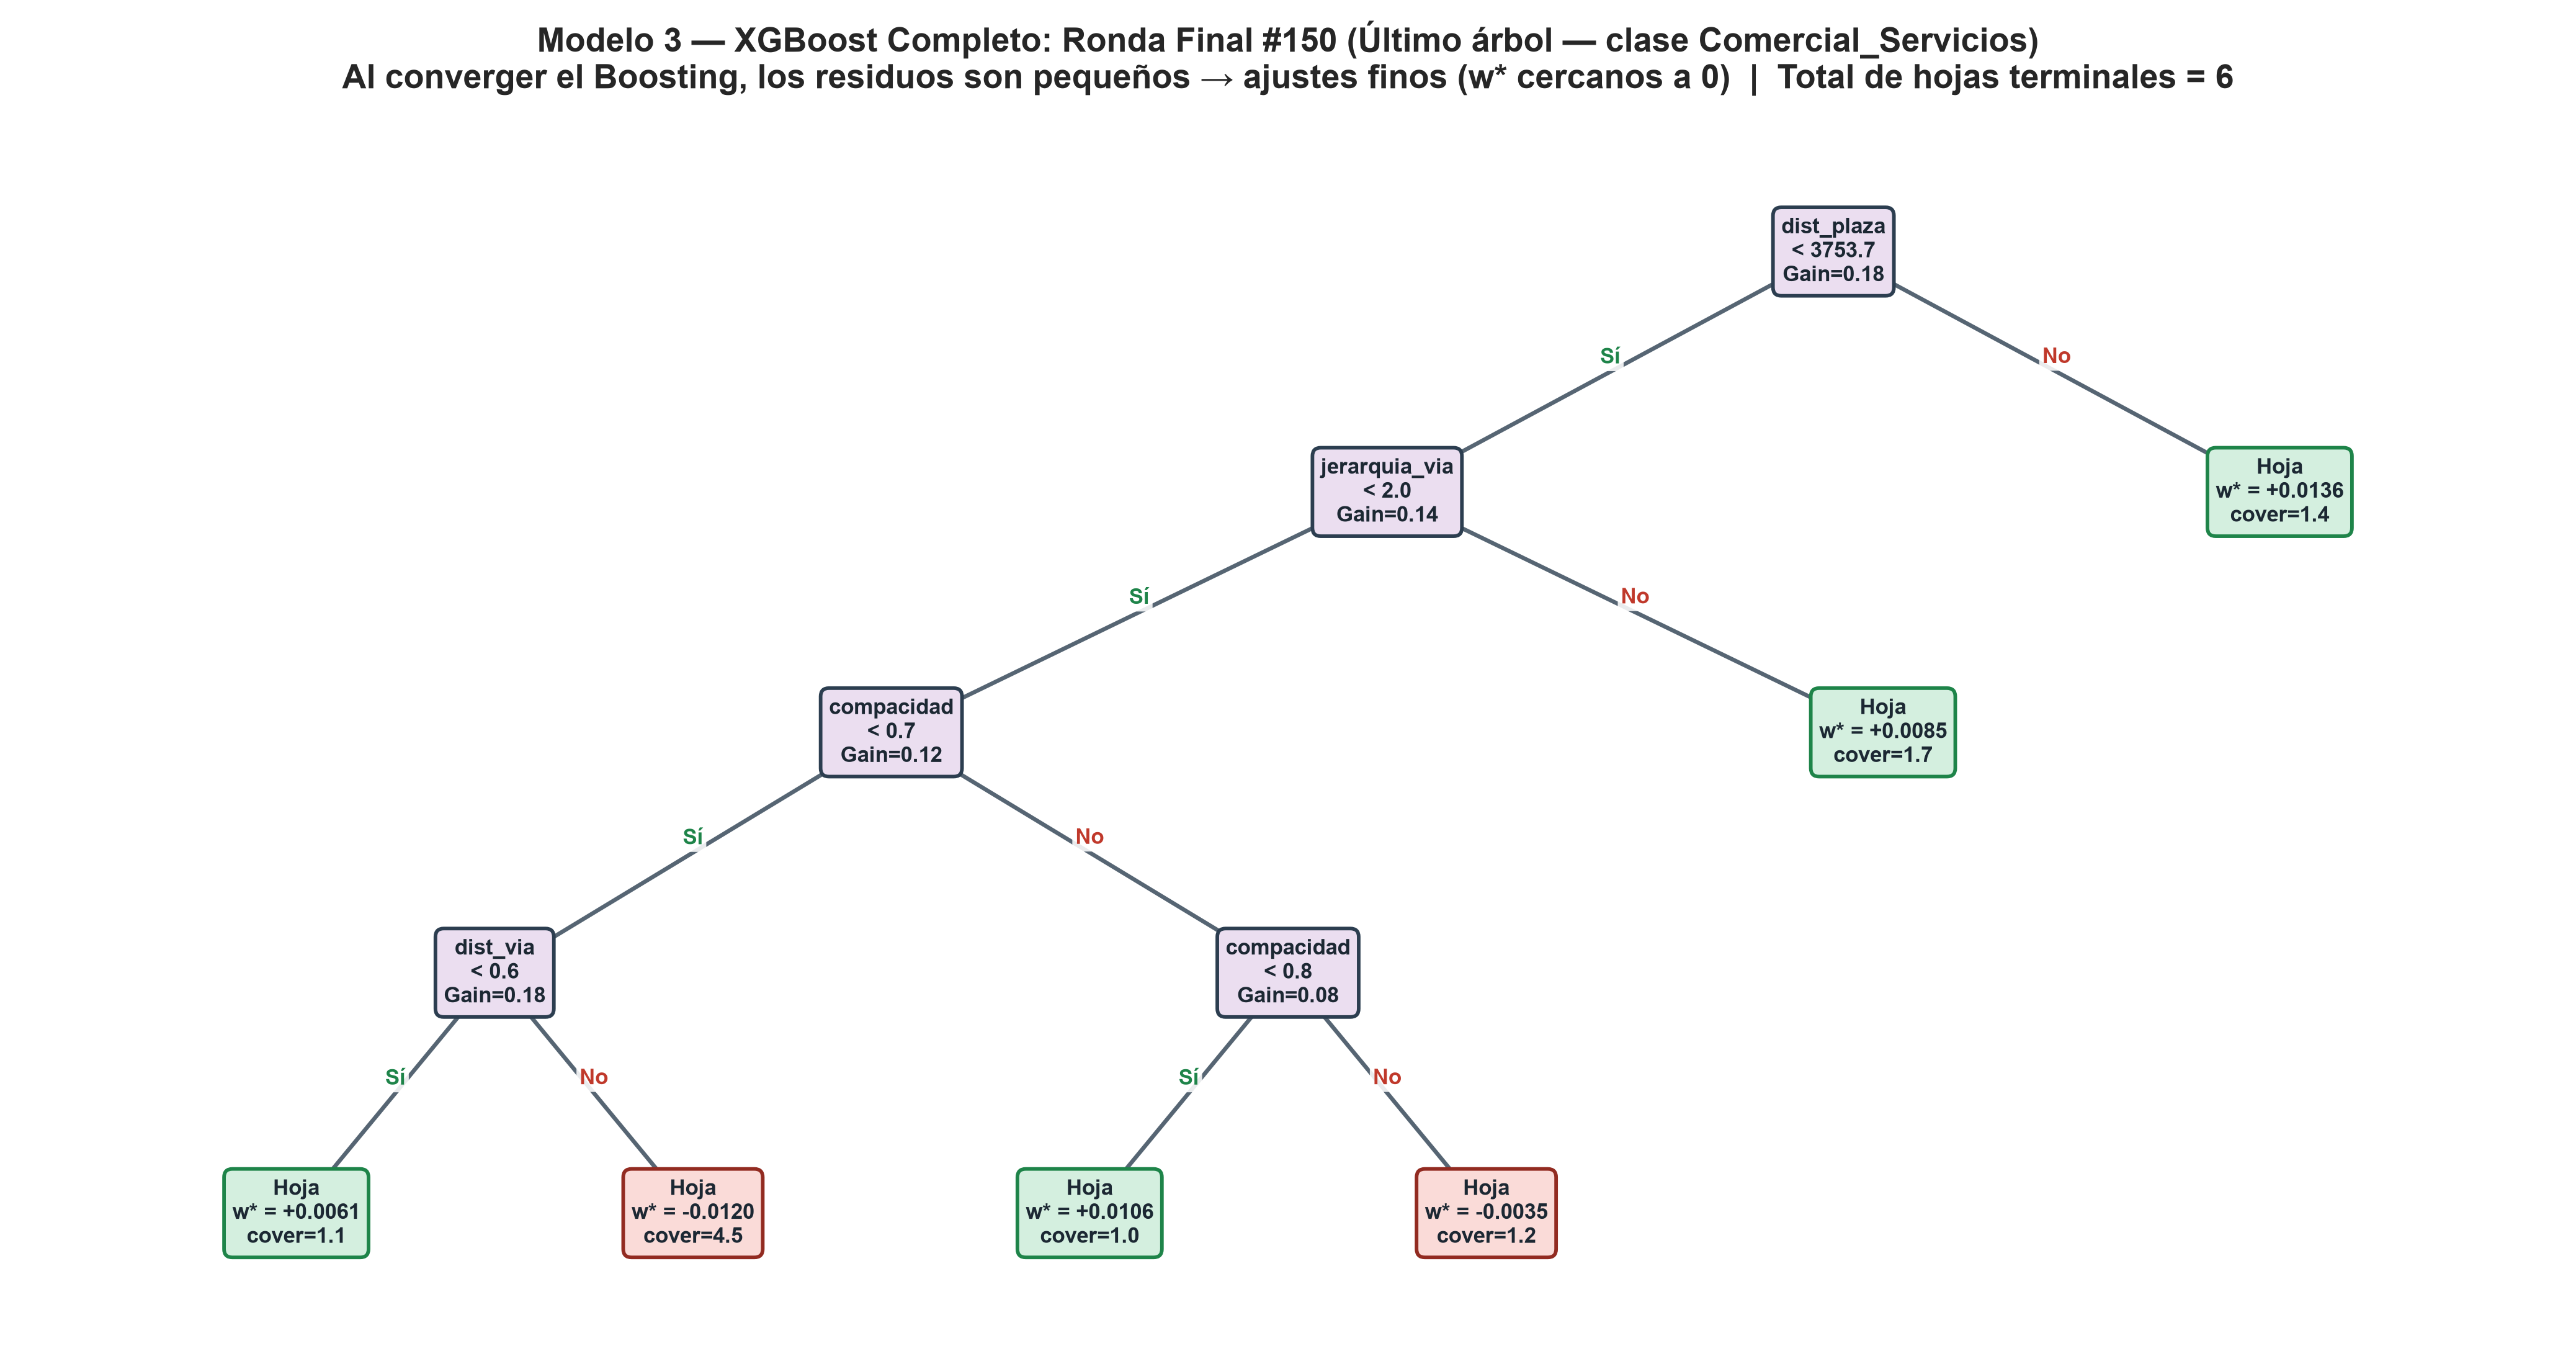
\includegraphics[width=0.84\textwidth]{figures/02_arbol_xgboost_ronda150_completo.png}
    \caption{Árbol completo de \textbf{XGBoost} en la Ronda Final~\#150 ($6$ hojas terminales): evidencia la convergencia del Boosting mediante ganancias y pesos $w^*$ cercanos a cero.}
    \label{fig:nb02_xgb150}
\end{figure}


\begin{figure}[H]
    \centering
    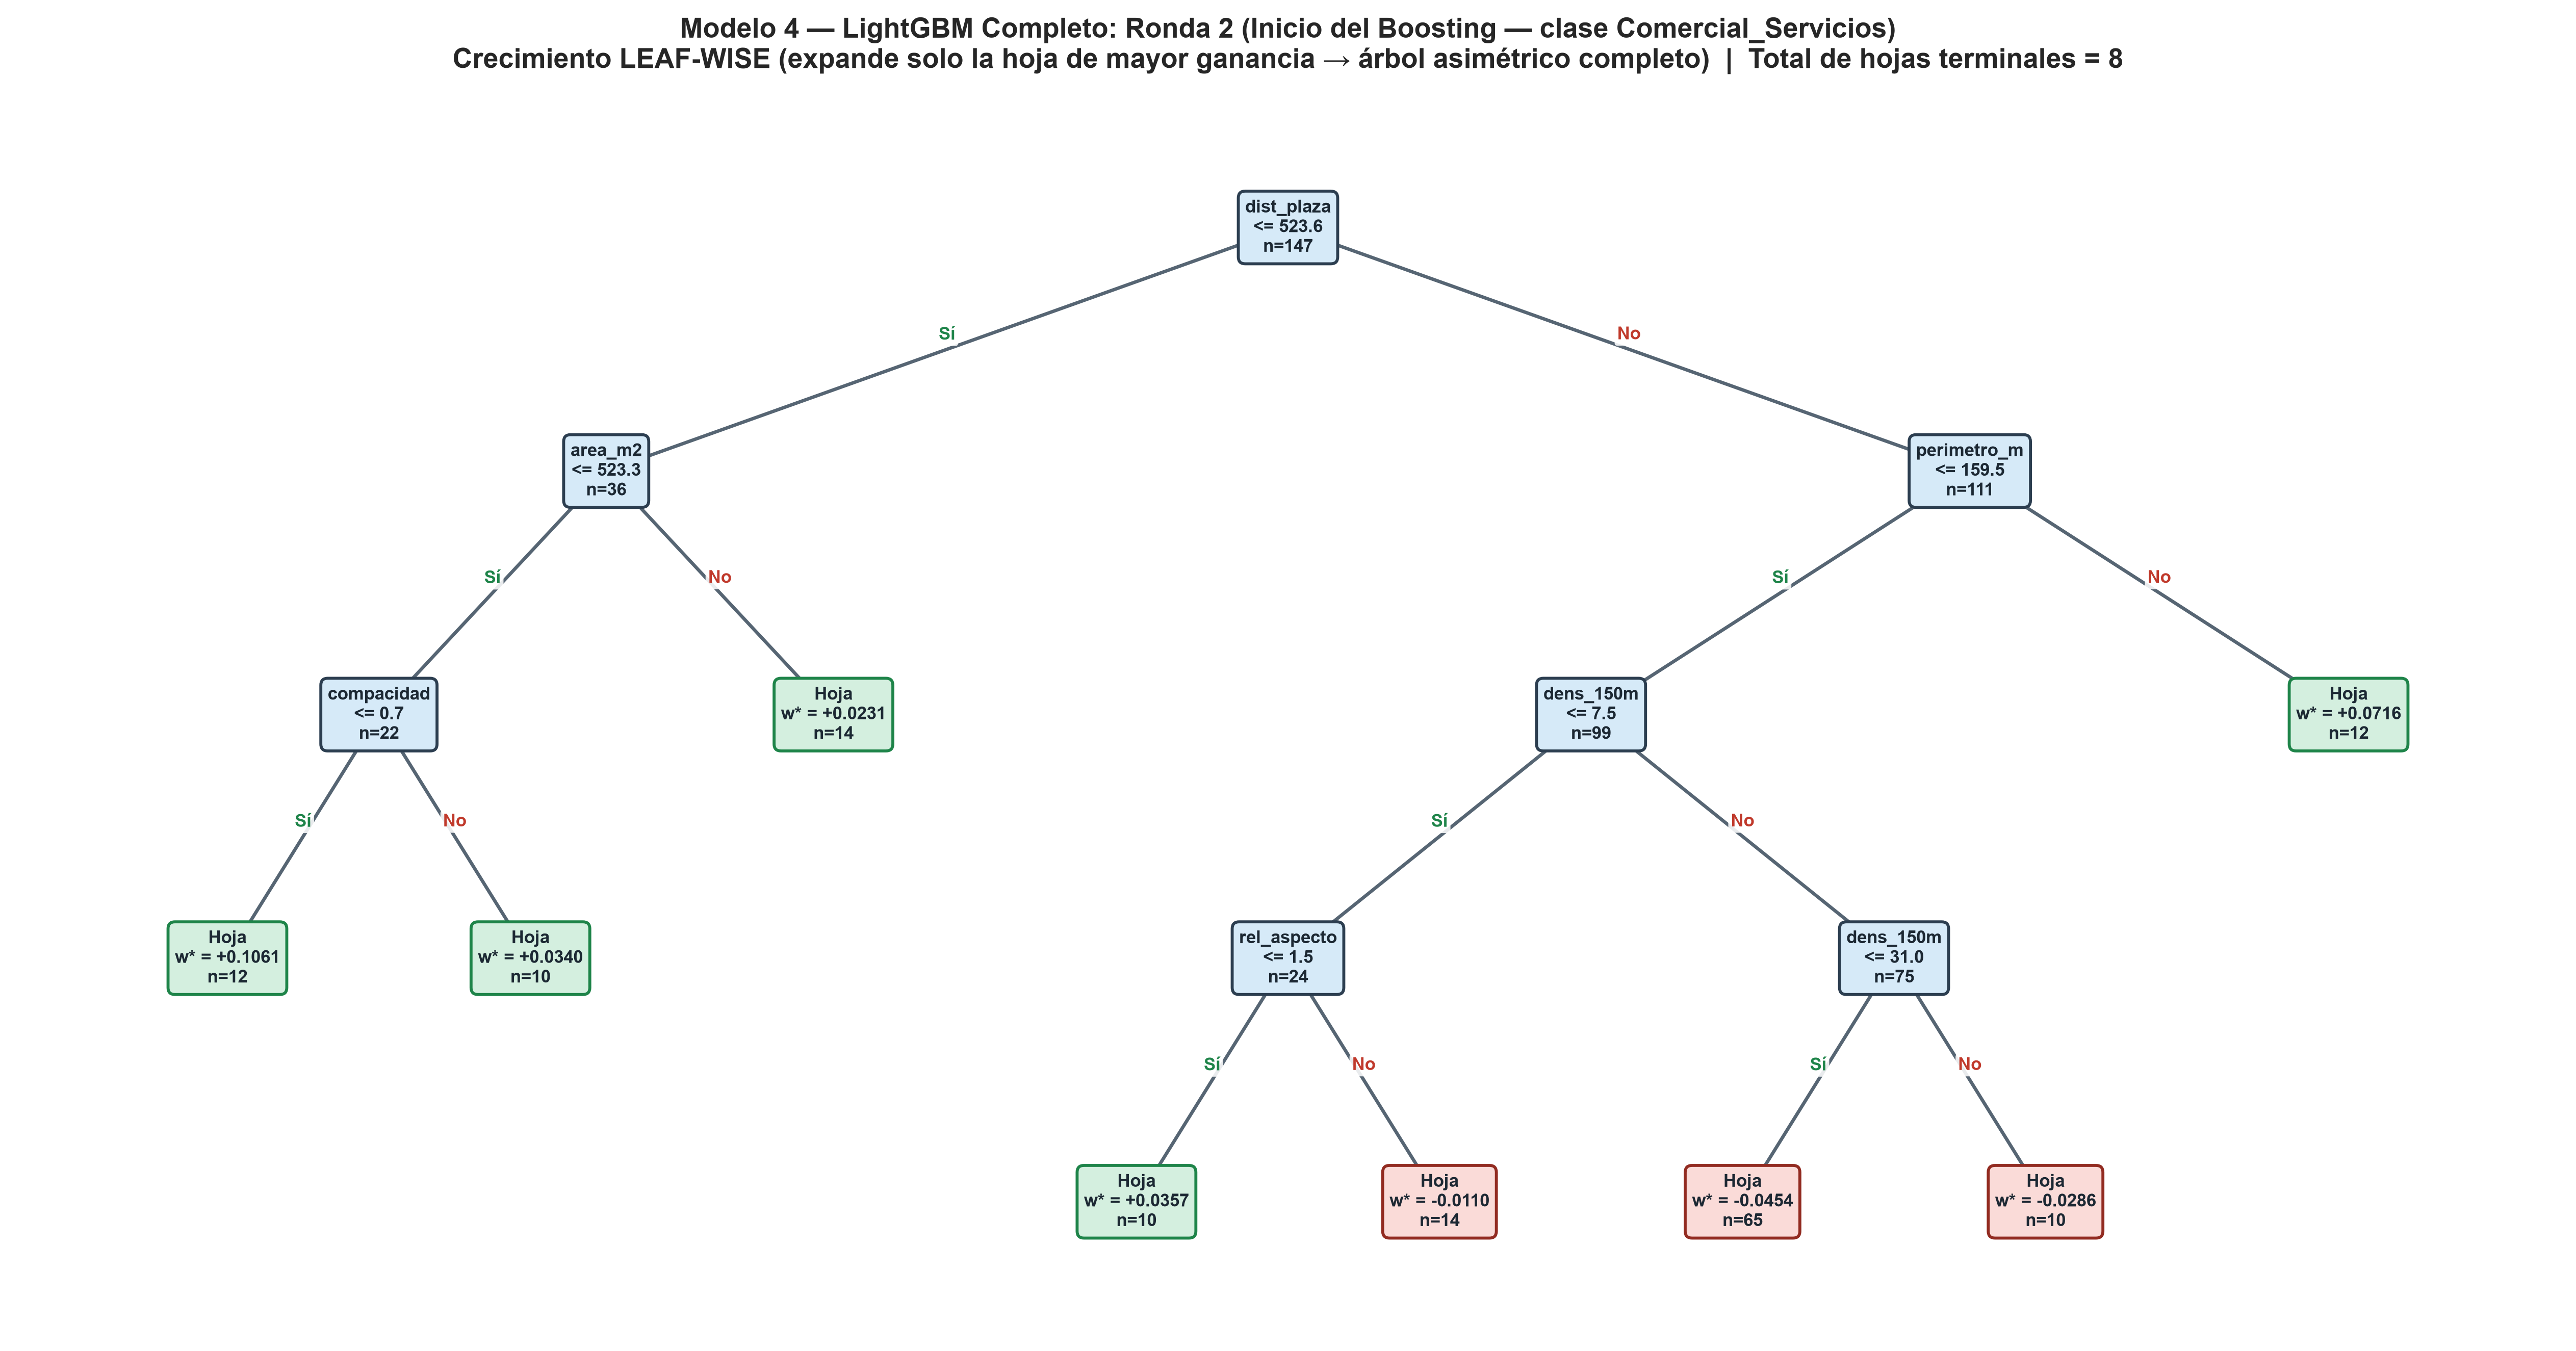
\includegraphics[width=0.92\textwidth]{figures/02_arbol_lightgbm_ronda2_completo.png}
    \caption{Árbol completo de \textbf{LightGBM} en la Ronda~2 (clase \texttt{Comercial\_Servicios}, $8$ hojas terminales): crecimiento asimétrico por hojas (\textit{leaf-wise}).}
    \label{fig:nb02_lgbm2}
\end{figure}

\begin{figure}[H]
    \centering
    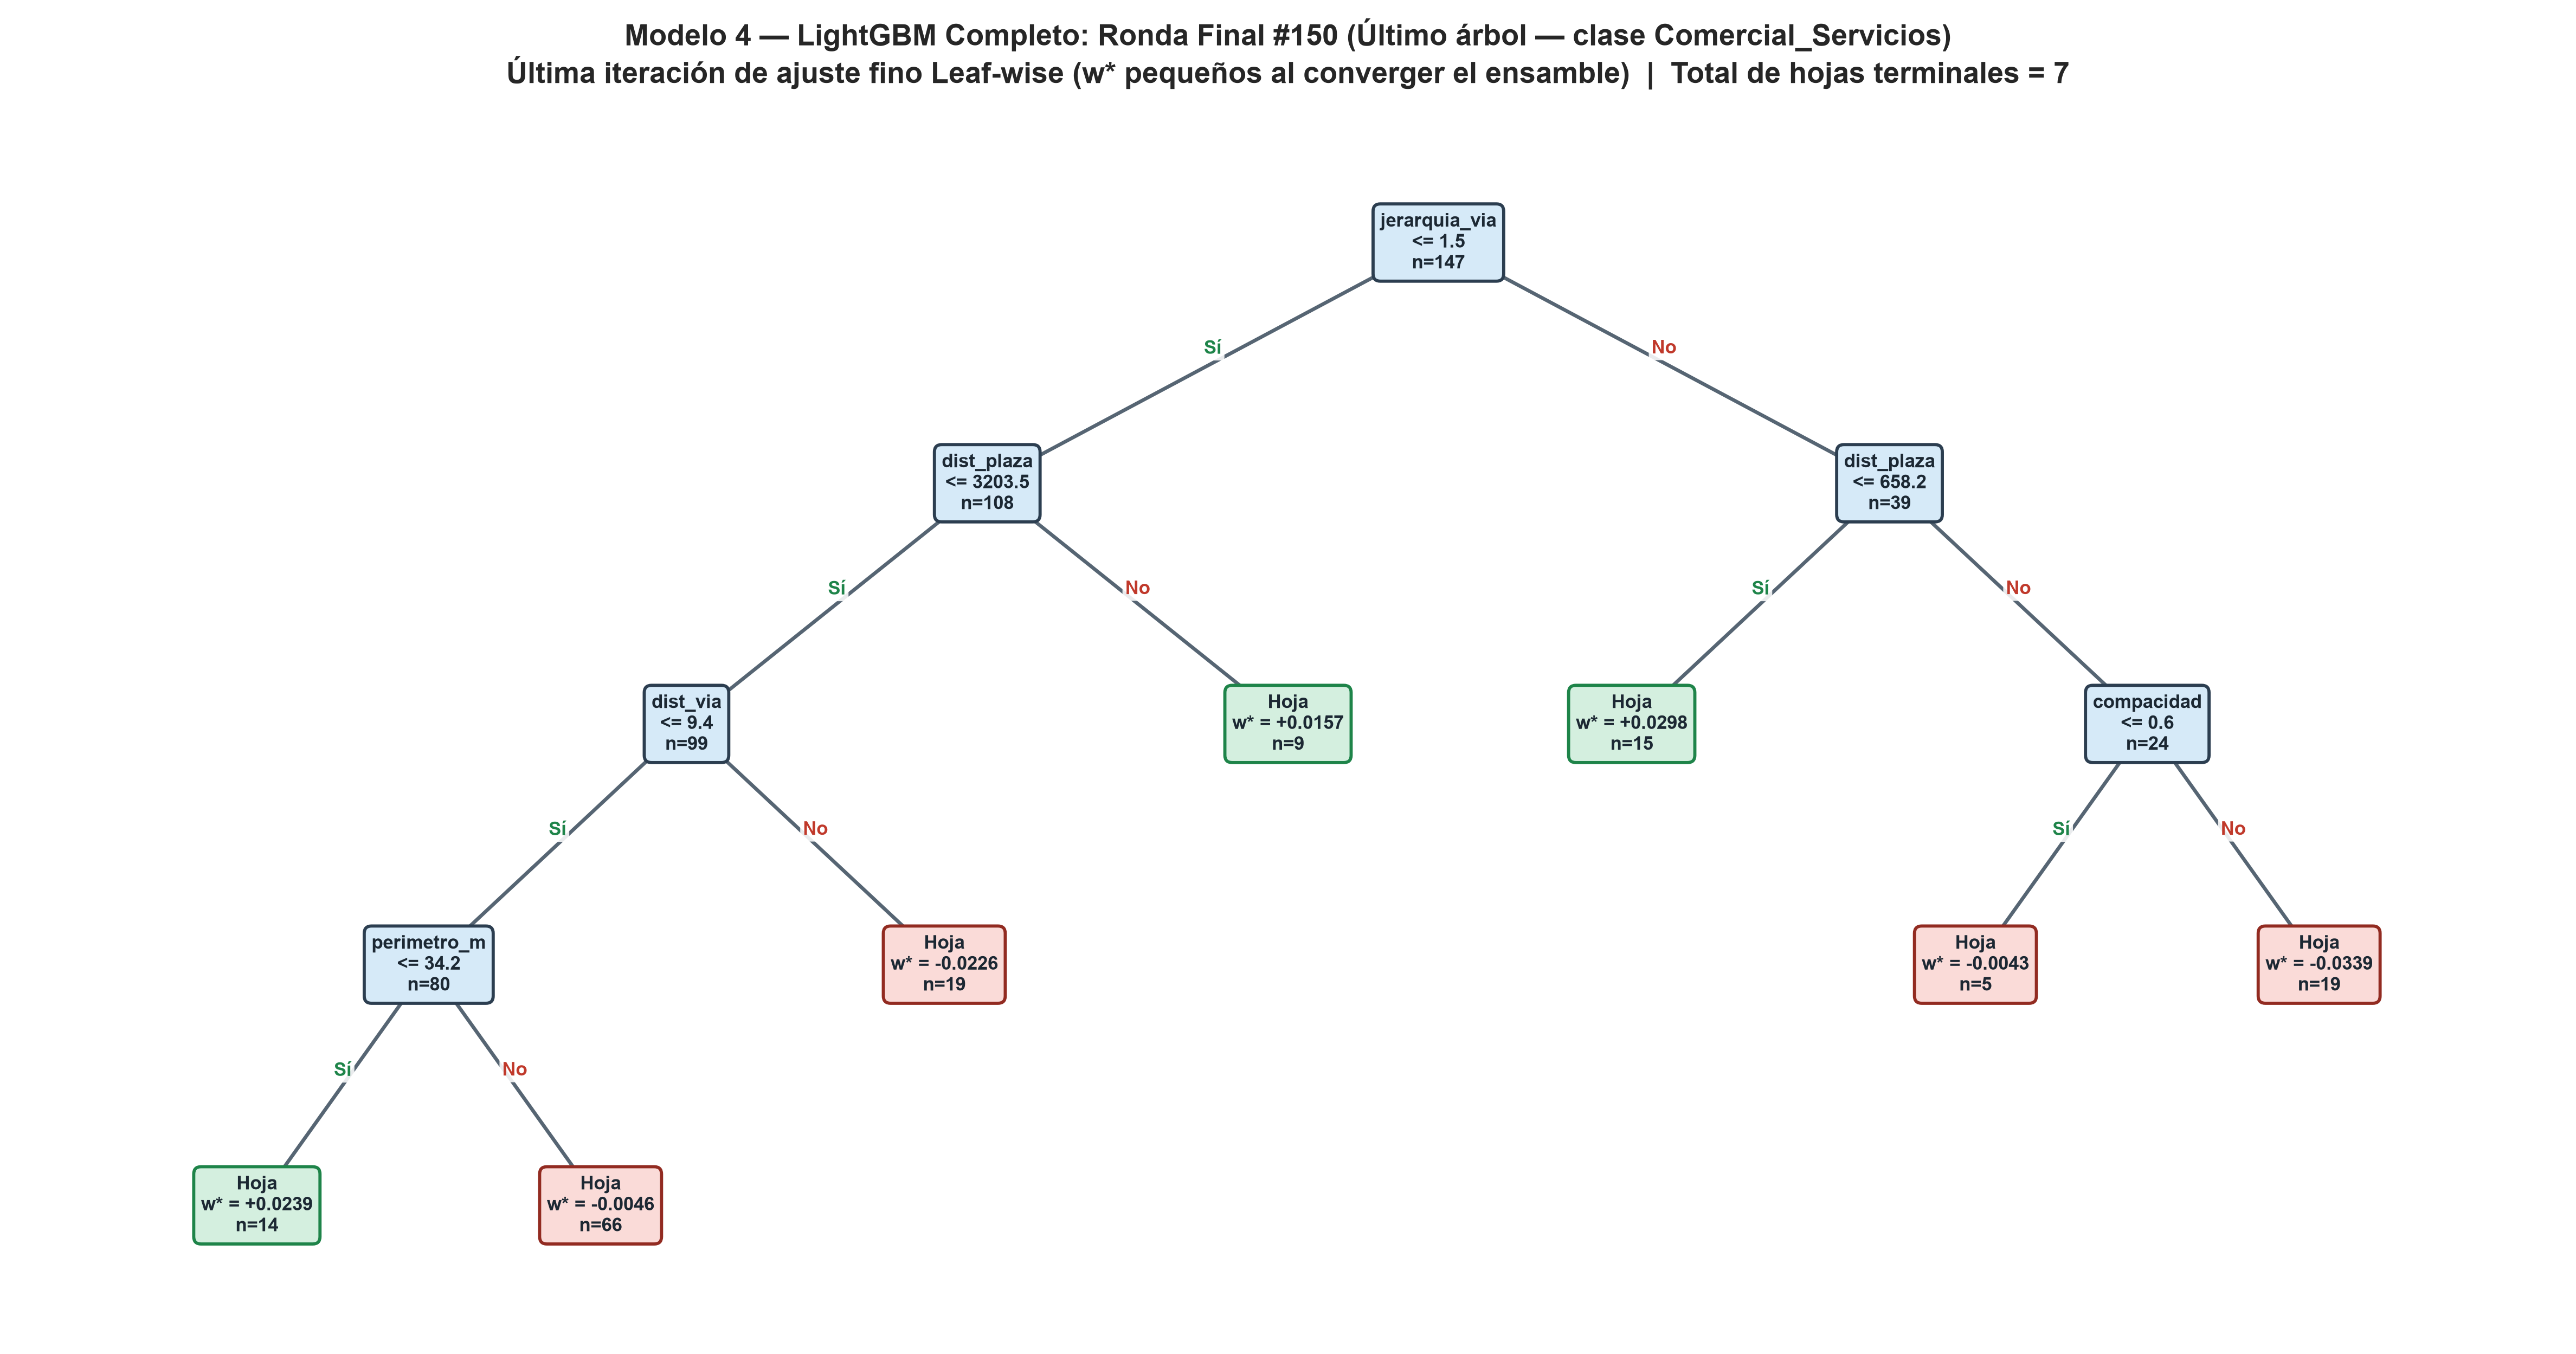
\includegraphics[width=0.88\textwidth]{figures/02_arbol_lightgbm_ronda150_completo.png}
    \caption{Árbol completo de \textbf{LightGBM} en la Ronda Final~\#150 ($7$ hojas terminales): última iteración de ajuste fino \textit{leaf-wise}.}
    \label{fig:nb02_lgbm150}
\end{figure}

\subsection{Matrices de Confusión e Importancia de Variables}

Para evaluar en qué clases acierta o se equivoca cada algoritmo durante el examen final ($20\%$ Test, $n = 37$ edificaciones), la Figura~\ref{fig:nb02_cm} presenta las cinco matrices de confusión lado a lado.

\begin{figure}[H]
    \centering
    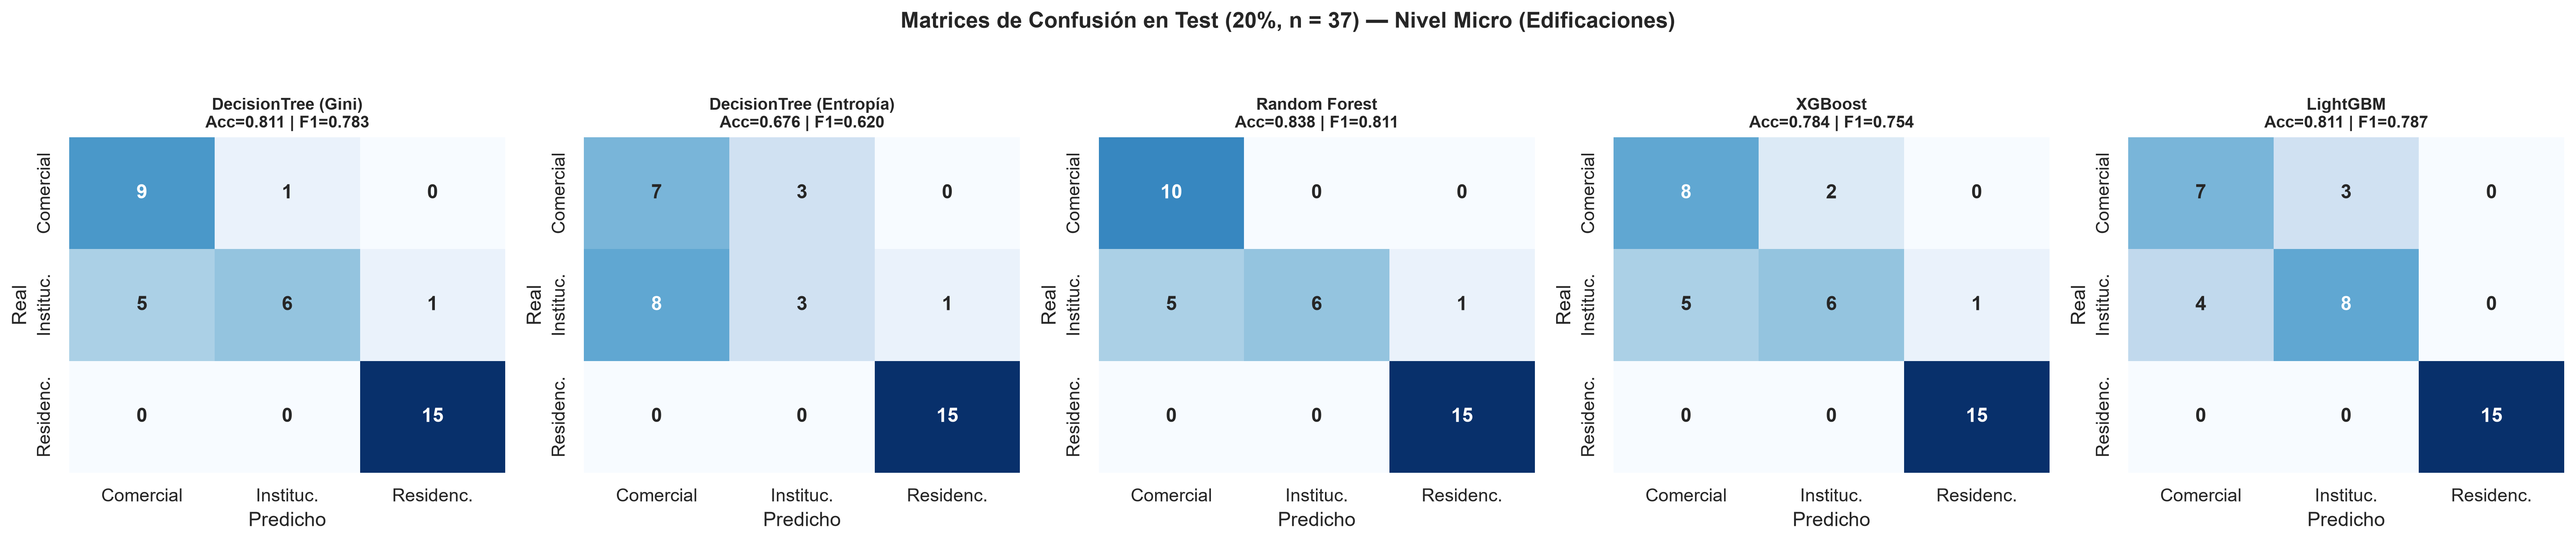
\includegraphics[width=0.99\textwidth]{figures/02_matrices_confusion_micro.png}
    \caption{Matrices de confusión en el conjunto de prueba ($20\%$, $n = 37$) para las cinco configuraciones del Nivel Micro.}
    \label{fig:nb02_cm}
\end{figure}

Complementariamente, la Figura~\ref{fig:nb02_fi} compara la importancia relativa normalizada de las $11$ variables entre las cuatro familias de modelos.

\begin{figure}[H]
    \centering
    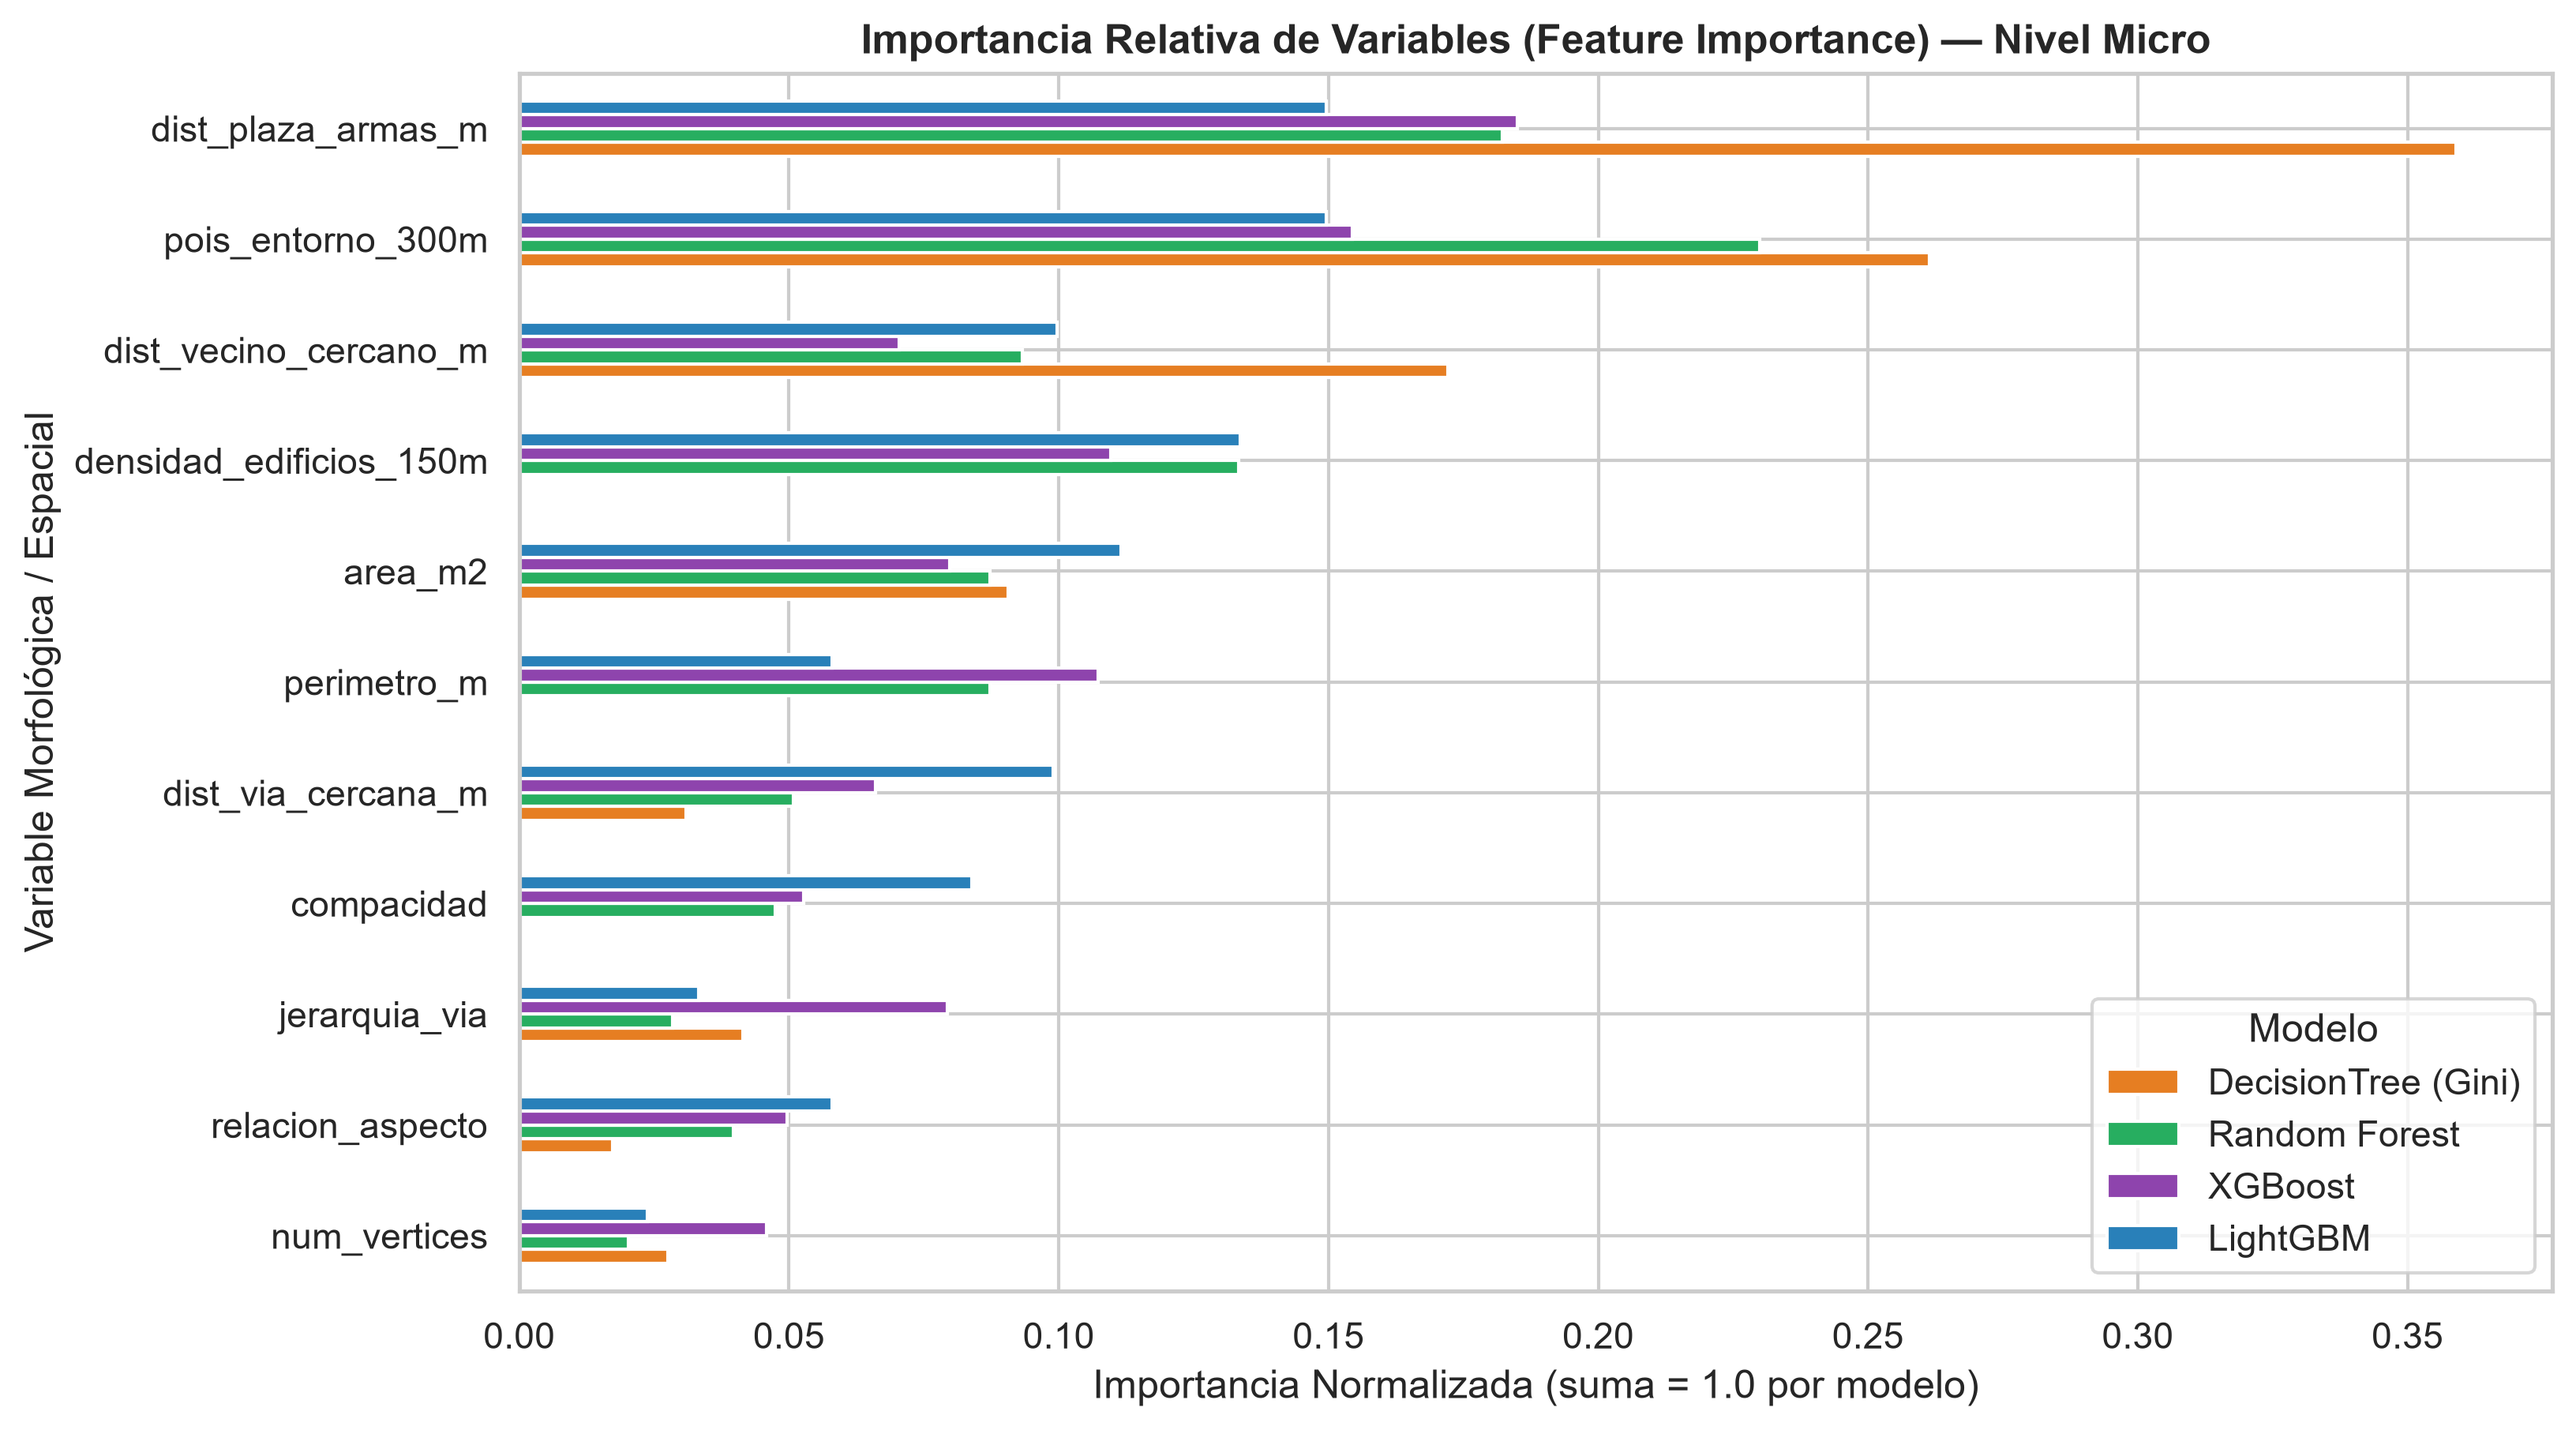
\includegraphics[width=0.88\textwidth]{figures/02_feature_importance_micro.png}
    \caption{Importancia relativa normalizada (\textit{Feature Importance}) de las $11$ variables morfológicas y espaciales en el Nivel Micro.}
    \label{fig:nb02_fi}
\end{figure}

\subsection{Reentrenamiento e Imputación Final}
  
Una vez completada la evaluación comparativa y seleccionado el modelo ganador según la métrica más robusta de generalización (\textbf{LightGBM}, $\text{CV-5 F1-Macro} = 0.7496$), ya no es necesario retener el $20\%$ de los datos etiquetados como examen. Por consiguiente, se instancia un modelo \textbf{LightGBM} nuevo con exactamente los mismos hiperparámetros validados y se entrena sobre el \textbf{100\% de las $184$ edificaciones verificadas} para maximizar la evidencia estadística disponible. Finalmente, este modelo reentrenado clasifica las \textbf{$468$ edificaciones sin etiqueta} de OpenStreetMap, integrando etiquetas verificadas y predichas en el archivo \texttt{puno\_buildings\_clasificados.geojson} (Tabla~\ref{tab:imputacion_micro}).

\begin{table}[H]
    \centering
    \caption{Distribución final de las $652$ edificaciones del Distrito de Puno tras la imputación con LightGBM.}
    \label{tab:imputacion_micro}
    \setlength{\tabcolsep}{7pt}
    \small
    \begin{adjustbox}{max width=\textwidth}
    \begin{tabular}{lrrr}
        \toprule
        \rowcolor{verdeHeader}
        \textcolor{white}{\textbf{Categoría Final (\texttt{clase\_final})}} & \textcolor{white}{\textbf{Verificado (OSM)}} & \textcolor{white}{\textbf{Predicho (ML — LightGBM)}} & \textcolor{white}{\textbf{Total Edificaciones}} \\
        \midrule
        \texttt{Institucional} & 60 & 227 & \textbf{287} ($44.0\%$) \\
        \rowcolor{verdeSuave!50}
        \texttt{Comercial\_Servicios} & 51 & 144 & \textbf{195} ($29.9\%$) \\
        \texttt{Residencial} & 73 & 97 & \textbf{170} ($26.1\%$) \\
        \midrule
        \rowcolor{verdeSuave}
        \textbf{Total Distrito de Puno} & \textbf{184} ($28.2\%$) & \textbf{468} ($71.8\%$) & \textbf{652} ($100.0\%$) \\
        \bottomrule
    \end{tabular}
    \end{adjustbox}
\end{table}

La Figura~\ref{fig:mapa_micro_folium} muestra la vista del mapa interactivo generado en Folium sobre el núcleo urbano de Puno.

\begin{figure}[H]
    \centering
    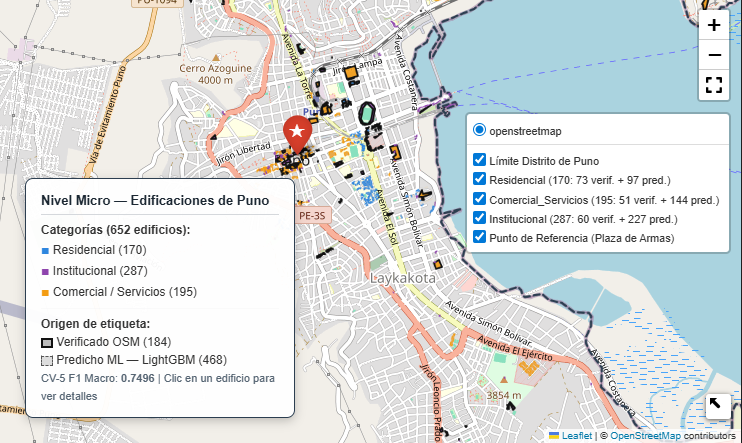
\includegraphics[width=0.96\textwidth]{figures/Nivel_Micro_Mapa.png}
    \caption{Mapa interactivo del Nivel Micro mostrando la clasificación de las $652$ edificaciones de Puno con distinción visual entre etiquetas verificadas en OSM (borde negro sólido) y predichas por LightGBM.}
    \label{fig:mapa_micro_folium}
\end{figure}


% ==============================================================================
% SECCIÓN 4: NIVEL MACRO — ZONIFICACIÓN URBANA (BASADO EN NB 03)
% ==============================================================================
\section{Nivel Macro: Zonificación y Uso de Suelo Urbano en el Distrito de Puno}
\label{sec:macro}

Esta sección desarrolla la clasificación territorial a escala \textbf{Macro (Zonificación y Uso de Suelo)} sobre el Distrito de Puno. A diferencia del Nivel Micro que evalúa cada edificio individual, aquí se analiza la estructura funcional de sectores completos de la ciudad integrando las edificaciones ya clasificadas junto con la red vial, el transporte, los servicios y la hidrografía del Lago Titicaca.

\subsection{Generación de la Grilla Espacial ($250\text{ m} \times 250\text{ m}$) y Etiquetado Verificable ($y$)}

Tal como se diagnosticó, OpenStreetMap presenta una desproporción geométrica severa en la capa \texttt{landuse} ($25$ polígonos de \texttt{residential} cubren $33.53\text{ km}^2$, mientras que $110$ polígonos de \texttt{grass} cubren solo $0.02\text{ km}^2$). Para construir una unidad espacial homogénea y estadísticamente justa, el polígono distrital de Puno fue dividido en una \textbf{cuadrícula regular de celdas de $250\text{ m} \times 250\text{ m}$} ($62{,}500\text{ m}^2 = 6.25\text{ hectáreas}$ por celda), obteniéndose $7{,}657$ celdas totales en el distrito.

De ese total se filtraron únicamente las \textbf{$2{,}100$ celdas activas} (aquellas que intersectan vías, edificaciones, POIs o polígonos de uso de suelo). Las etiquetas reales de la variable objetivo \textbf{\texttt{zona\_macro}} se extrajeron exclusivamente desde las capas poligonales (\texttt{puno\_landuse} y \texttt{puno\_pois\_a}), priorizando los usos específicos sobre la capa genérica residencial para evitar solapamientos:
\begin{enumerate}[leftmargin=0.85cm, itemsep=2pt]
    \item \textbf{\texttt{Equipamiento\_Productivo} ($149$ celdas; $14.8\%$):} Universidades, colegios, hospitales, mercados, industrias, comercio y comisarías.
    \item \textbf{\texttt{Areas\_Verdes\_Recreacion} ($127$ celdas; $12.6\%$):} Parques, losas deportivas (\texttt{pitch}), áreas verdes, recreación y cementerios.
    \item \textbf{\texttt{Rural\_Agricola\_Natural} ($167$ celdas; $16.6\%$):} Tierras agrícolas (\texttt{farmland}), matorrales (\texttt{scrub}), bosques y praderas.
    \item \textbf{\texttt{Urbano\_Residencial} ($566$ celdas; $56.1\%$):} Tejido habitacional consolidado de la ciudad.
\end{enumerate}

En total se obtuvieron \textbf{$1{,}009$ celdas verificadas} y \textbf{$1{,}091$ celdas activas sin etiqueta} de uso de suelo en OSM, que serán zonificadas al final por el modelo ganador (Figura~\ref{fig:nb03_grilla}).

\begin{figure}[H]
    \centering
    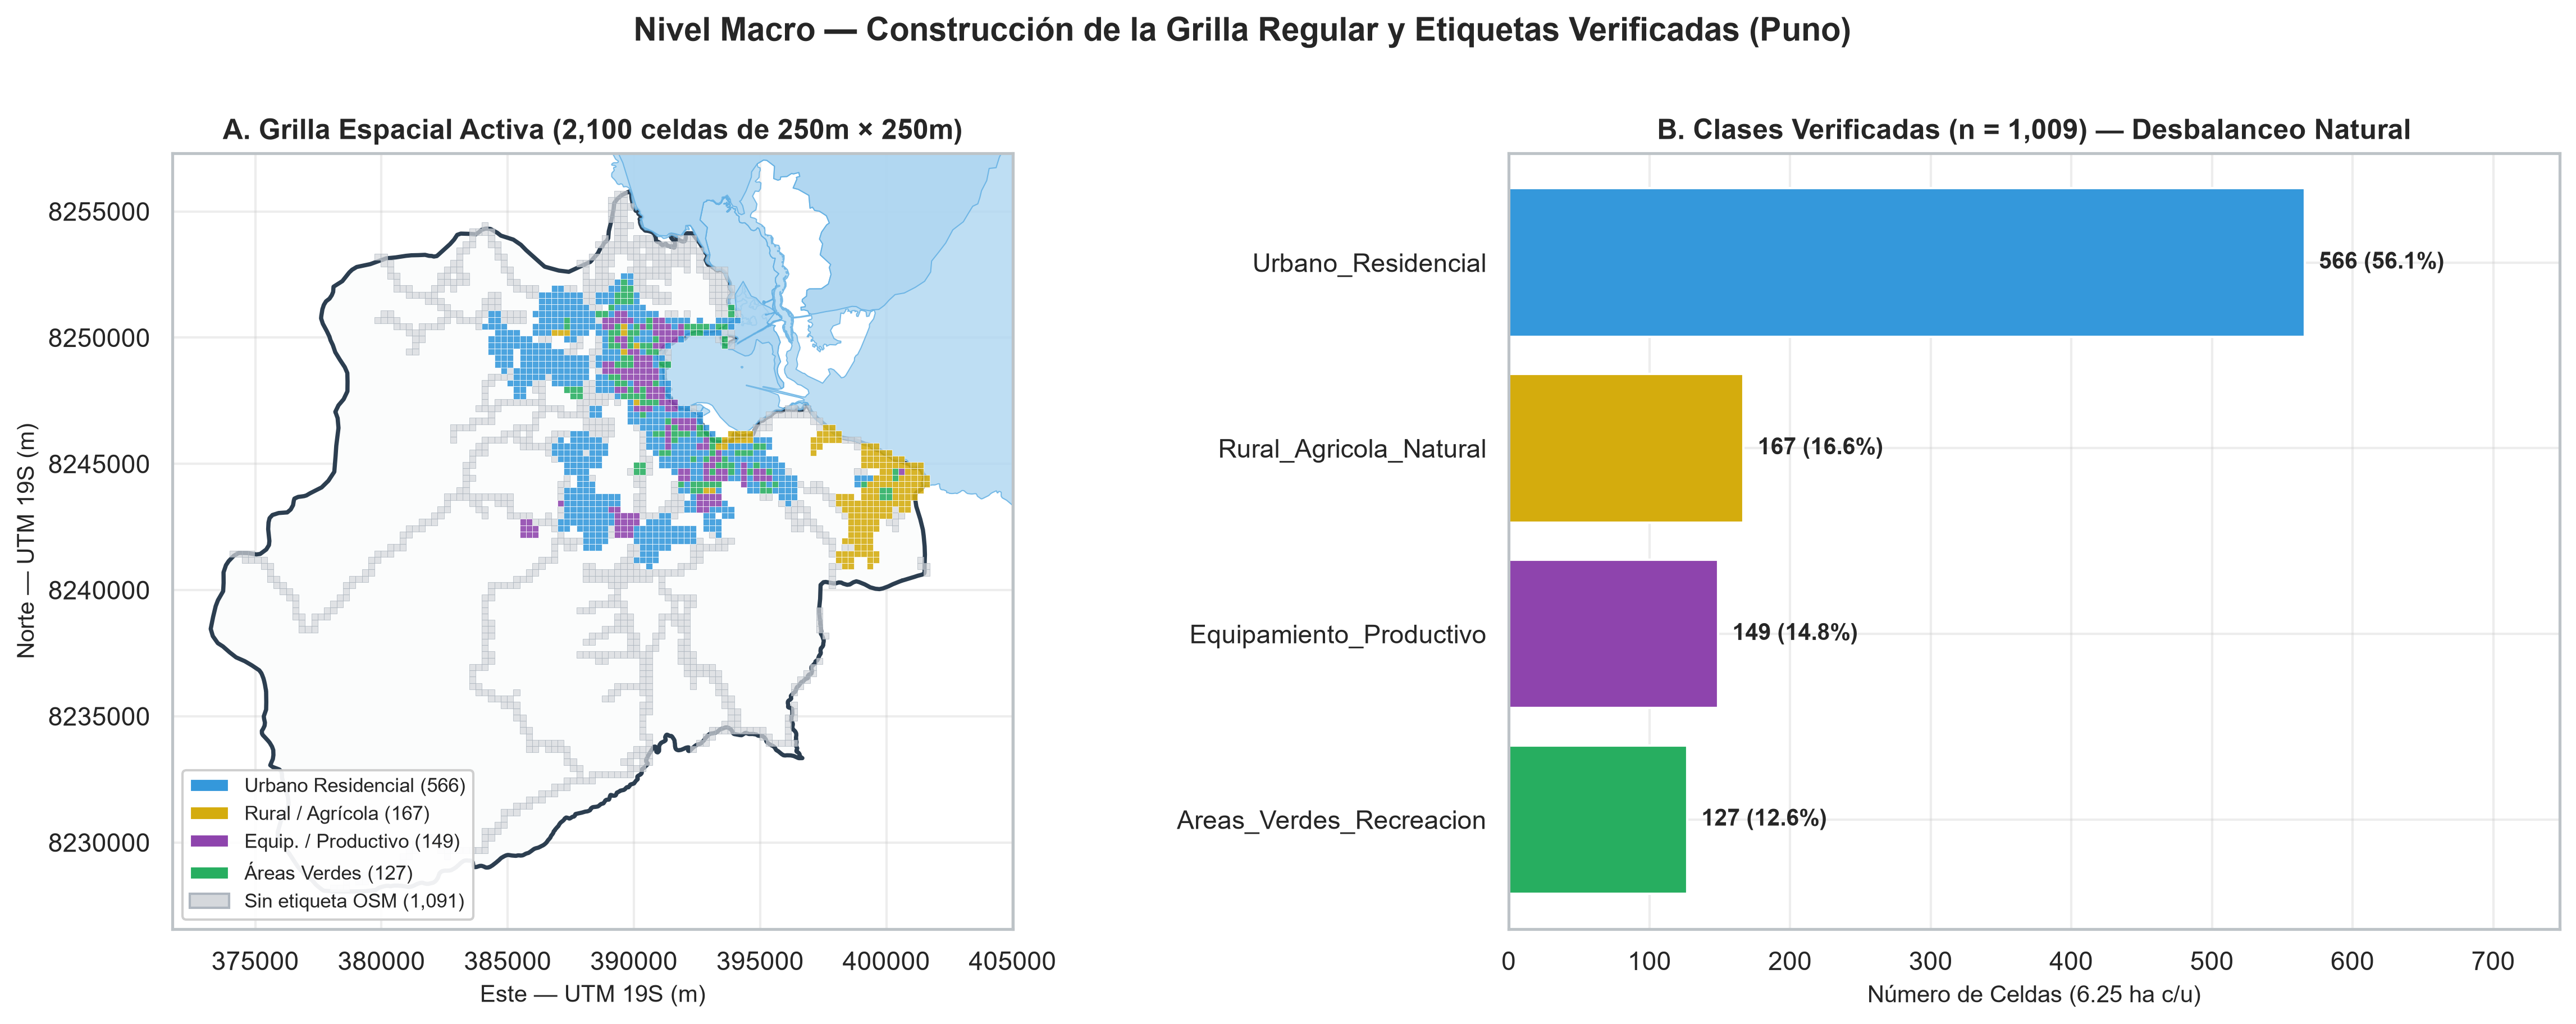
\includegraphics[width=0.99\textwidth]{figures/03_grilla_espacial_macro.png}
    \caption{Grilla espacial activa de $250\text{ m} \times 250\text{ m}$ en el Distrito de Puno ($2{,}100$ celdas) y distribución natural desbalanceada de las $1{,}009$ celdas verificadas en cuatro zonas.}
    \label{fig:nb03_grilla}
\end{figure}

\subsection{Ingeniería de 17 Variables Espaciales ($X$)}

Para describir cada celda de $250\text{ m} \times 250\text{ m}$ garantizando \textbf{cero fuga de datos} respecto a las etiquetas poligonales, se construyeron \textbf{$17$ variables predictoras numéricas ($X$)} a partir de cuatro fuentes independientes:
\begin{enumerate}[leftmargin=0.85cm, itemsep=2pt]
    \item \textbf{Agregación del Nivel Micro ($5$ variables):} integra las predicciones contabilizando número de edificios, porcentaje de área construida y número de edificios residenciales, comerciales e institucionales por celda.
    \item \textbf{Morfología y Densidad de la Red Vial ($5$ variables):} longitud total de vías dentro de la celda, número de tramos, proporción de vías arteriales, proporción de caminos rurales/peatonales y distancia a la vía principal más cercana.
    \item \textbf{Servicios Puntuales y Transporte con \texttt{cKDTree} ($4$ variables):} conteo de POIs dentro de la celda, densidad de POIs en radio de $500\text{ m}$, distancia al POI más cercano y distancia al paradero/terminal más próximo, calculadas eficientemente en $O(\log N)$.
    \item \textbf{Contexto Geográfico e Hídrico de Puno ($3$ variables):} distancia a la Plaza de Armas, distancia a la orilla del Lago Titicaca/cuerpos de agua y distancia a quebradas o ríos.
\end{enumerate}

La Tabla~\ref{tab:medianas_macro} resume las medianas de las variables más discriminantes en las $1{,}009$ celdas verificadas.

\begin{table}[H]
    \centering
    \caption{Medianas de las principales variables espaciales ($X$) por categoría de zonificación en el Nivel Macro ($n = 1{,}009$).}
    \label{tab:medianas_macro}
    \setlength{\tabcolsep}{4pt}
    \footnotesize
    \begin{adjustbox}{max width=\textwidth}
    \begin{tabular}{lrrrr}
        \toprule
        \rowcolor{verdeHeader}
        \textcolor{white}{\textbf{Variable Espacial ($X$)}} & \textcolor{white}{\textbf{Áreas Verdes}} & \textcolor{white}{\textbf{Equip./Prod.}} & \textcolor{white}{\textbf{Rural/Agríc.}} & \textcolor{white}{\textbf{Urb. Resid.}} \\
        \midrule
        \texttt{longitud\_vias\_m} (m) & 1{,}392.70 & 1{,}441.58 & 202.30 & 622.33 \\
        \rowcolor{verdeSuave!50}
        \texttt{num\_tramos\_via} & 14.00 & 14.00 & 1.00 & 6.00 \\
        \texttt{pct\_vias\_arteriales} & 0.03 & 0.10 & 0.00 & 0.00 \\
        \rowcolor{verdeSuave!50}
        \texttt{dist\_via\_principal\_m} (m) & 145.23 & 113.70 & 503.81 & 309.96 \\
        \texttt{num\_pois\_celda} & 1.00 & 1.00 & 0.00 & 0.00 \\
        \rowcolor{verdeSuave!50}
        \texttt{num\_pois\_500m} (\texttt{cKDTree}) & 10.00 & 11.00 & 0.00 & 0.00 \\
        \texttt{dist\_poi\_cercano\_m} (\texttt{cKDTree}, m) & 132.55 & 124.68 & 738.29 & 640.61 \\
        \rowcolor{verdeSuave!50}
        \texttt{dist\_transporte\_m} (\texttt{cKDTree}, m) & 838.84 & 865.95 & 7{,}090.38 & 2{,}196.42 \\
        \texttt{dist\_plaza\_armas\_m} (m) & 3{,}221.26 & 2{,}585.55 & 10{,}774.52 & 4{,}219.16 \\
        \rowcolor{verdeSuave!50}
        \texttt{dist\_lago\_agua\_m} (m) & 1{,}398.61 & 1{,}550.97 & 1{,}196.57 & 3{,}744.58 \\
        \texttt{dist\_quebrada\_rio\_m} (m) & 2{,}135.13 & 2{,}430.30 & 1{,}645.26 & 2{,}531.66 \\
        \bottomrule
    \end{tabular}
    \end{adjustbox}
\end{table}


\subsection{Validación (80\% Train / 20\% Test + 5-Fold CV)}

Manteniendo el mismo rigor metodológico del Nivel Micro, las $1{,}009$ celdas verificadas se dividieron estratificadamente en \textbf{80\% Entrenamiento ($807$ celdas)} y \textbf{20\% Prueba ($202$ celdas como examen final)}, combinadas con \textbf{Validación Cruzada Estratificada 5-Fold}, dejando las $1{,}091$ celdas sin etiqueta estrictamente apartadas para la imputación final (Figura~\ref{fig:nb03_flujo}).

Para compensar el desbalanceo de clases se incorporaron pesos inversamente proporcionales a la frecuencia.
\begin{equation}
    w_k = \frac{N}{K \cdot N_k}
    \label{eq:balanceo_macro}
\end{equation}
donde $N = 807$ es el tamaño de entrenamiento y $K = 4$ clases. Aplicando la ecuación~(\ref{eq:balanceo_macro}), los pesos exactos resultantes fueron: \texttt{Areas\_Verdes\_Recreacion} ($w = 1.978$), \texttt{Equipamiento\_Productivo} ($w = 1.695$), \texttt{Rural\_Agricola\_Natural} ($w = 1.517$) y \texttt{Urbano\_Residencial} ($w = 0.445$). Así, equivocarse en una celda de áreas verdes penaliza $4.4\times$ más que equivocarse en una celda residencial, obligando a los cuatro modelos a clasificar bien las cuatro zonas y evaluándolos con \textbf{F1-Score Macro} y \textbf{Balanced Accuracy}.

\begin{figure}[H]
    \centering
    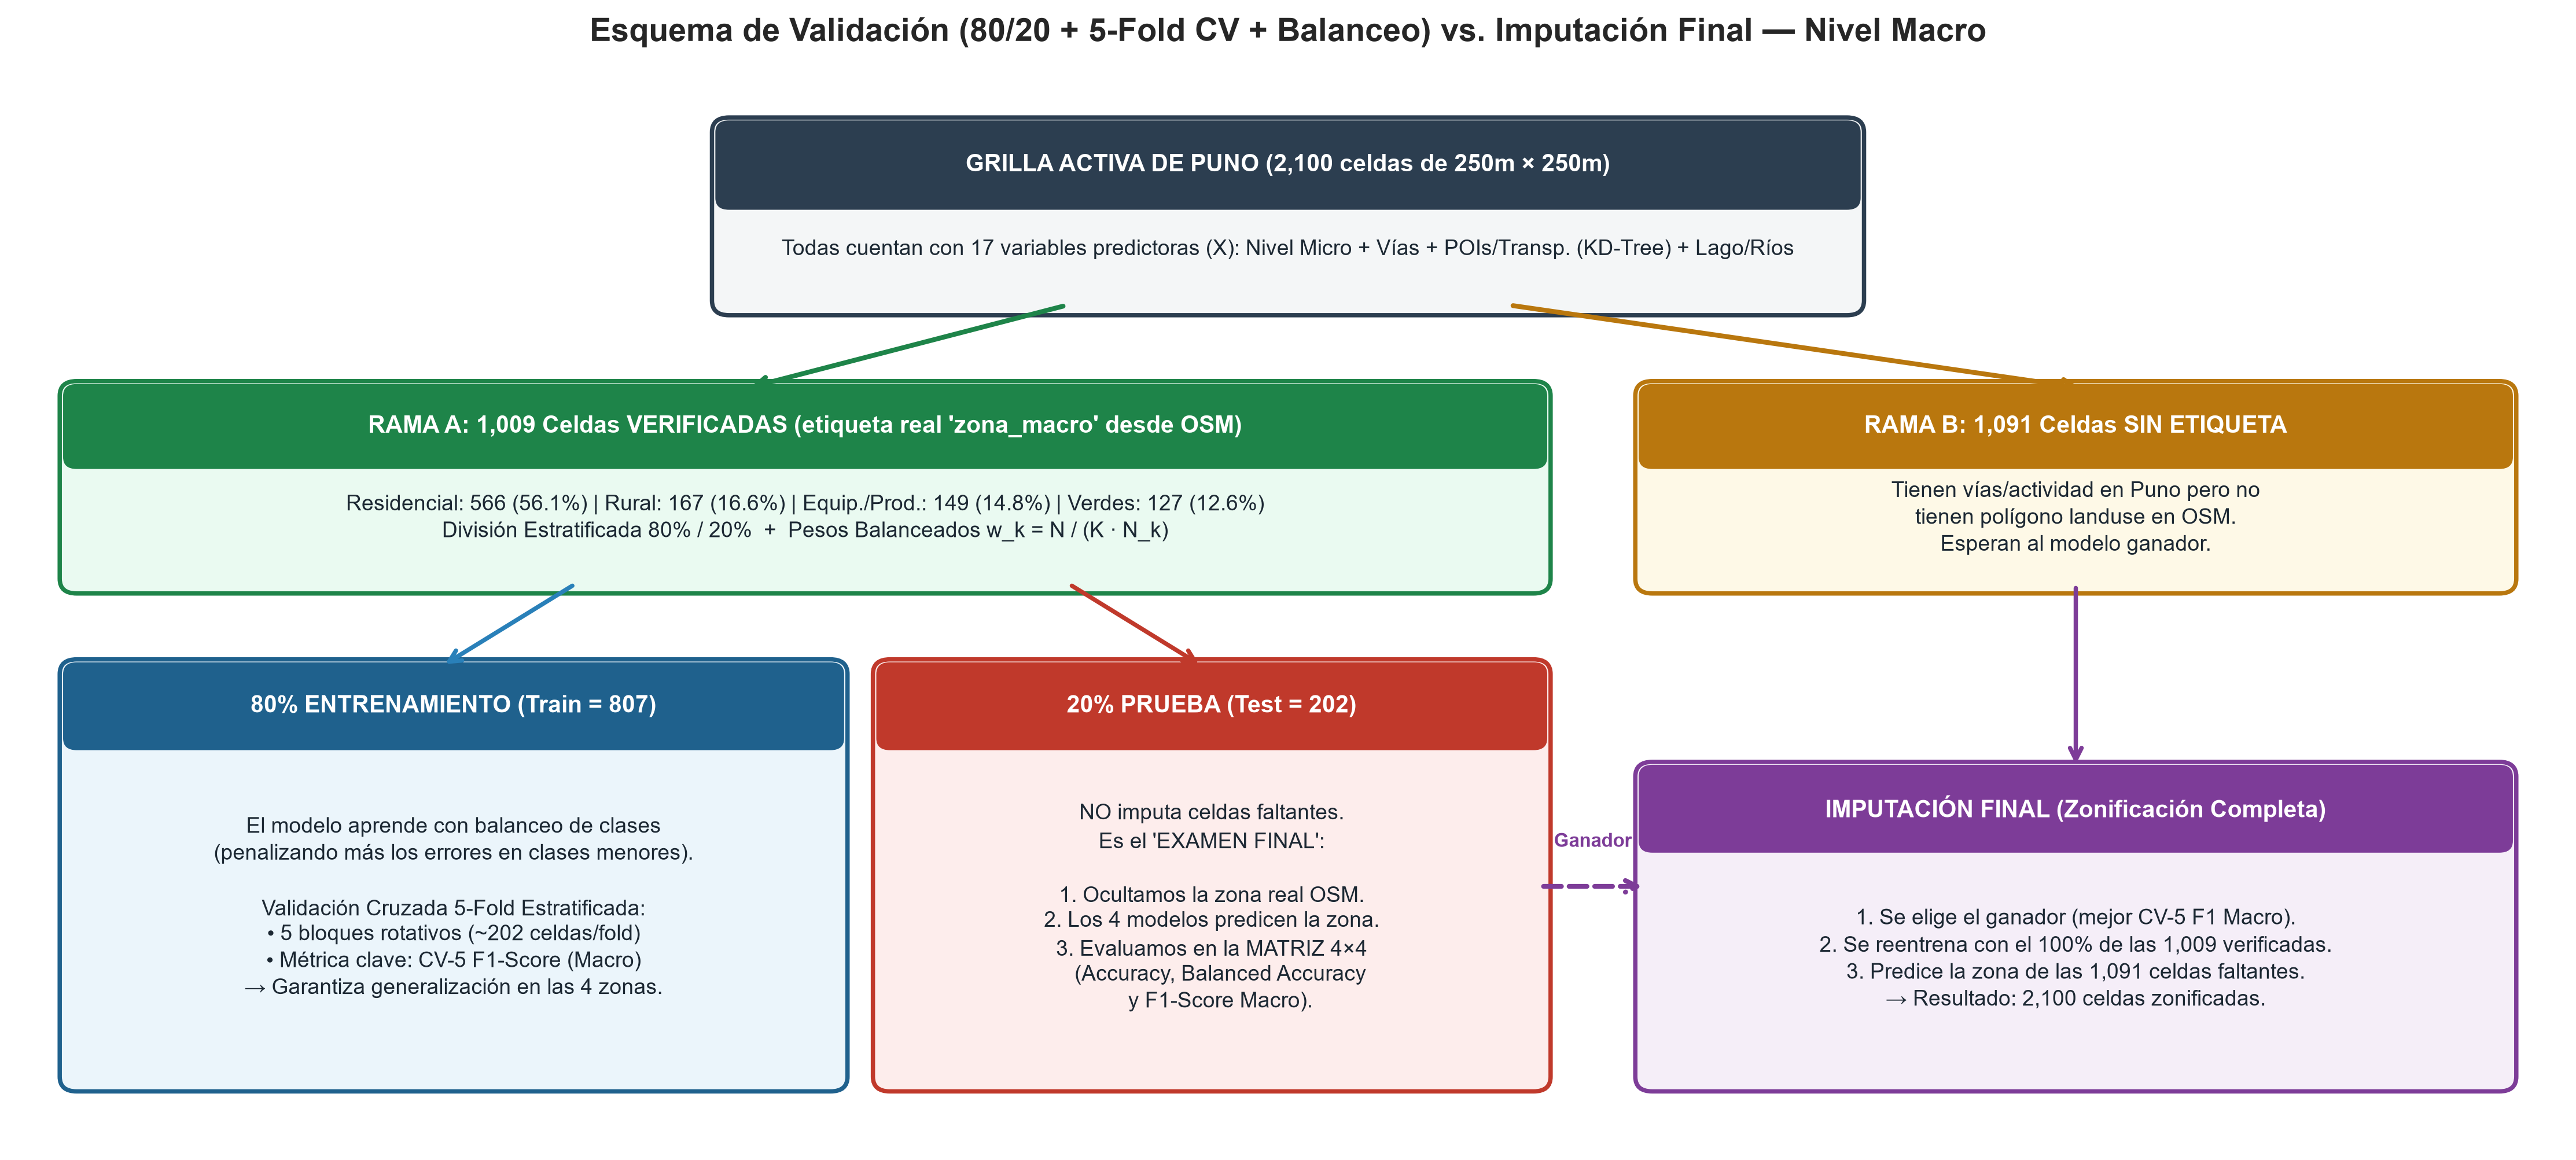
\includegraphics[width=0.98\textwidth]{figures/03_flujo_validacion_macro.png}
    \caption{Flujo de validación estratificada ($807$ entrenamiento, $202$ examen final y 5-Fold CV con balanceo de clases $w_k$) separado de la imputación final de las $1{,}091$ celdas sin etiqueta.}
    \label{fig:nb03_flujo}
\end{figure}

\subsection{Experimento de Poda y Comparativa de los 4 Modelos (Nivel Macro)}

Al variar \texttt{max\_depth} entre $2$ y $12$ en 5-Fold CV sobre el conjunto de entrenamiento (Figura~\ref{fig:nb03_poda}), tanto Gini como Entropía alcanzan su punto máximo de generalización exactamente en \textbf{\texttt{max\_depth = 6}} ($\text{F1} = 0.6033$ en Gini y $0.6014$ en Entropía). Con profundidades menores ($2\text{–}4$) existe subajuste ante la complejidad de $17$ variables y $4$ zonas; por encima de profundidad $6$, el desempeño desciende por sobreajuste.

\begin{figure}[H]
    \centering
    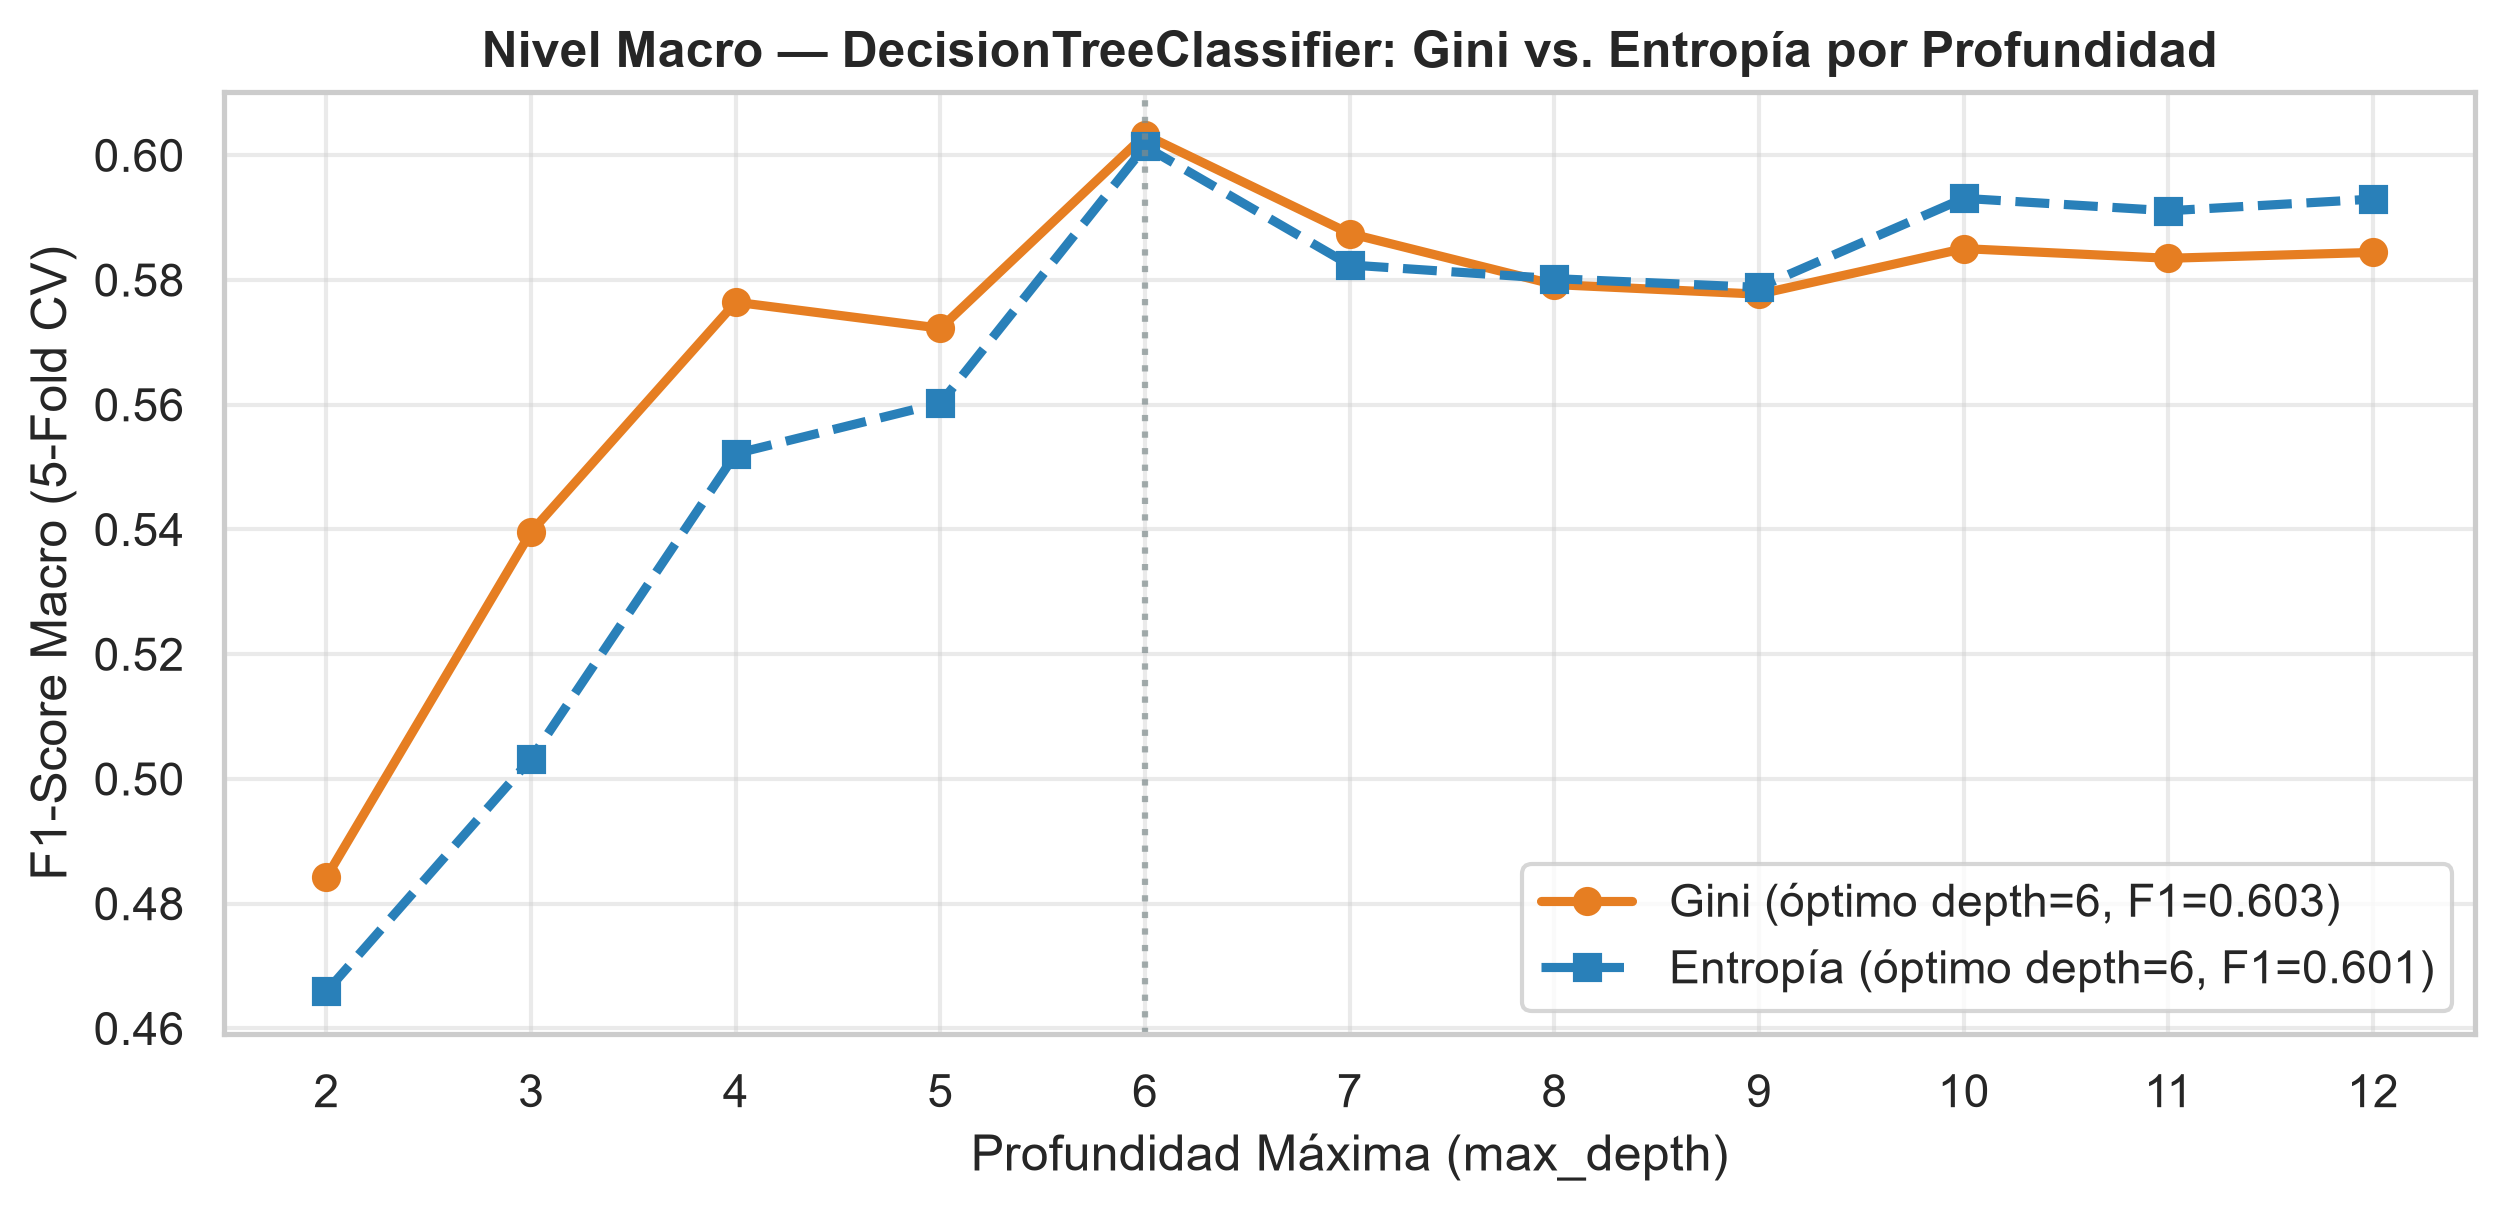
\includegraphics[width=0.82\textwidth]{figures/03_poda_gini_vs_entropia_macro.png}
    \caption{Experimento de poda (\texttt{max\_depth} de $2$ a $12$) comparando Gini y Entropía en el Nivel Macro mediante F1-Score Macro (5-Fold CV).}
    \label{fig:nb03_poda}
\end{figure}

La Tabla~\ref{tab:resultados_macro_nb03} presenta el benchmark completo de los cuatro modelos obligatorios (cinco configuraciones) evaluados en Test ($n=202$) y en Validación Cruzada 5-Fold.

\begin{table}[H]
    \centering
    \caption{Tabla comparativa de métricas y tiempo de entrenamiento de los 4 modelos (5 configuraciones) — Nivel Macro.}
    \label{tab:resultados_macro_nb03}
    \setlength{\tabcolsep}{3.5pt}
    \footnotesize
    \begin{adjustbox}{max width=\textwidth}
    \begin{tabular}{lcccccccc}
        \toprule
        \rowcolor{verdeHeader}
        \textcolor{white}{\textbf{Modelo}} & \textcolor{white}{\textbf{Test Acc}} & \textcolor{white}{\textbf{Bal. Acc}} & \textcolor{white}{\textbf{Prec (M)}} & \textcolor{white}{\textbf{Rec (M)}} & \textcolor{white}{\textbf{Test F1 (M)}} & \textcolor{white}{\textbf{CV-5 Acc}} & \textcolor{white}{\textbf{CV-5 F1 (M)}} & \textcolor{white}{\textbf{Tiempo (ms)}} \\
        \midrule
        \textbf{Random Forest} \textit{(Ganador CV)} & 0.7426 & 0.7023 & 0.6792 & 0.7023 & 0.6803 & 0.7681 & \textbf{0.6980} & 475.37 \\
        \rowcolor{verdeSuave!50}
        \textbf{XGBoost} \textit{(Ganador Test)} & \textbf{0.7772} & \textbf{0.7189} & \textbf{0.7065} & \textbf{0.7189} & \textbf{0.7120} & \textbf{0.7760} & 0.6977 & 733.07 \\
        LightGBM & 0.7574 & 0.6728 & 0.6619 & 0.6728 & 0.6670 & 0.7691 & 0.6767 & 310.12 \\
        \rowcolor{verdeSuave!50}
        DecisionTree (Gini) & 0.6535 & 0.6221 & 0.6039 & 0.6221 & 0.5996 & 0.6809 & 0.6318 & \textbf{5.20} \\
        DecisionTree (Entropía) & 0.6634 & 0.6205 & 0.5806 & 0.6205 & 0.5841 & 0.6671 & 0.5999 & 7.92 \\
        \bottomrule
    \end{tabular}
    \end{adjustbox}
\end{table}


\subsection{Visualización Completa de los Árboles en los 4 Modelos (Nivel Macro)}

\subsubsection{Modelos 1A y 1B — \texttt{DecisionTreeClassifier} (Gini y Entropía Completos)}

\begin{figure}[H]
    \centering
    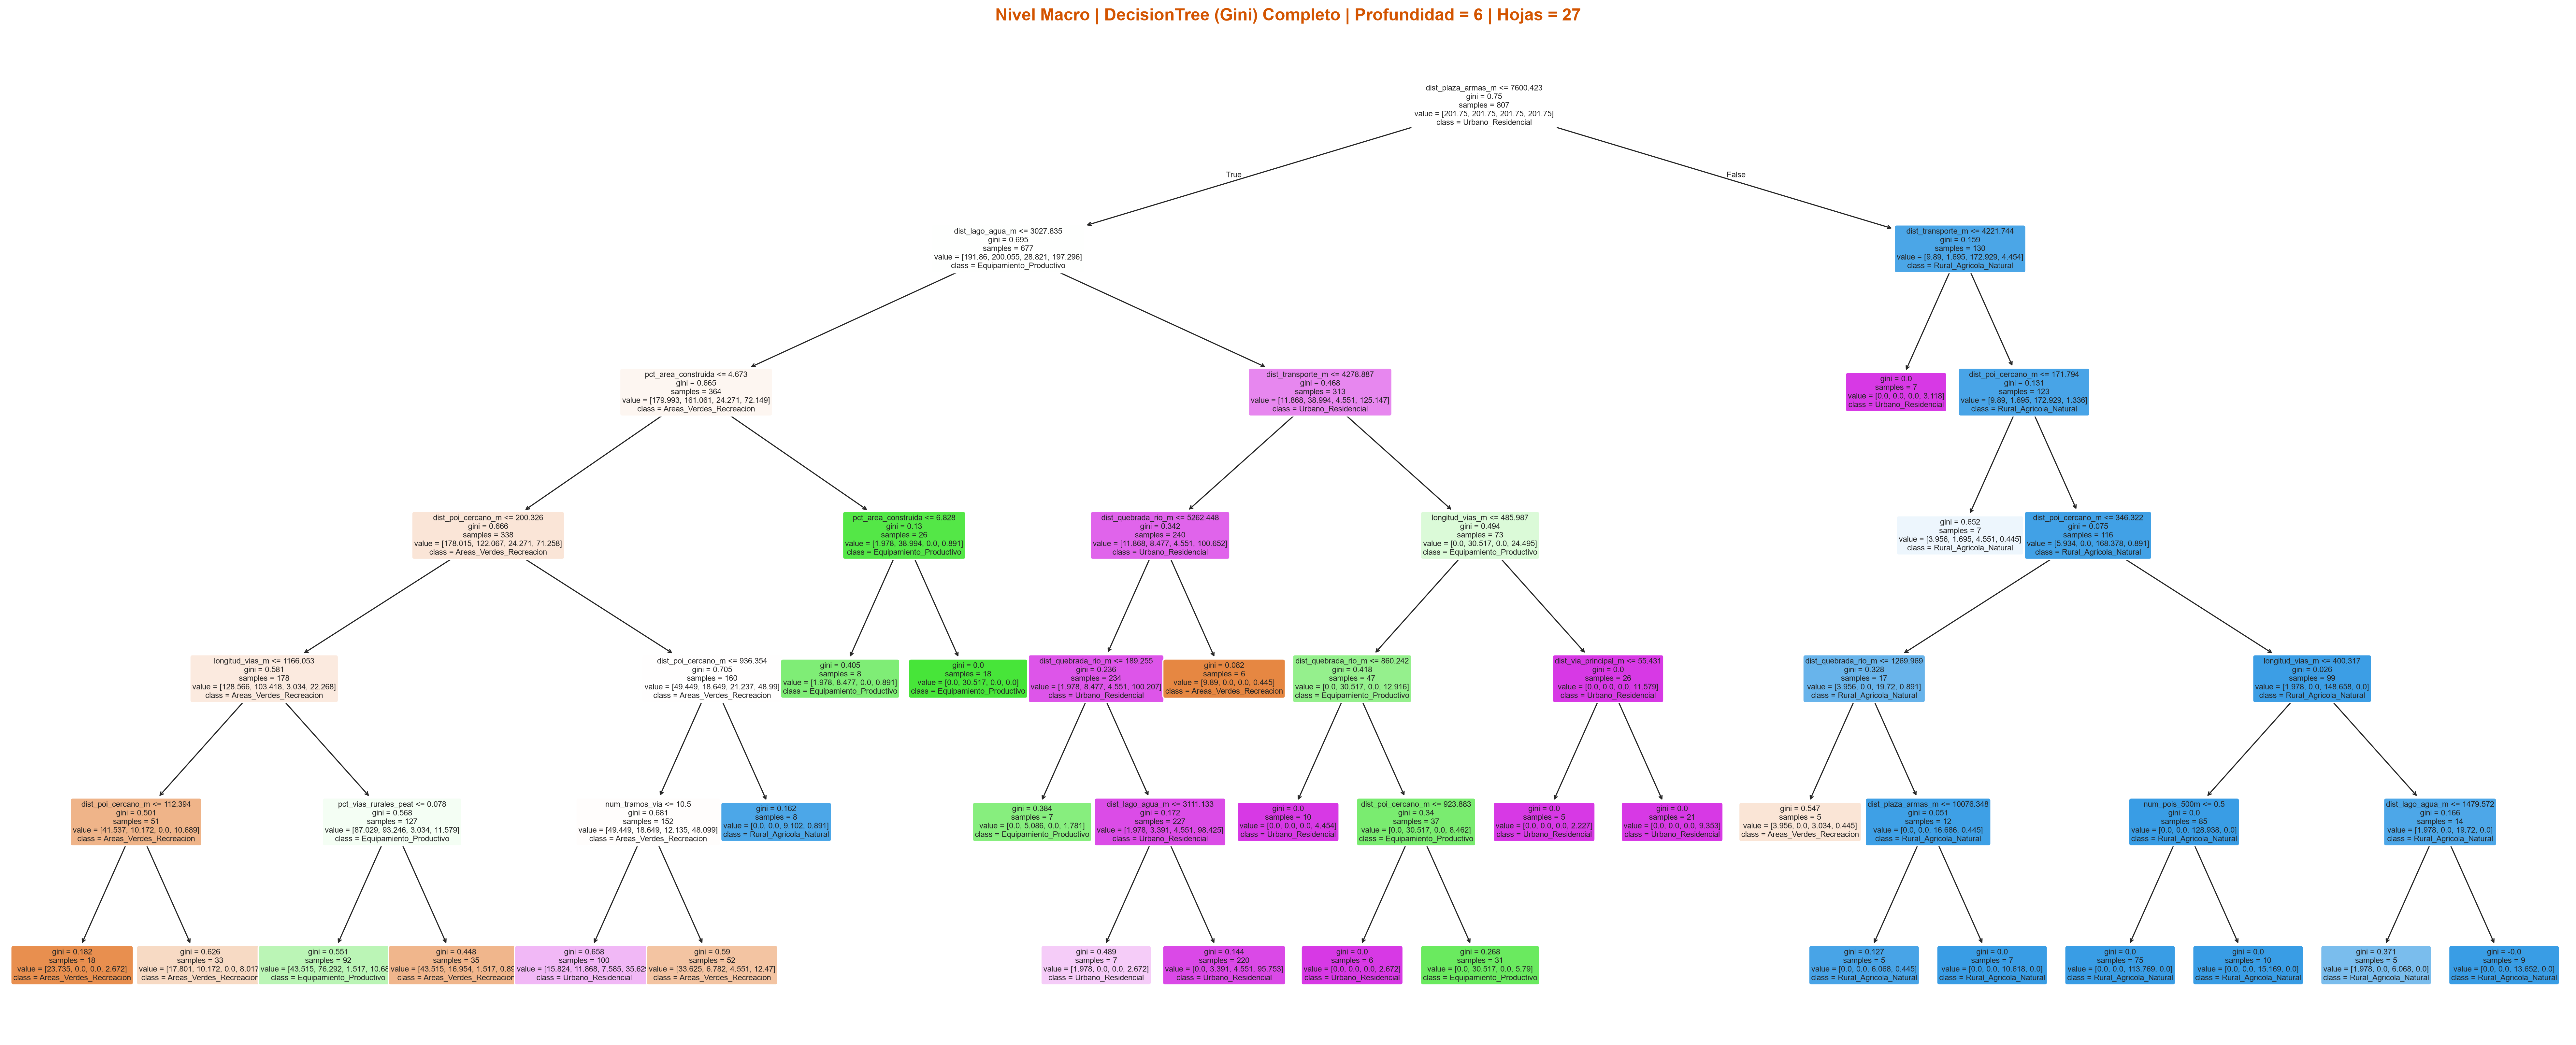
\includegraphics[width=0.99\textwidth]{figures/03_arbol_gini_completo.png}
    \caption{Árbol completo de \texttt{DecisionTreeClassifier (Gini)} en el Nivel Macro (profundidad $= 6$, $27$ hojas terminales).}
    \label{fig:nb03_gini}
\end{figure}

\begin{figure}[H]
    \centering
    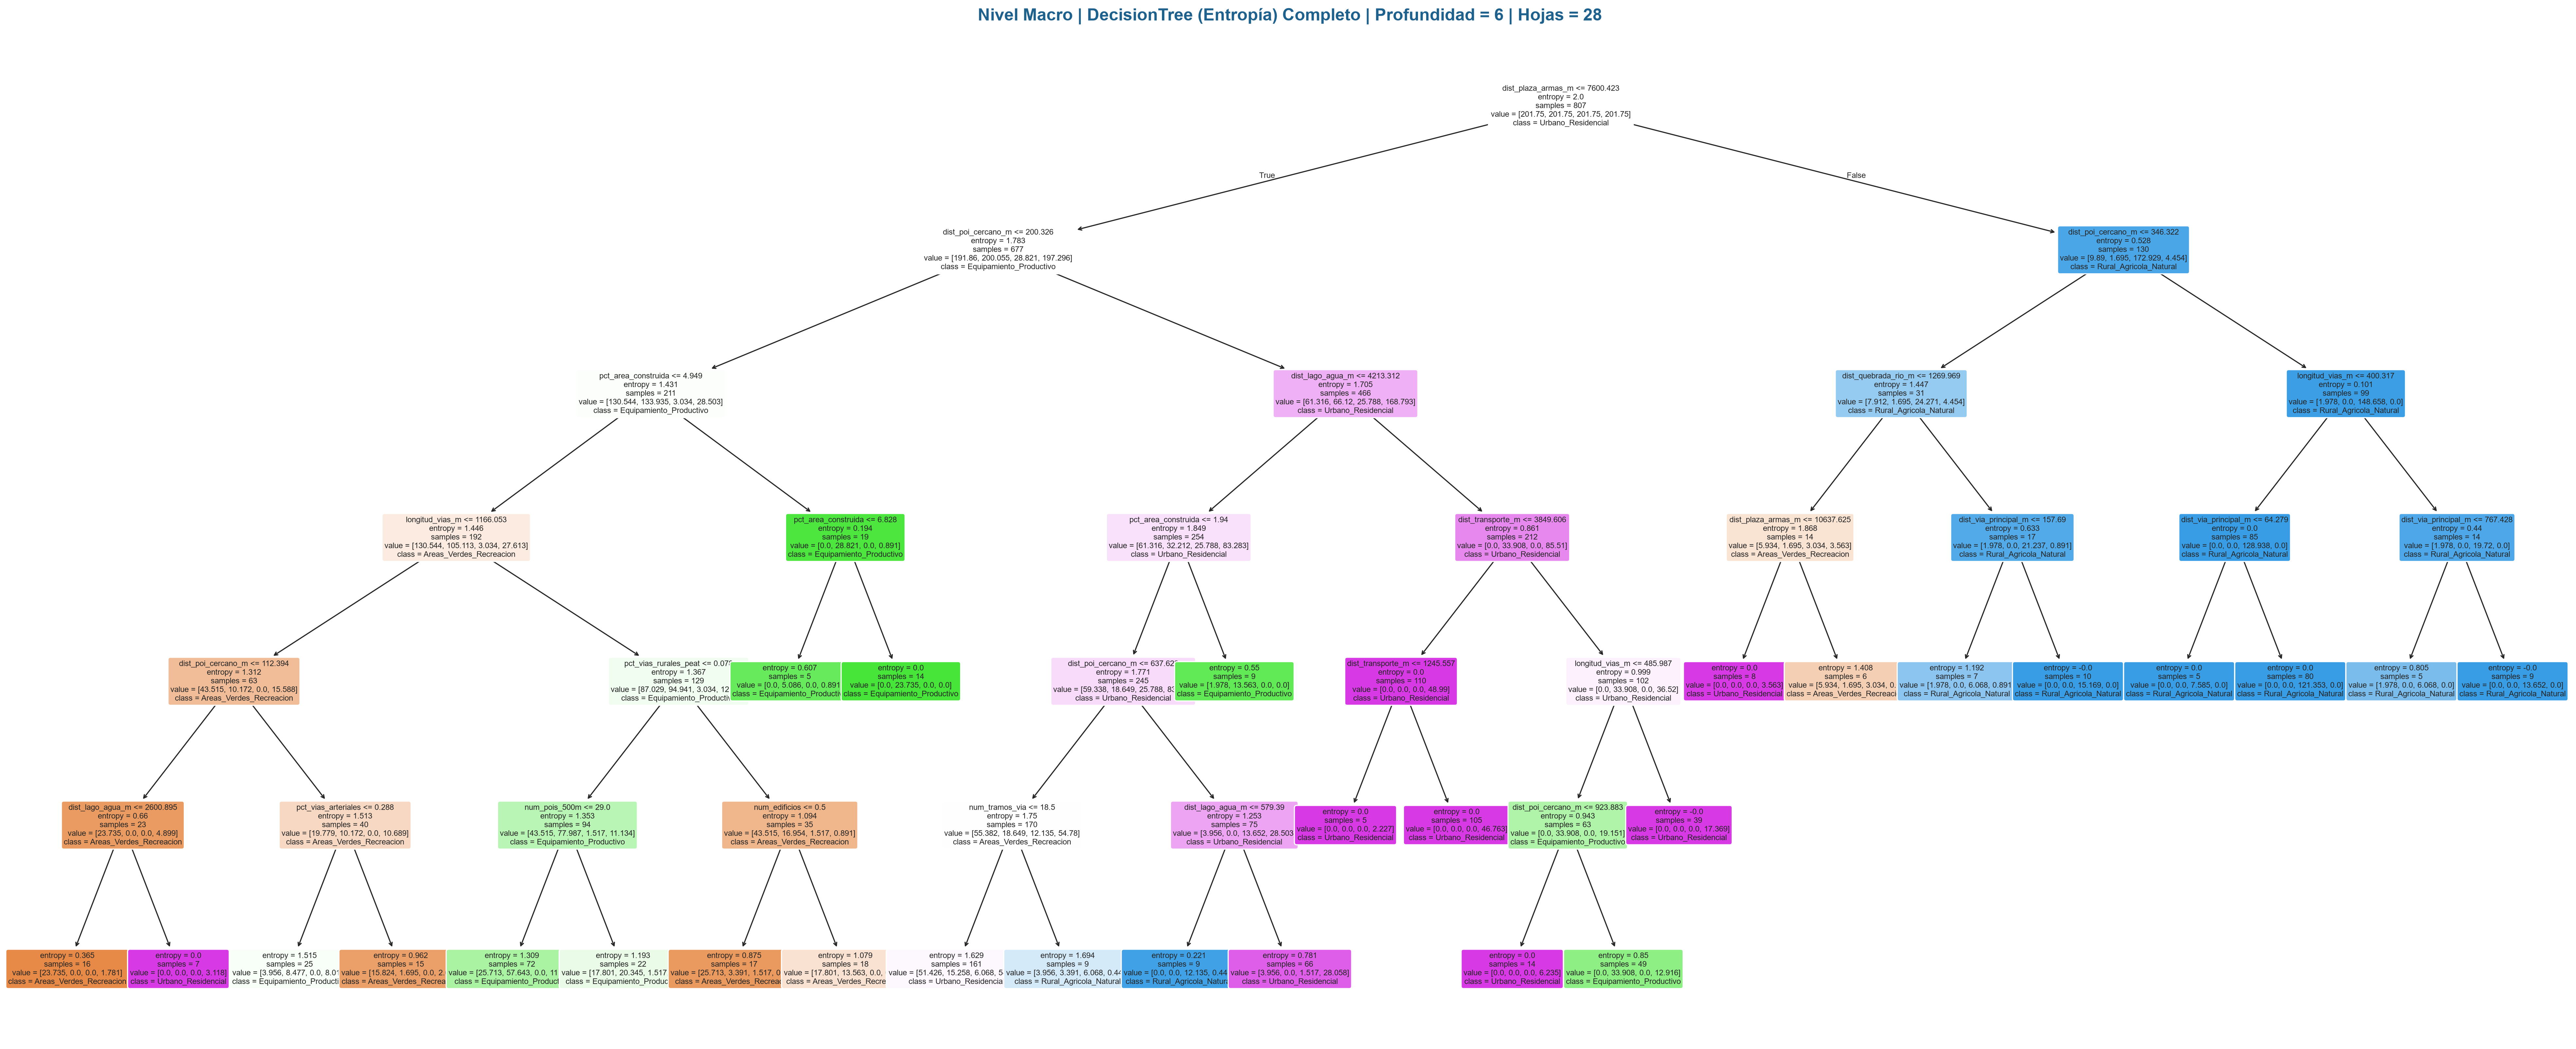
\includegraphics[width=0.99\textwidth]{figures/03_arbol_entropia_completo.png}
    \caption{Árbol completo de \texttt{DecisionTreeClassifier (Entropía)} en el Nivel Macro (profundidad $= 6$, $28$ hojas terminales).}
    \label{fig:nb03_entropia}
\end{figure}

\subsubsection{Modelo 2 — \texttt{RandomForestClassifier} (\textit{Bagging}): Árbol \#1 y Árbol \#250 Completos}

En el Nivel Macro, Random Forest entrena \textbf{$250$ árboles independientes en paralelo} con \texttt{max\_depth = 12} para capturar las fronteras espaciales entre las cuatro zonas. Las Figuras~\ref{fig:nb03_rf1} y~\ref{fig:nb03_rf250} muestran completos el primer árbol (\#1) y el último árbol (\#250) del bosque.

\begin{figure}[H]
    \centering
    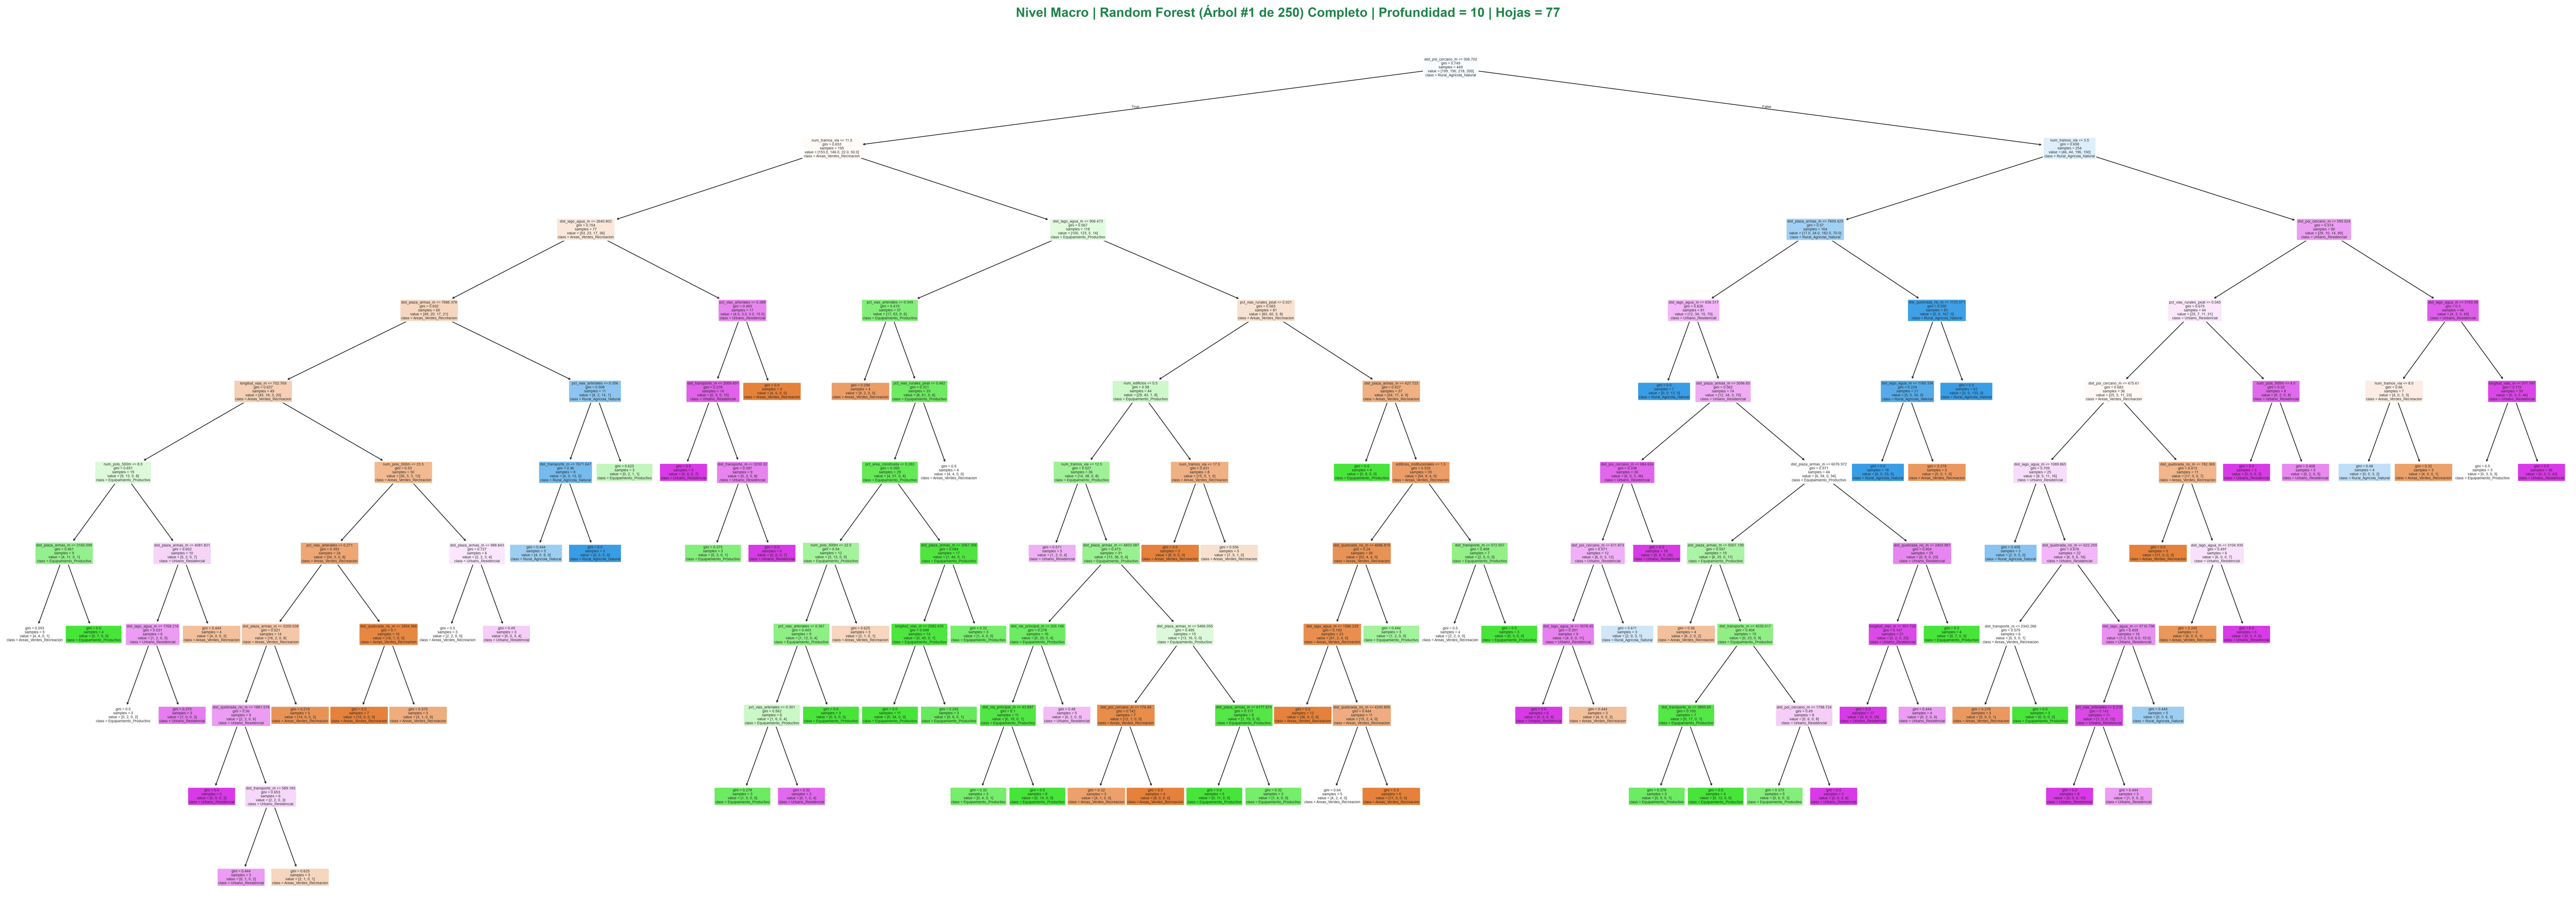
\includegraphics[width=0.99\textwidth]{figures/03_arbol_rf_001_completo.png}
    \caption{Primer árbol completo de \textbf{Random Forest} en el Nivel Macro (Árbol \#1 de $250$, profundidad $= 10$, $77$ hojas terminales).}
    \label{fig:nb03_rf1}
\end{figure}

\begin{figure}[H]
    \centering
    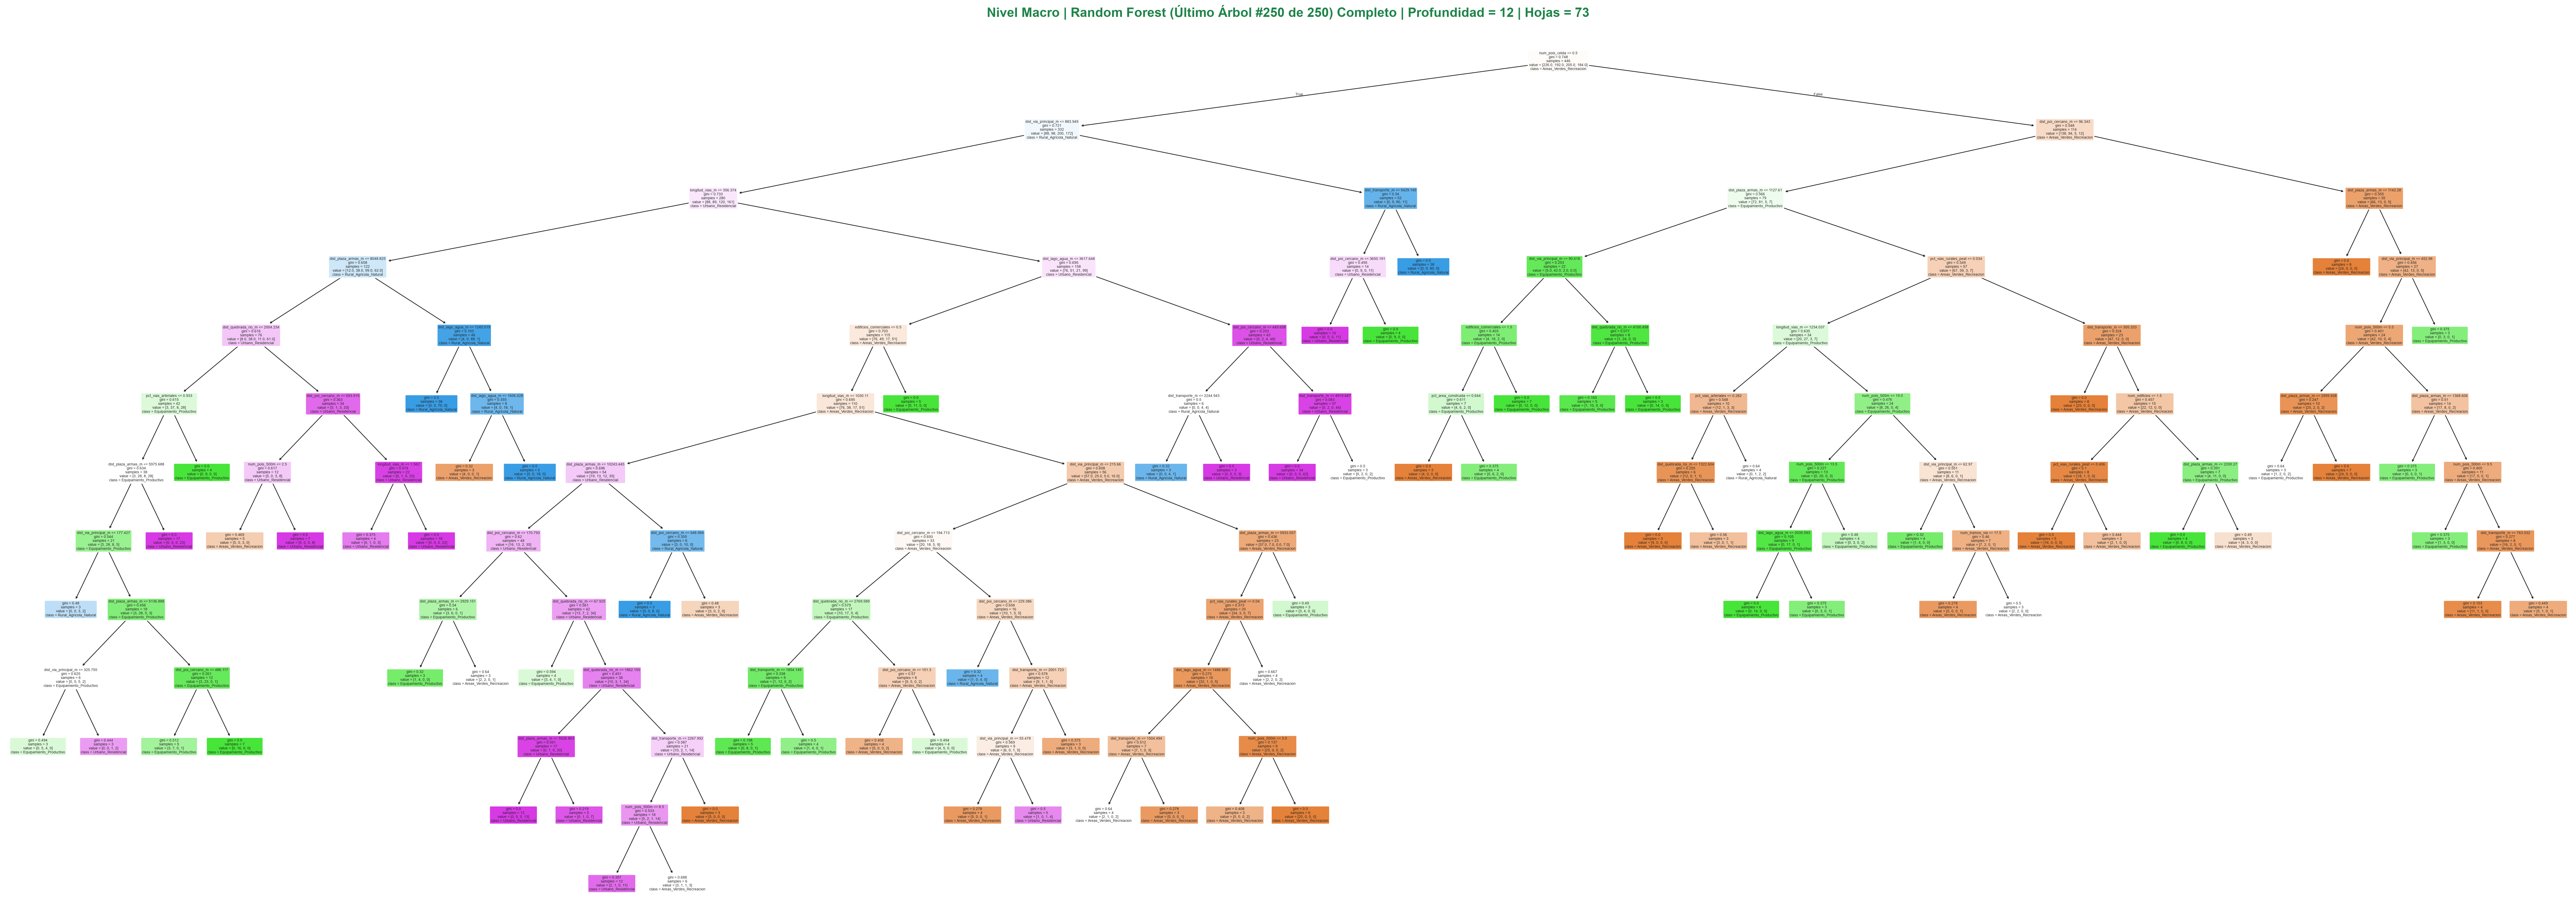
\includegraphics[width=0.99\textwidth]{figures/03_arbol_rf_250_completo.png}
    \caption{Último árbol completo de \textbf{Random Forest} en el Nivel Macro (Árbol \#250 de $250$, profundidad $= 12$, $73$ hojas terminales).}
    \label{fig:nb03_rf250}
\end{figure}

\subsubsection{Modelos 3 y 4 — \texttt{XGBoost} y \texttt{LightGBM}}

\begin{figure}[H]
    \centering
    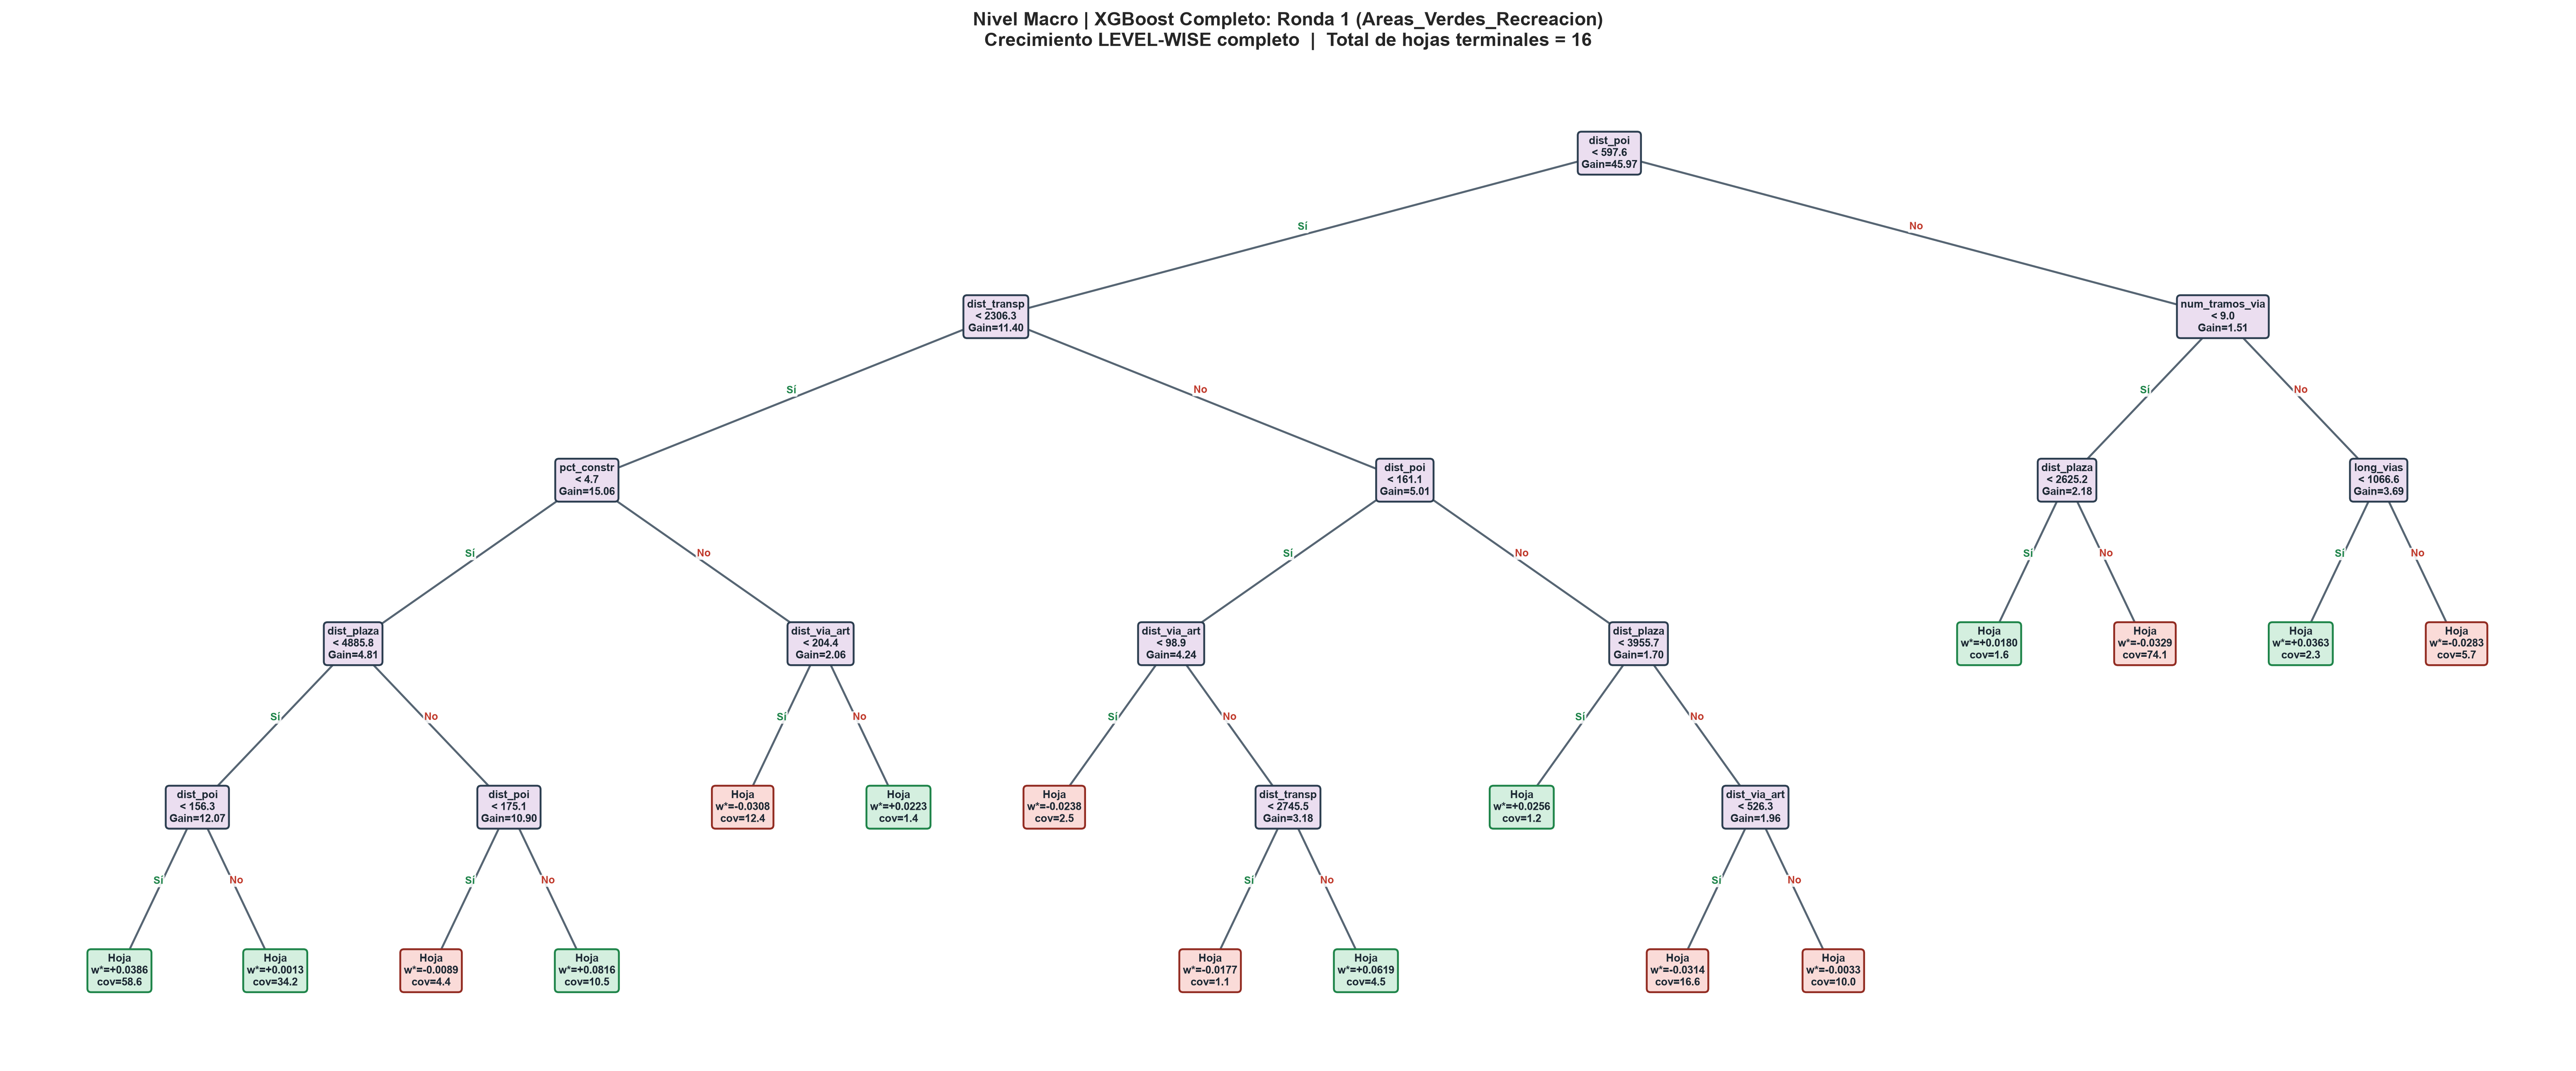
\includegraphics[width=0.99\textwidth]{figures/03_arbol_xgboost_ronda1_completo.png}
    \caption{Árbol completo de \textbf{XGBoost} en la Ronda~1 del Nivel Macro (clase \texttt{Areas\_Verdes\_Recreacion}, $16$ hojas terminales, crecimiento \textit{level-wise}).}
    \label{fig:nb03_xgb1}
\end{figure}

\begin{figure}[H]
    \centering
    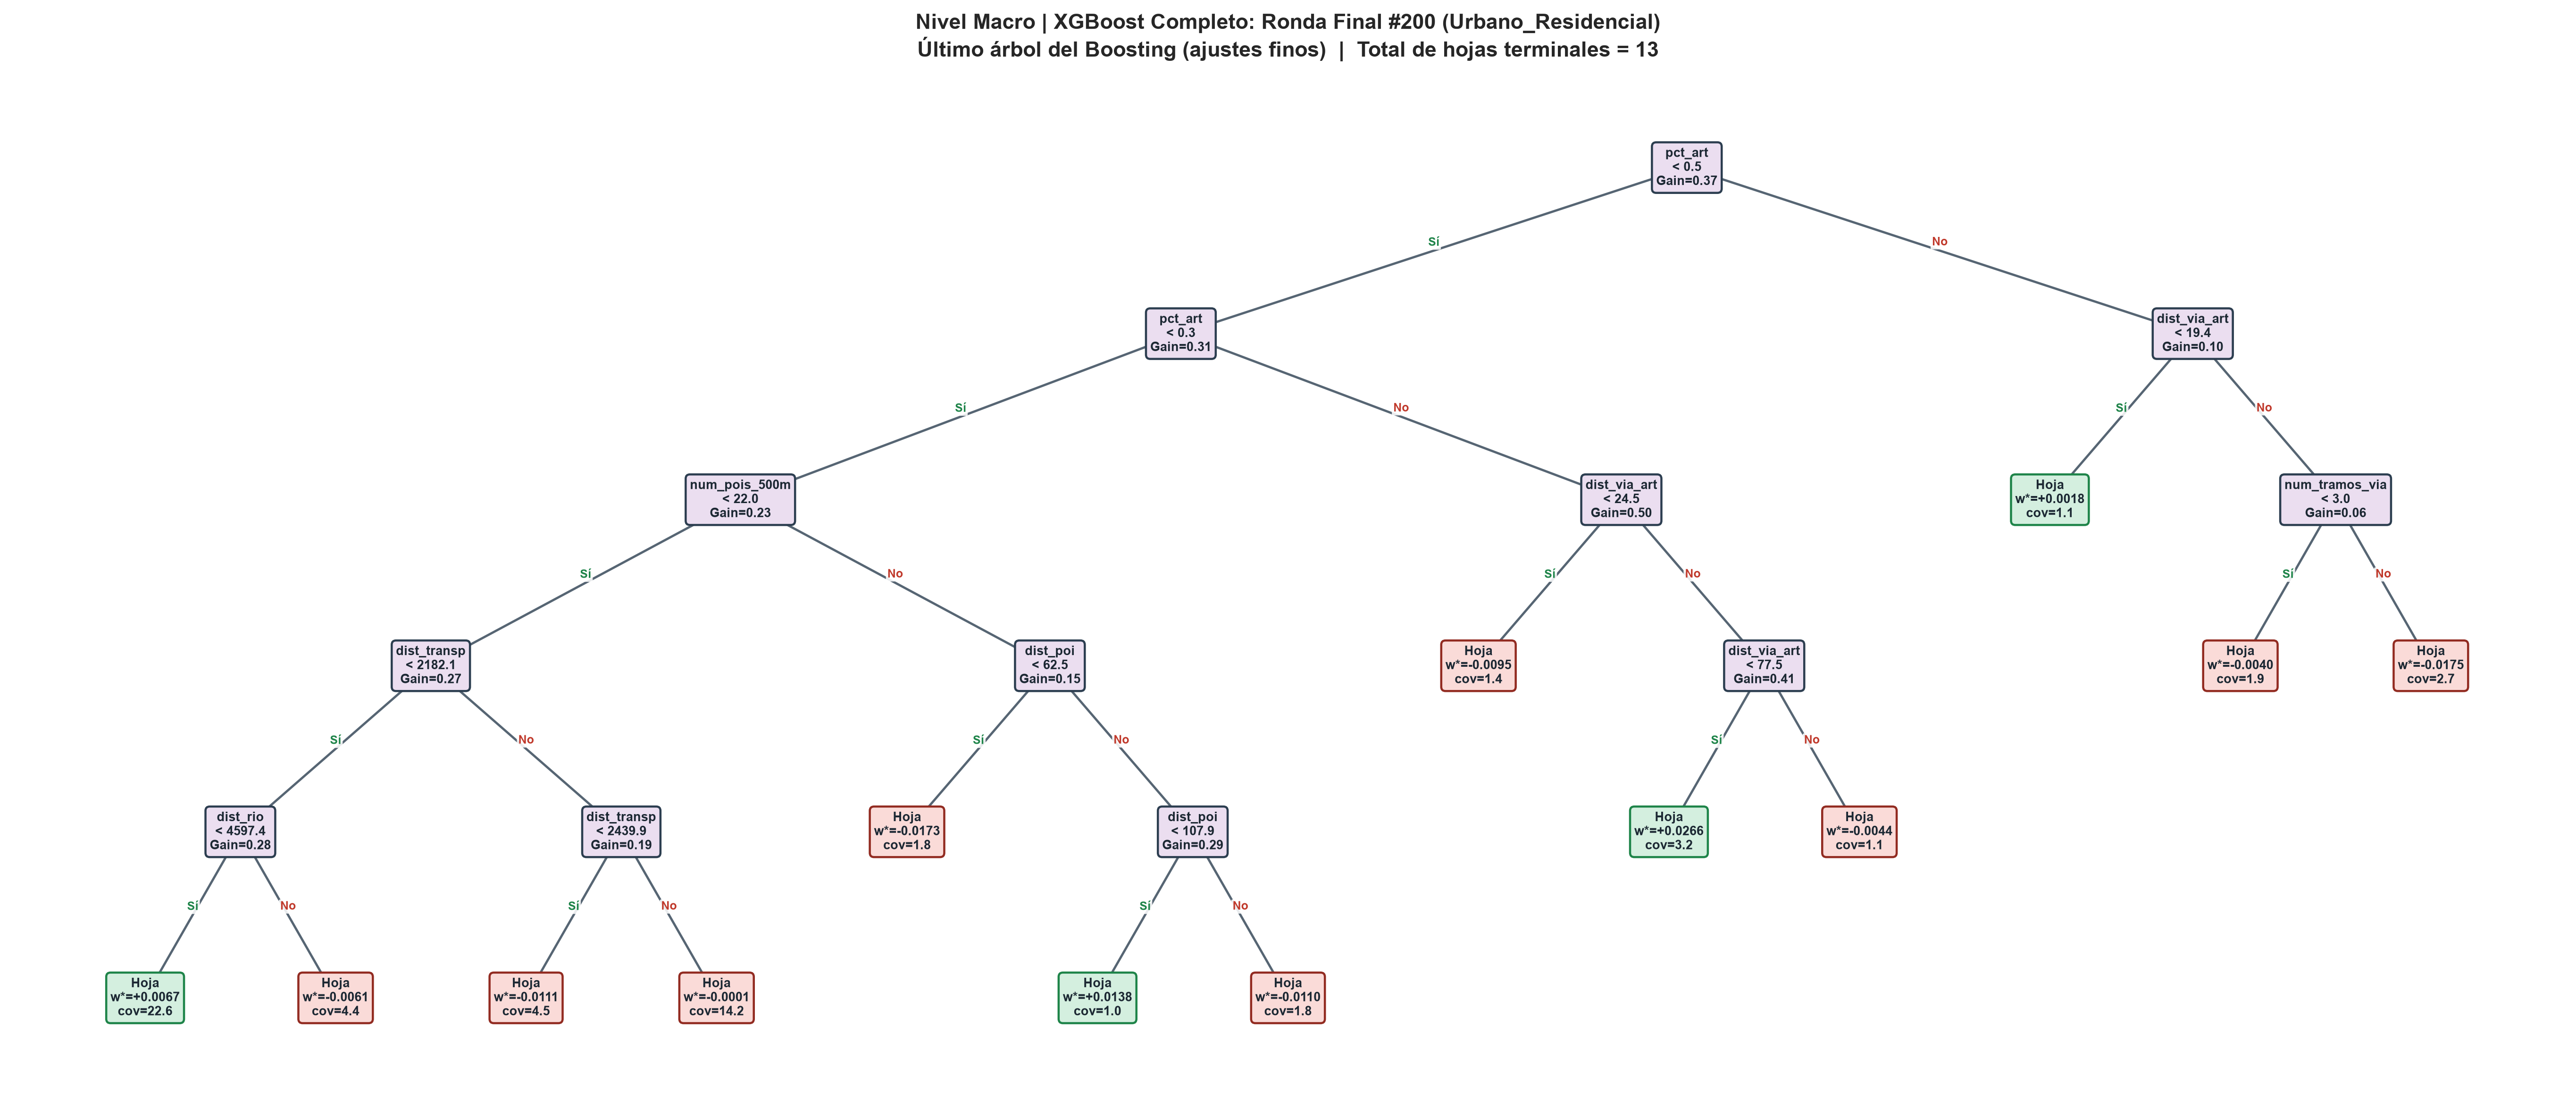
\includegraphics[width=0.96\textwidth]{figures/03_arbol_xgboost_ronda200_completo.png}
    \caption{Árbol completo de \textbf{XGBoost} en la Ronda Final~\#200 (clase \texttt{Urbano\_Residencial}, $13$ hojas terminales).}
    \label{fig:nb03_xgb200}
\end{figure}

\begin{figure}[H]
    \centering
    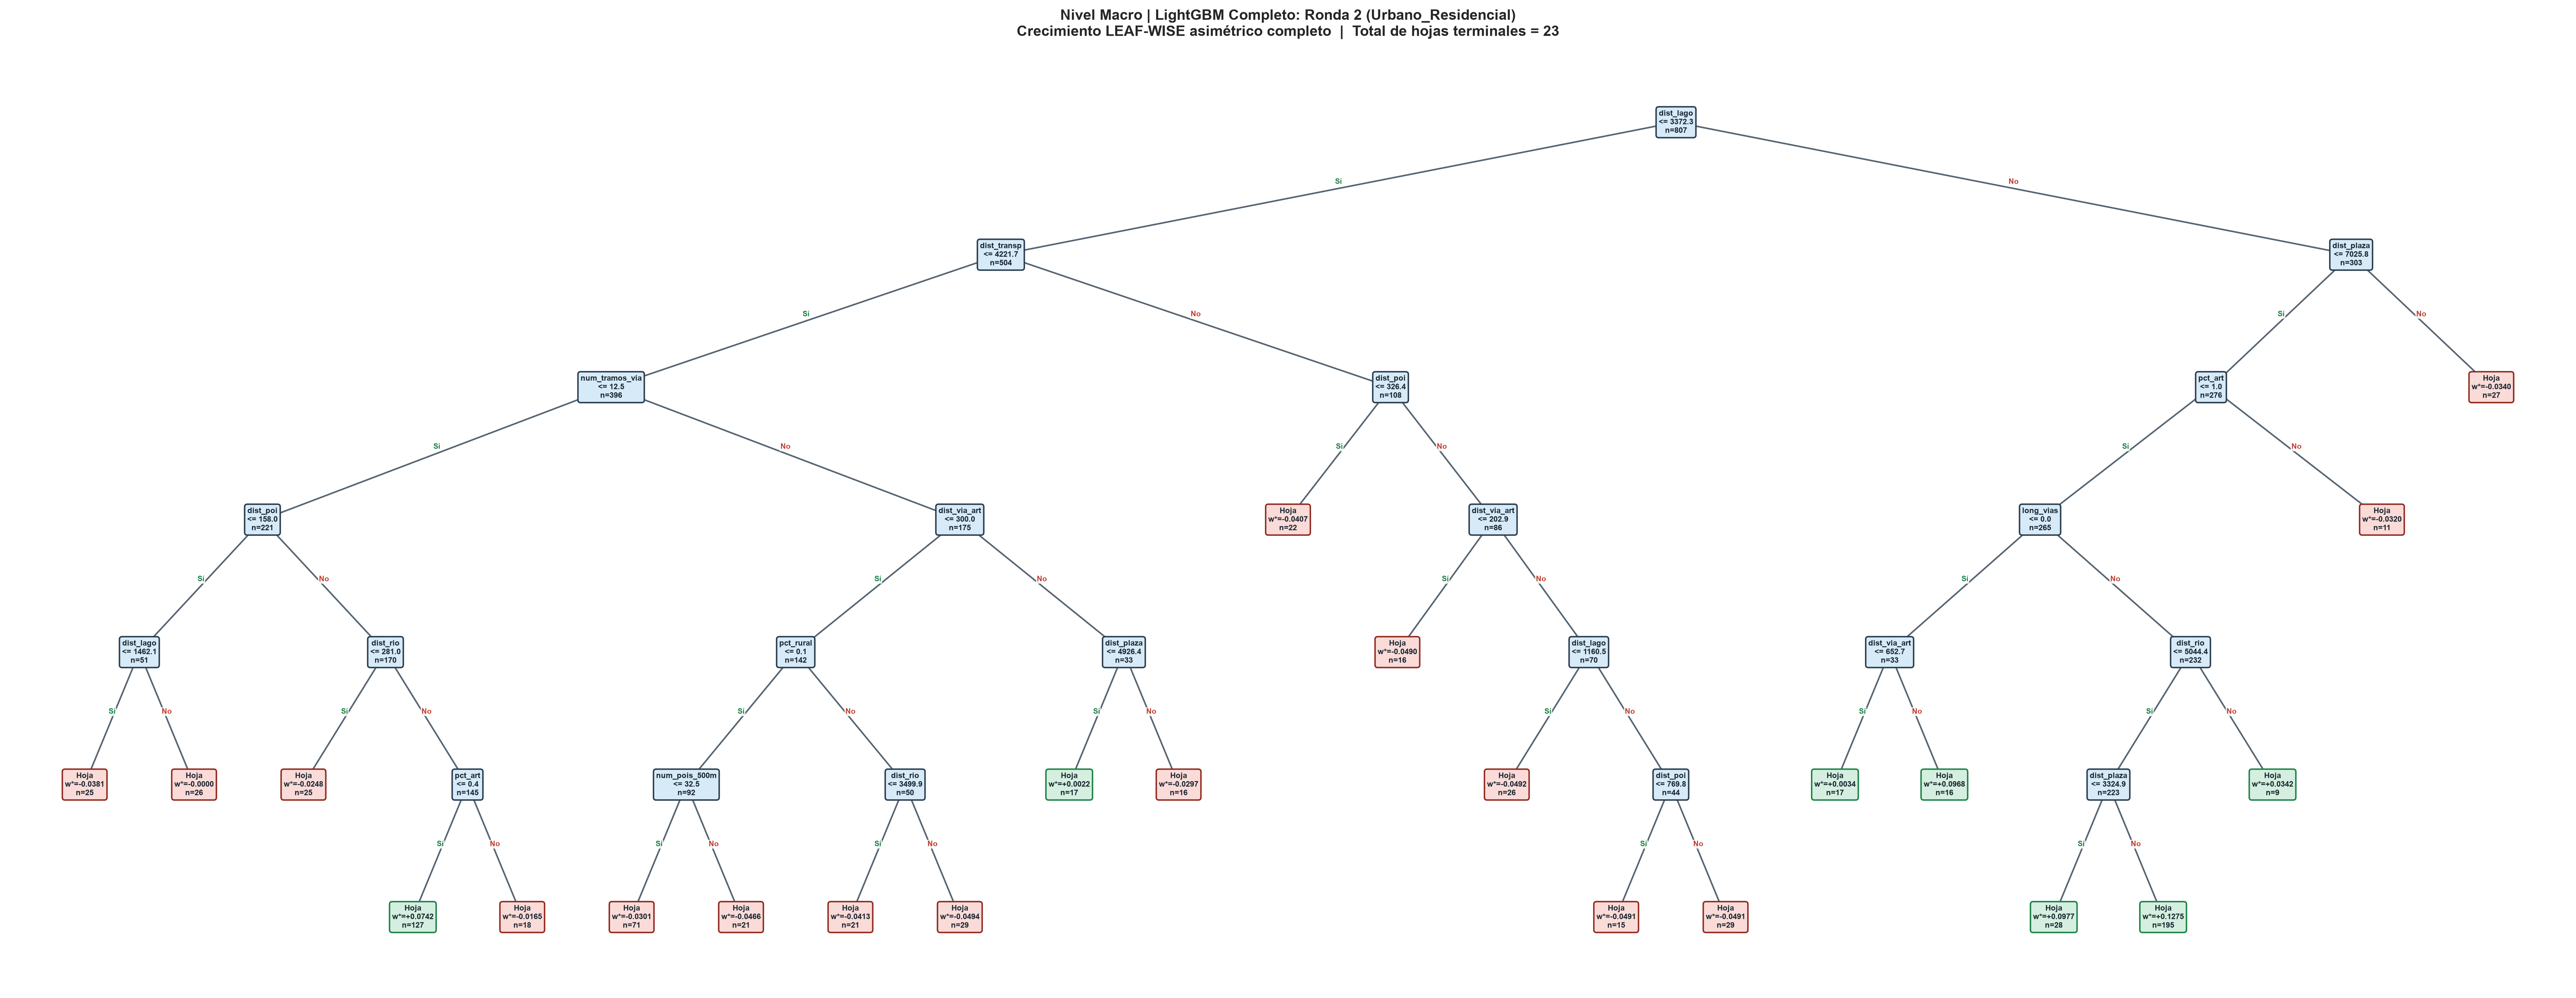
\includegraphics[width=0.99\textwidth]{figures/03_arbol_lightgbm_ronda2_completo.png}
    \caption{Árbol completo de \textbf{LightGBM} en la Ronda~2 del Nivel Macro (clase \texttt{Urbano\_Residencial}, $23$ hojas terminales, crecimiento \textit{leaf-wise}).}
    \label{fig:nb03_lgbm2}
\end{figure}

\begin{figure}[H]
    \centering
    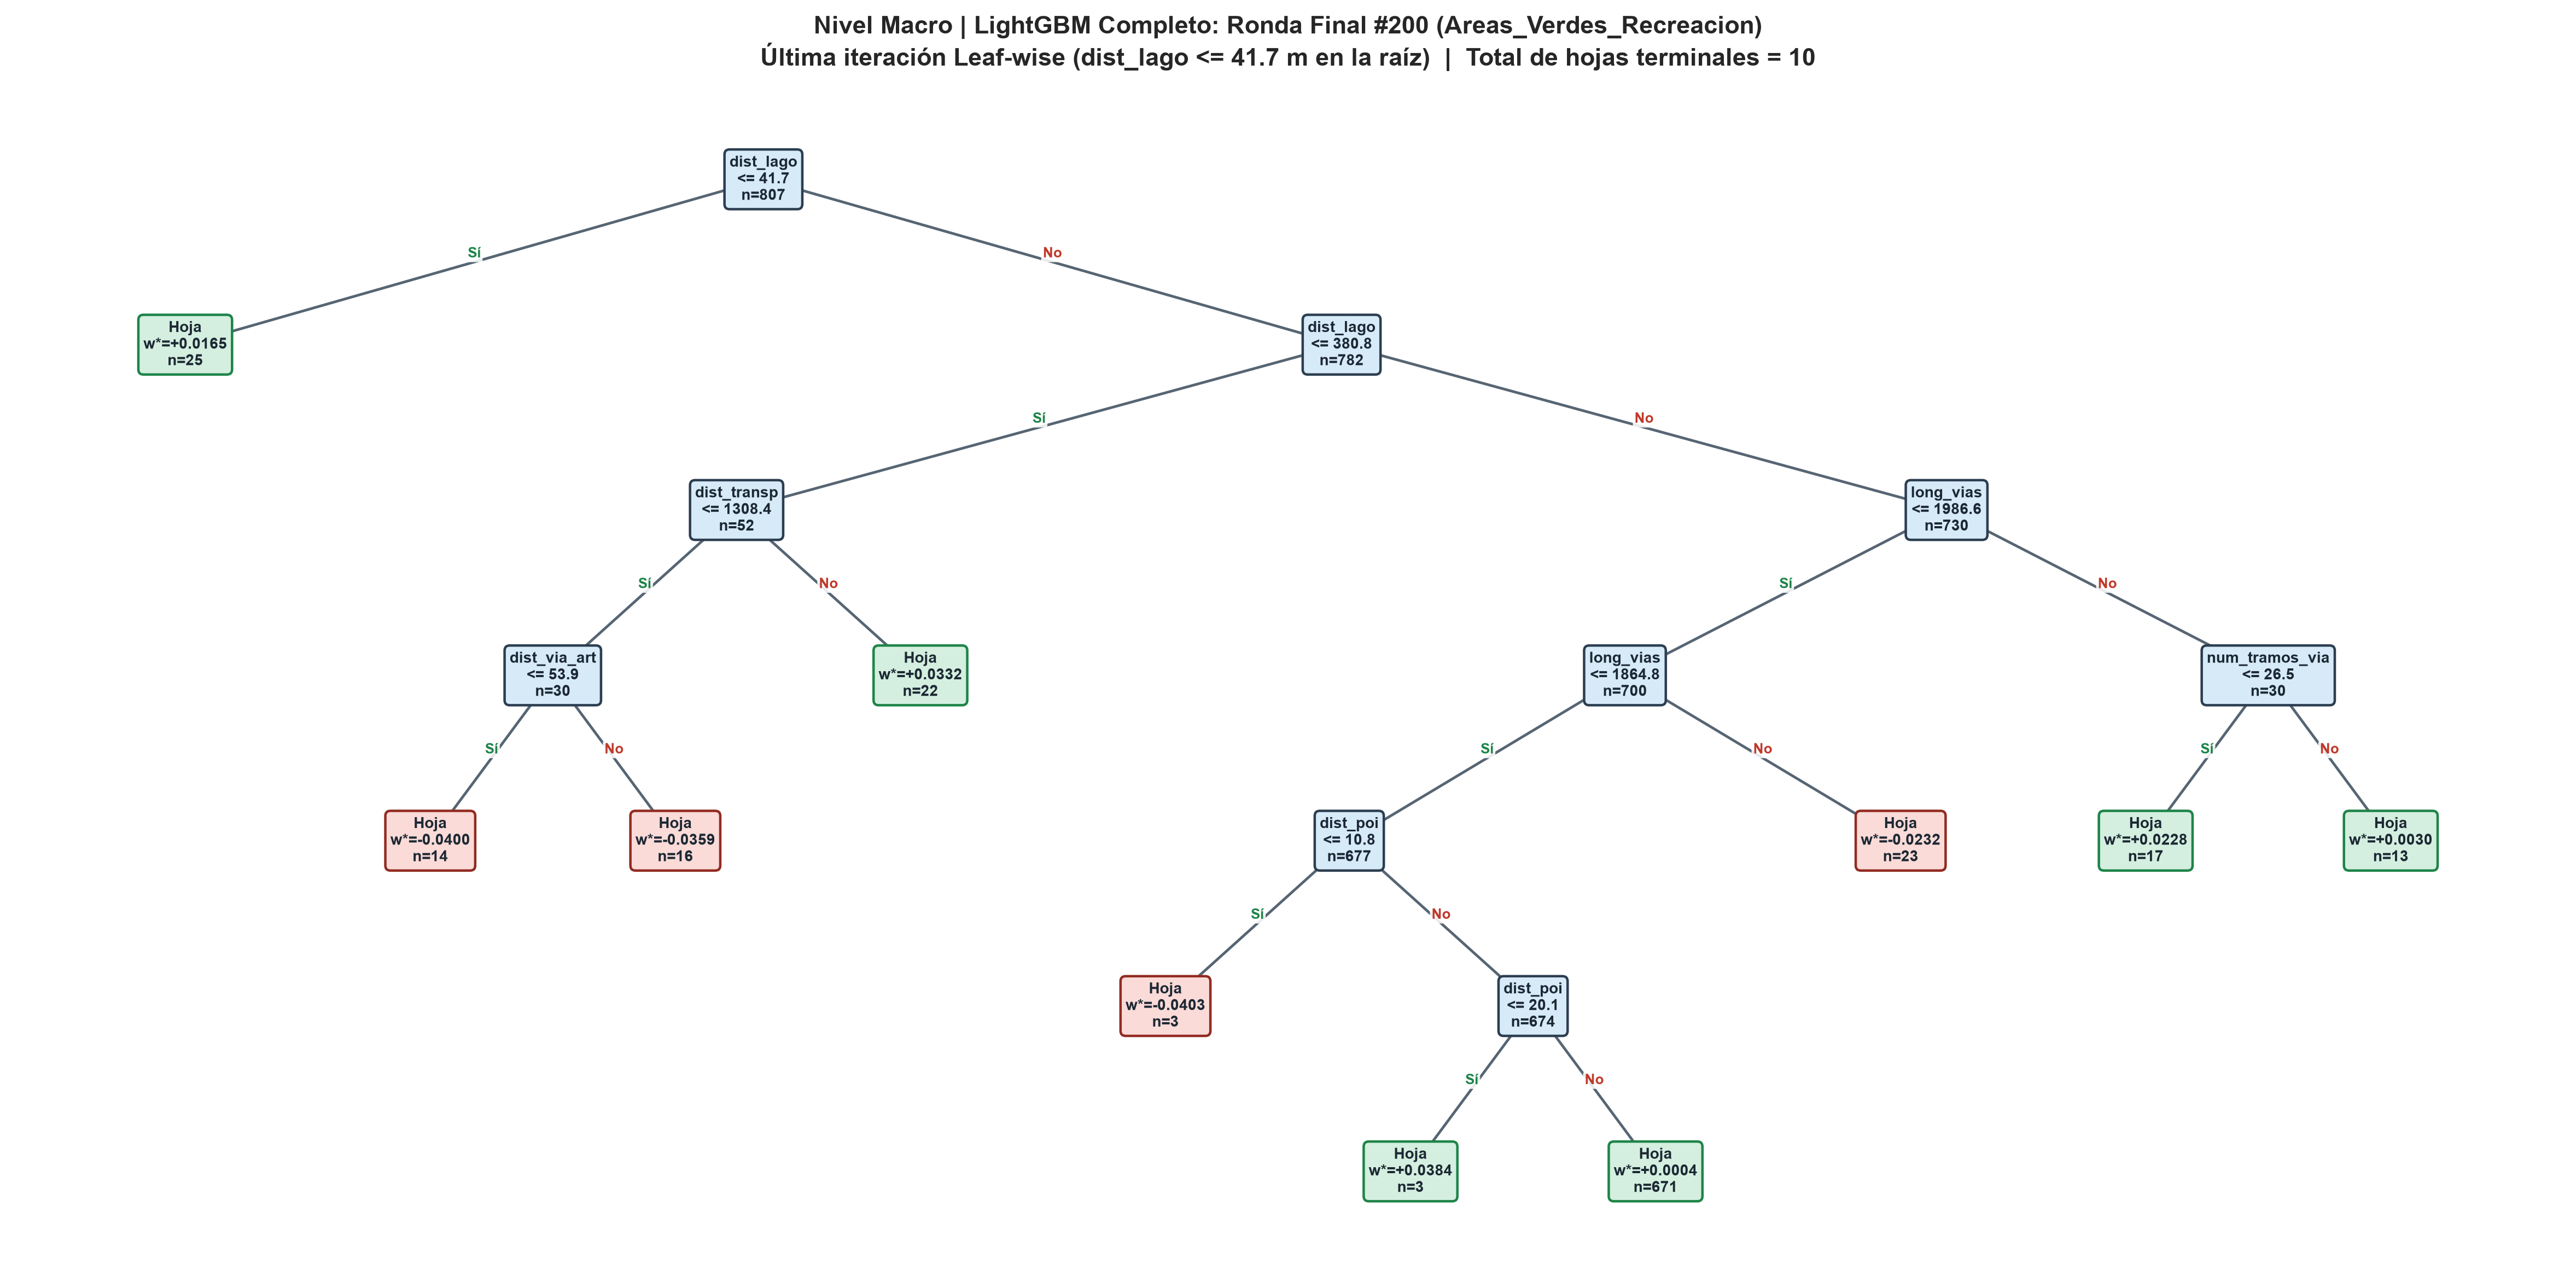
\includegraphics[width=0.95\textwidth]{figures/03_arbol_lightgbm_ronda200_completo.png}
    \caption{Árbol completo de \textbf{LightGBM} en la Ronda Final~\#200 (clase \texttt{Areas\_Verdes\_Recreacion}, $10$ hojas terminales): evidencia la regla geográfica \texttt{dist\_lago <= 41.7 m} en la raíz.}
    \label{fig:nb03_lgbm200}
\end{figure}

\subsection{Matrices de Confusión e Importancia de Variables (\textit{Feature Importance})}

\begin{figure}[H]
    \centering
    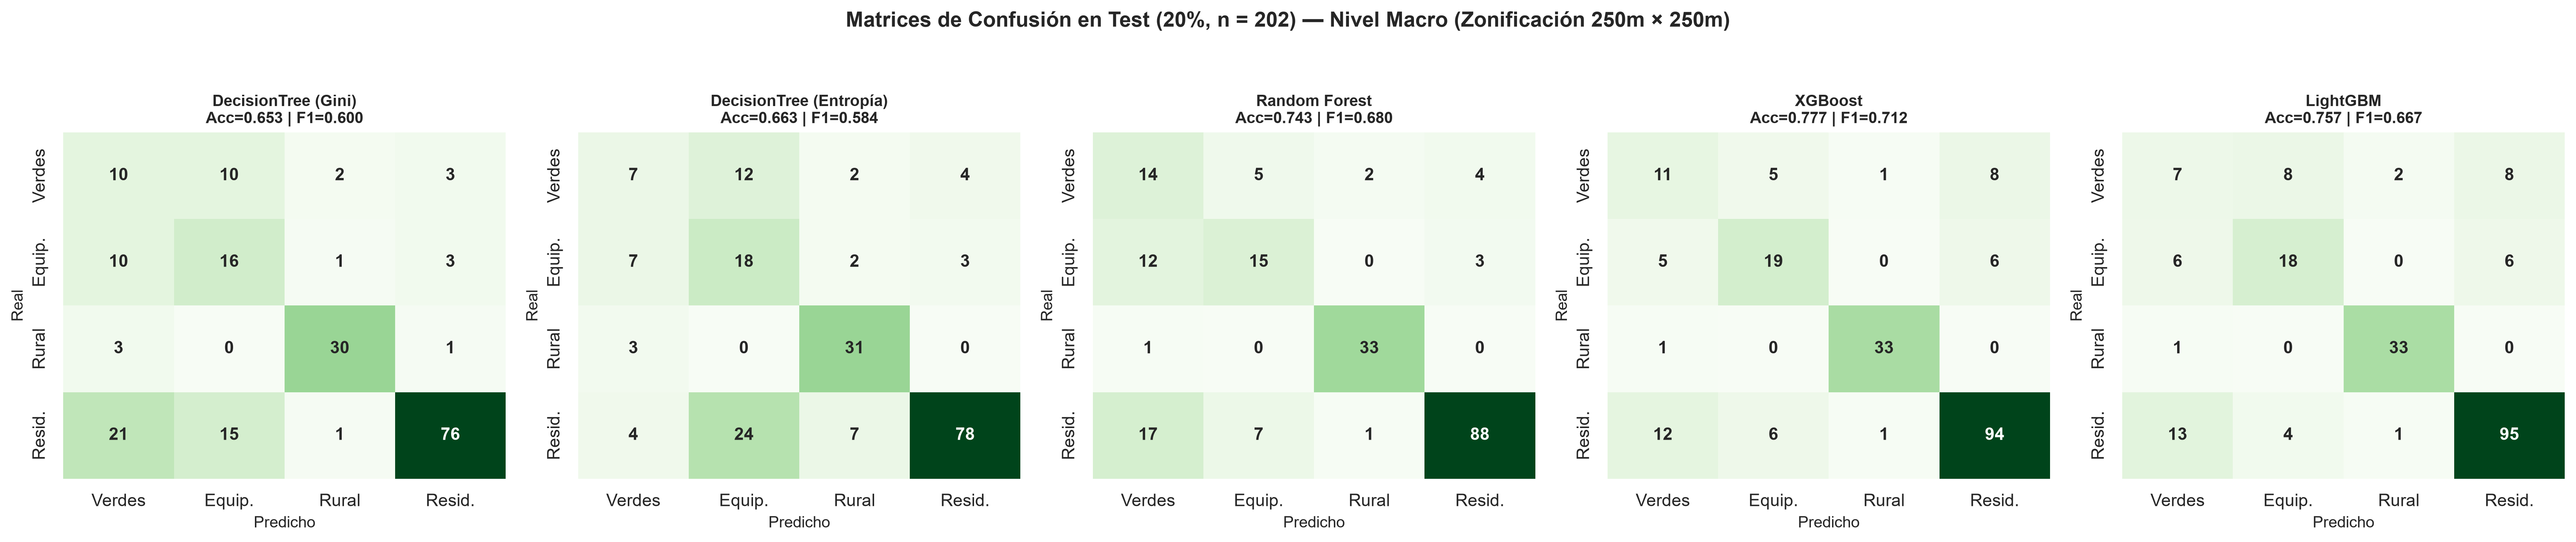
\includegraphics[width=0.99\textwidth]{figures/03_matrices_confusion_macro.png}
    \caption{Matrices de confusión $4 \times 4$ en Test ($20\%$, $n = 202$ celdas) para las cinco configuraciones del Nivel Macro.}
    \label{fig:nb03_cm}
\end{figure}


\begin{figure}[H]
    \centering
    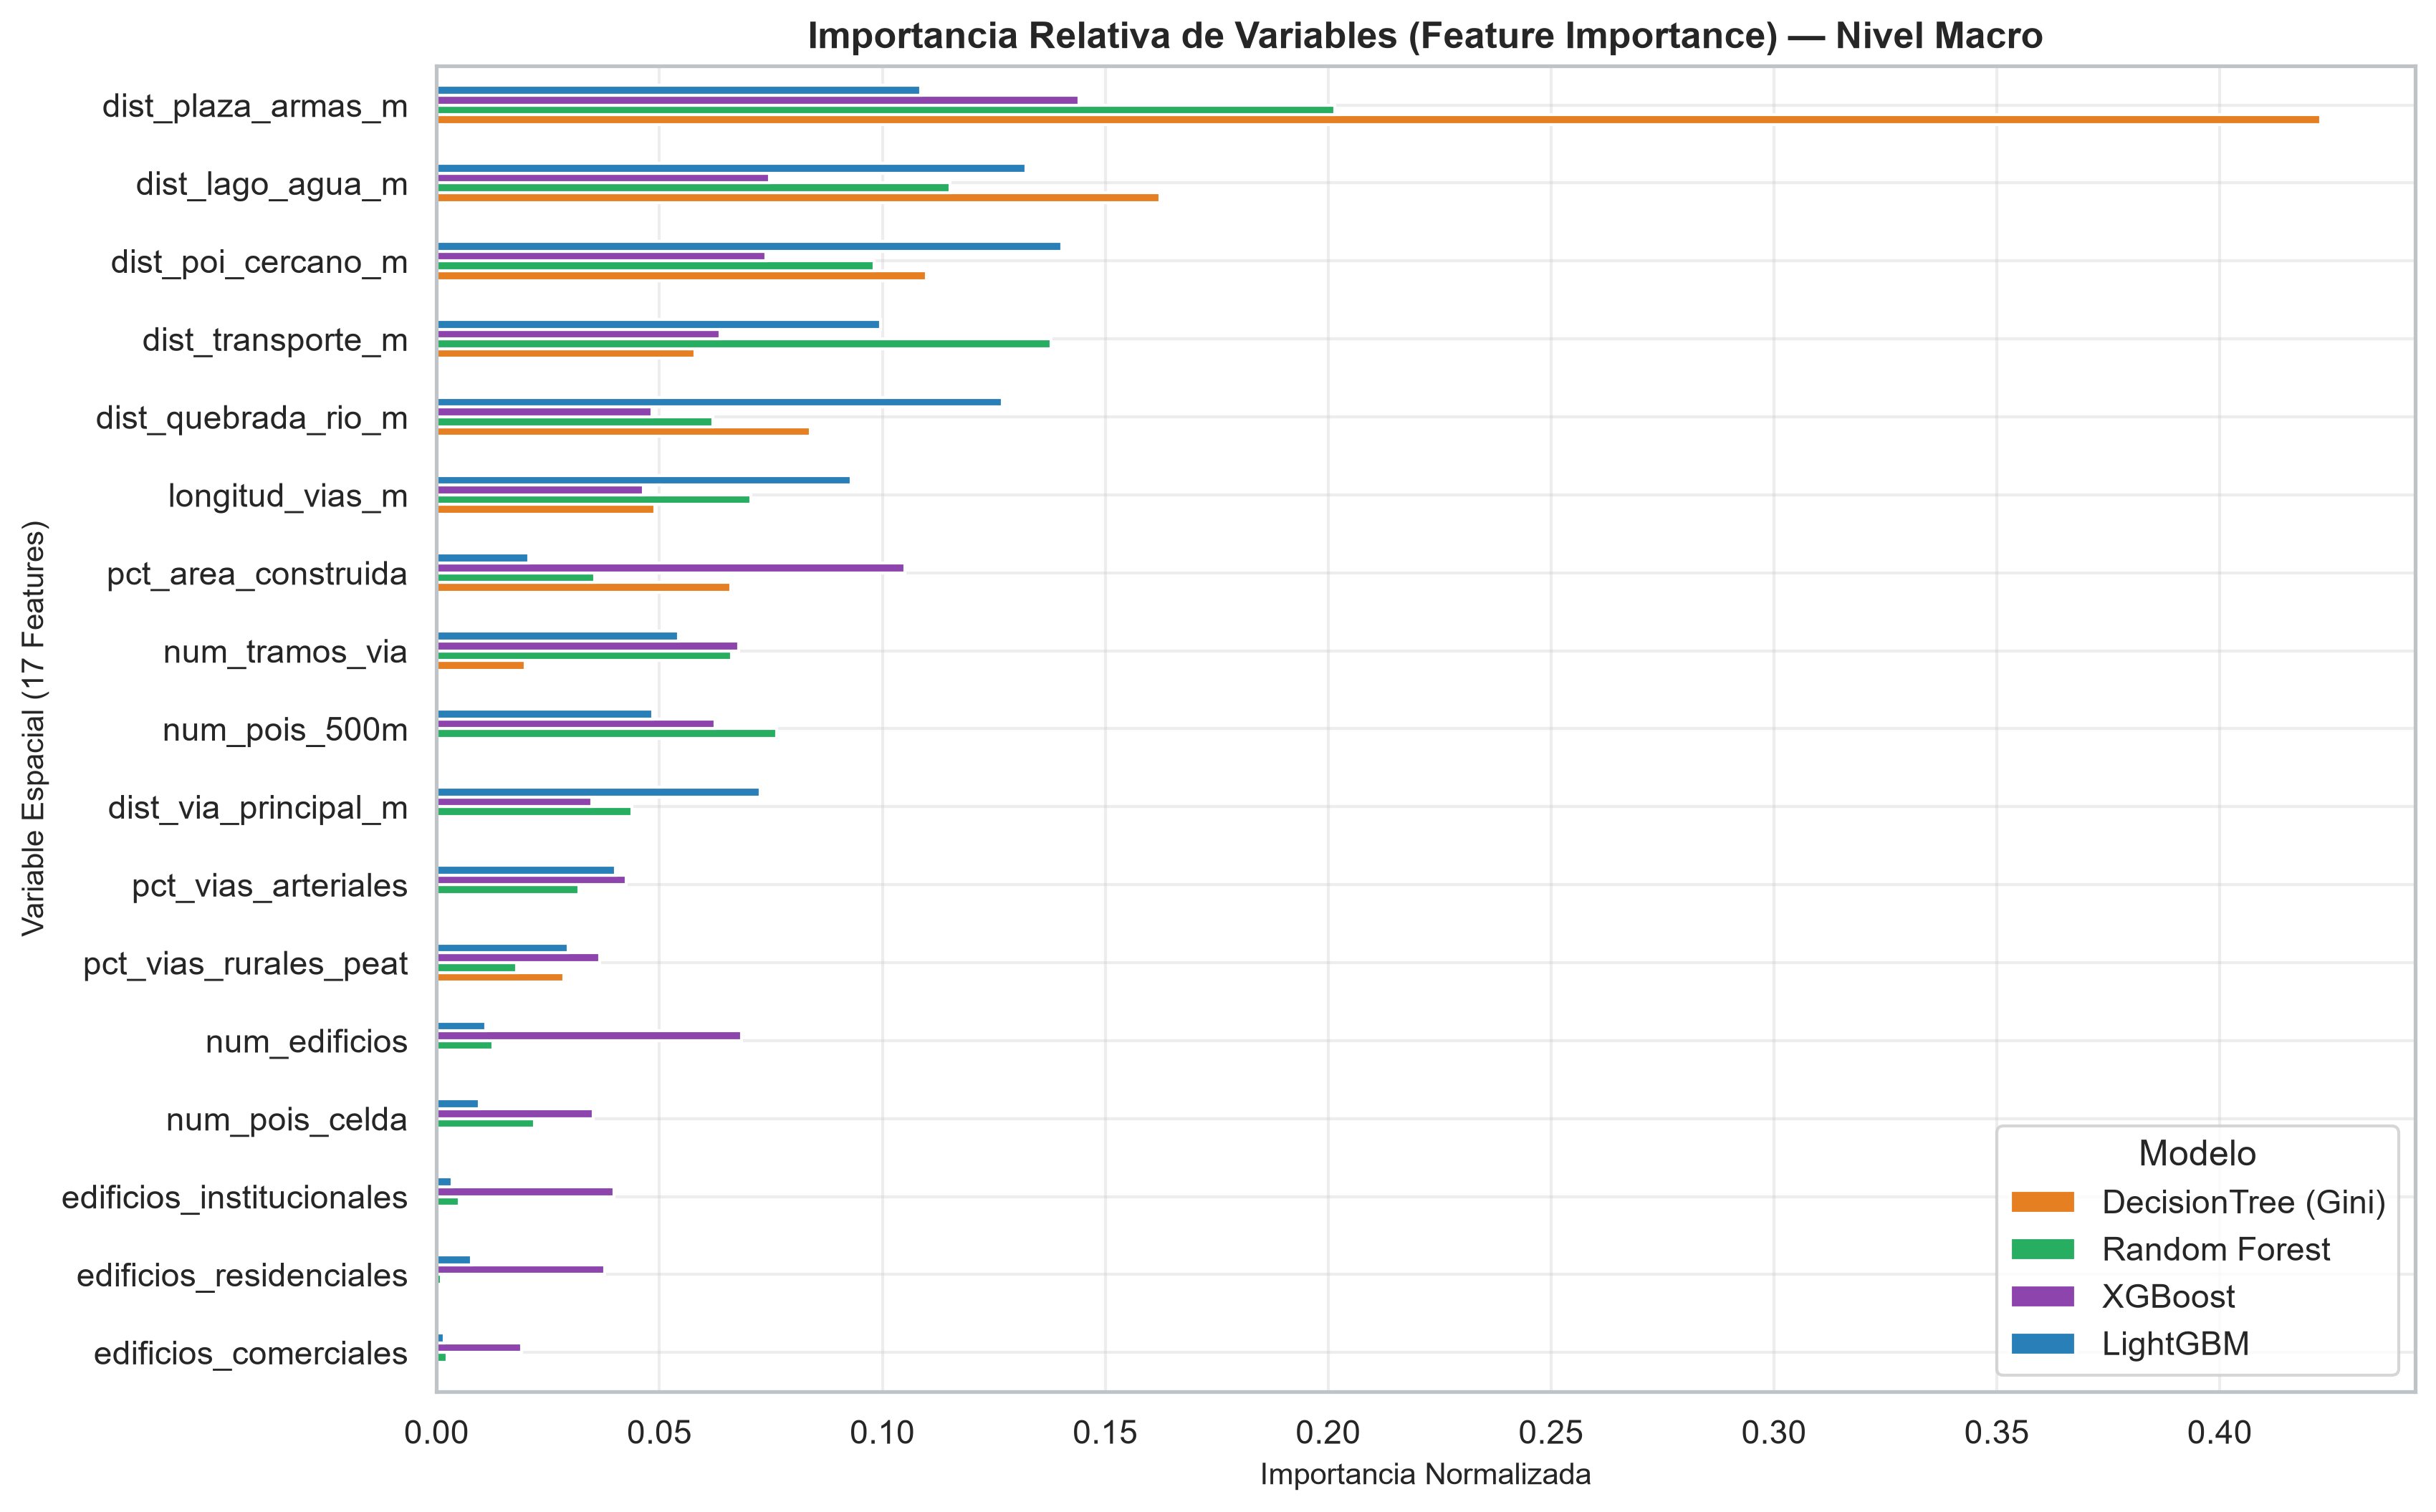
\includegraphics[width=0.88\textwidth]{figures/03_feature_importance_macro.png}
    \caption{Importancia relativa normalizada (\textit{Feature Importance}) de las $17$ variables espaciales en el Nivel Macro.}
    \label{fig:nb03_fi}
\end{figure}

\subsection{Reentrenamiento e Imputación Final}

Siguiendo el mismo protocolo riguroso de reentrenamiento aplicado en el Nivel Micro, una vez elegido el ganador por \texttt{CV-5 F1-Macro} (\textbf{Random Forest}, $0.6980$), se instanció un modelo limpio con exactamente los mismos hiperparámetros y se reentrenó sobre el \textbf{100\% de las $1{,}009$ celdas verificadas}. Posteriormente se predijo la zonificación de las \textbf{$1{,}091$ celdas activas sin etiqueta}, consolidando la capa completa de $2{,}100$ celdas en \texttt{puno\_zonificacion\_macro.geojson} (Tabla~\ref{tab:imputacion_macro}).

\begin{table}[H]
    \centering
    \caption{Distribución final de las $2{,}100$ celdas activas ($250\text{ m} \times 250\text{ m}$) del Distrito de Puno tras la imputación con Random Forest.}
    \label{tab:imputacion_macro}
    \setlength{\tabcolsep}{7pt}
    \small
    \begin{adjustbox}{max width=\textwidth}
    \begin{tabular}{lrrr}
        \toprule
        \rowcolor{verdeHeader}
        \textcolor{white}{\textbf{Zonificación Final (\texttt{zona\_final})}} & \textcolor{white}{\textbf{Verificado (OSM)}} & \textcolor{white}{\textbf{Predicho (ML — RF)}} & \textcolor{white}{\textbf{Total Celdas}} \\
        \midrule
        \texttt{Urbano\_Residencial} & 566 & 404 & \textbf{970} ($46.2\%$) \\
        \rowcolor{verdeSuave!50}
        \texttt{Rural\_Agricola\_Natural} & 167 & 632 & \textbf{799} ($38.0\%$) \\
        \texttt{Equipamiento\_Productivo} & 149 & 45 & \textbf{194} ($9.2\%$) \\
        \rowcolor{verdeSuave!50}
        \texttt{Areas\_Verdes\_Recreacion} & 127 & 10 & \textbf{137} ($6.5\%$) \\
        \midrule
        \rowcolor{verdeSuave}
        \textbf{Total Celdas Activas} & \textbf{1{,}009} ($48.0\%$) & \textbf{1{,}091} ($52.0\%$) & \textbf{2{,}100} ($100.0\%$) \\
        \bottomrule
    \end{tabular}
    \end{adjustbox}
\end{table}

La Figura~\ref{fig:mapa_macro_folium} presenta el mapa interactivo generado en Folium (\texttt{mapa\_macro\_zonificacion.html}) integrando las celdas verificadas y las predichas sobre la geografía de Puno.

\begin{figure}[H]
    \centering
    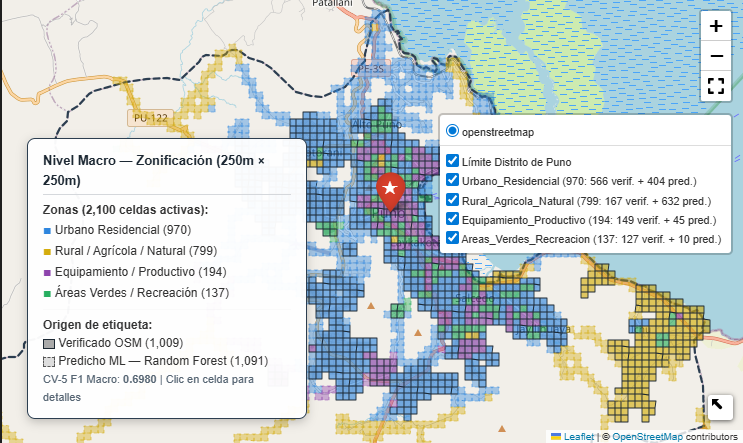
\includegraphics[width=0.96\textwidth]{figures/Nivel_Macro_Mapa.png}
    \caption{Mapa interactivo del Nivel Macro (\texttt{mapa\_macro\_zonificacion.html}) mostrando la zonificación de las $2{,}100$ celdas de $250\text{ m} \times 250\text{ m}$, diferenciando las $1{,}009$ celdas verificadas en OSM (borde sólido oscuro) de las $1{,}091$ predichas por Random Forest (borde punteado).}
    \label{fig:mapa_macro_folium}
\end{figure}

% ==============================================================================
% SECCIÓN 5: EVALUACIÓN COMPARATIVA GLOBAL Y SÍNTESIS MULTIESCALA (BASADO EN NB 04)
% ==============================================================================
\section{Evaluación Comparativa Global y Síntesis Multiescala}
\label{sec:comparativa}

Una vez completados los modelados independientes a Nivel Micro y Nivel Macro, esta sección consolida la evidencia empírica en una evaluación transversal de los cuatro paradigmas de aprendizaje basados en árboles, contrastando rendimiento predictivo, eficiencia computacional, sensibilidad al criterio de impureza (Gini vs. Entropía), grado de acuerdo entre algoritmos y coherencia territorial al superponer las dos escalas urbanas.

\subsection{Comparativa Global de Modelos: Nivel Micro vs. Nivel Macro}

La Tabla~\ref{tab:comparativa_global} reúne el desempeño consolidado de las cinco configuraciones evaluadas en ambas escalas territoriales, mientras que la Tabla~\ref{tab:detallada_global} desglosa las métricas en el conjunto de prueba diferenciando los promedios \textit{Macro} y (ponderado por soporte).

\begin{table}[H]
    \centering
    \caption{Tabla comparativa global de rendimiento y tiempo de entrenamiento en Nivel Micro ($n_{\text{test}}=37$) y Nivel Macro ($n_{\text{test}}=202$).}
    \label{tab:comparativa_global}
    \setlength{\tabcolsep}{4pt}
    \footnotesize
    \begin{adjustbox}{max width=\textwidth}
    \begin{tabular}{lllrrrrr}
        \toprule
        \rowcolor{verdeHeader}
        \textcolor{white}{\textbf{Escala}} & \textcolor{white}{\textbf{Modelo}} & \textcolor{white}{\textbf{Paradigma}} & \textcolor{white}{\textbf{Test Acc}} & \textcolor{white}{\textbf{Test F1(M)}} & \textcolor{white}{\textbf{CV-5 Acc}} & \textcolor{white}{\textbf{CV-5 F1(M)}} & \textcolor{white}{\textbf{Tiempo (ms)}} \\
        \midrule
        \rowcolor{azulSuave!65}
        Micro & \textbf{LightGBM} (Ganador CV) & Leaf-wise Boosting & 0.8108 & 0.7874 & \textbf{0.7667} & \textbf{0.7496} & 63.35 \\
        Micro & \textbf{Random Forest} (Mejor Test) & Ensamble Bagging & \textbf{0.8378} & \textbf{0.8115} & 0.7664 & 0.7465 & 408.88 \\
        Micro & XGBoost & Gradient Boosting & 0.7838 & 0.7545 & 0.7395 & 0.7160 & 254.47 \\
        Micro & DecisionTree (Entropía) & Árbol Simple & 0.6757 & 0.6204 & 0.7009 & 0.6744 & 1.87 \\
        Micro & DecisionTree (Gini) & Árbol Simple & 0.8108 & 0.7831 & 0.6793 & 0.6517 & \textbf{1.76} \\
        \midrule
        \rowcolor{azulSuave!65}
        Macro & \textbf{Random Forest} (Ganador CV) & Ensamble Bagging & 0.7426 & 0.6803 & 0.7681 & \textbf{0.6980} & 475.37 \\
        Macro & \textbf{XGBoost} (Mejor Test) & Gradient Boosting & \textbf{0.7772} & \textbf{0.7120} & \textbf{0.7760} & 0.6977 & 733.07 \\
        Macro & LightGBM & Leaf-wise Boosting & 0.7574 & 0.6670 & 0.7691 & 0.6767 & 310.12 \\
        Macro & DecisionTree (Gini) & Árbol Simple & 0.6535 & 0.5996 & 0.6809 & 0.6318 & \textbf{5.20} \\
        Macro & DecisionTree (Entropía) & Árbol Simple & 0.6634 & 0.5841 & 0.6671 & 0.5999 & 7.92 \\
        \bottomrule
    \end{tabular}
    \end{adjustbox}
\end{table}

\begin{table}[H]
    \centering
    \caption{Desglose completo de métricas en Test (\textit{Accuracy}, \textit{Balanced Accuracy}, \textit{Macro} y \textit{Weighted}) en ambas escalas.}
    \label{tab:detallada_global}
    \setlength{\tabcolsep}{4pt}
    \footnotesize
    \begin{adjustbox}{max width=\textwidth}
    \begin{tabular}{llrrrrrrr}
        \toprule
        \rowcolor{verdeHeader}
        \textcolor{white}{\textbf{Escala}} & \textcolor{white}{\textbf{Modelo}} & \textcolor{white}{\textbf{Acc.}} & \textcolor{white}{\textbf{Bal. Acc}} & \textcolor{white}{\textbf{Prec(M)}} & \textcolor{white}{\textbf{Prec(W)}} & \textcolor{white}{\textbf{Rec(M)}} & \textcolor{white}{\textbf{F1(M)}} & \textcolor{white}{\textbf{F1(W)}} \\
        \midrule
        Micro & DecisionTree (Gini) & 0.8108 & 0.8000 & 0.8125 & 0.8318 & 0.8000 & 0.7831 & 0.7999 \\
        \rowcolor{verdeSuave!50}
        Micro & DecisionTree (Entropía) & 0.6757 & 0.6500 & 0.6347 & 0.6684 & 0.6500 & 0.6204 & 0.6518 \\
        Micro & \textbf{Random Forest} & \textbf{0.8378} & \textbf{0.8333} & \textbf{0.8681} & \textbf{0.8846} & \textbf{0.8333} & \textbf{0.8115} & \textbf{0.8248} \\
        \rowcolor{verdeSuave!50}
        Micro & XGBoost & 0.7838 & 0.7667 & 0.7676 & 0.7896 & 0.7667 & 0.7545 & 0.7749 \\
        Micro & LightGBM & 0.8108 & 0.7889 & 0.7879 & 0.8133 & 0.7889 & 0.7874 & 0.8112 \\
        \midrule
        \rowcolor{verdeSuave!50}
        Macro & DecisionTree (Gini) & 0.6535 & 0.6221 & 0.6039 & 0.7468 & 0.6221 & 0.5996 & 0.6851 \\
        Macro & DecisionTree (Entropía) & 0.6634 & 0.6205 & 0.5806 & 0.7283 & 0.6205 & 0.5841 & 0.6794 \\
        \rowcolor{verdeSuave!50}
        Macro & Random Forest & 0.7426 & 0.7023 & 0.6792 & \textbf{0.7944} & 0.7023 & 0.6803 & 0.7604 \\
        Macro & \textbf{XGBoost} & \textbf{0.7772} & \textbf{0.7189} & \textbf{0.7065} & 0.7866 & \textbf{0.7189} & \textbf{0.7120} & \textbf{0.7814} \\
        \rowcolor{verdeSuave!50}
        Macro & LightGBM & 0.7574 & 0.6728 & 0.6619 & 0.7630 & 0.6728 & 0.6670 & 0.7599 \\
        \bottomrule
    \end{tabular}
    \end{adjustbox}
\end{table}

\begin{figure}[H]
    \centering
    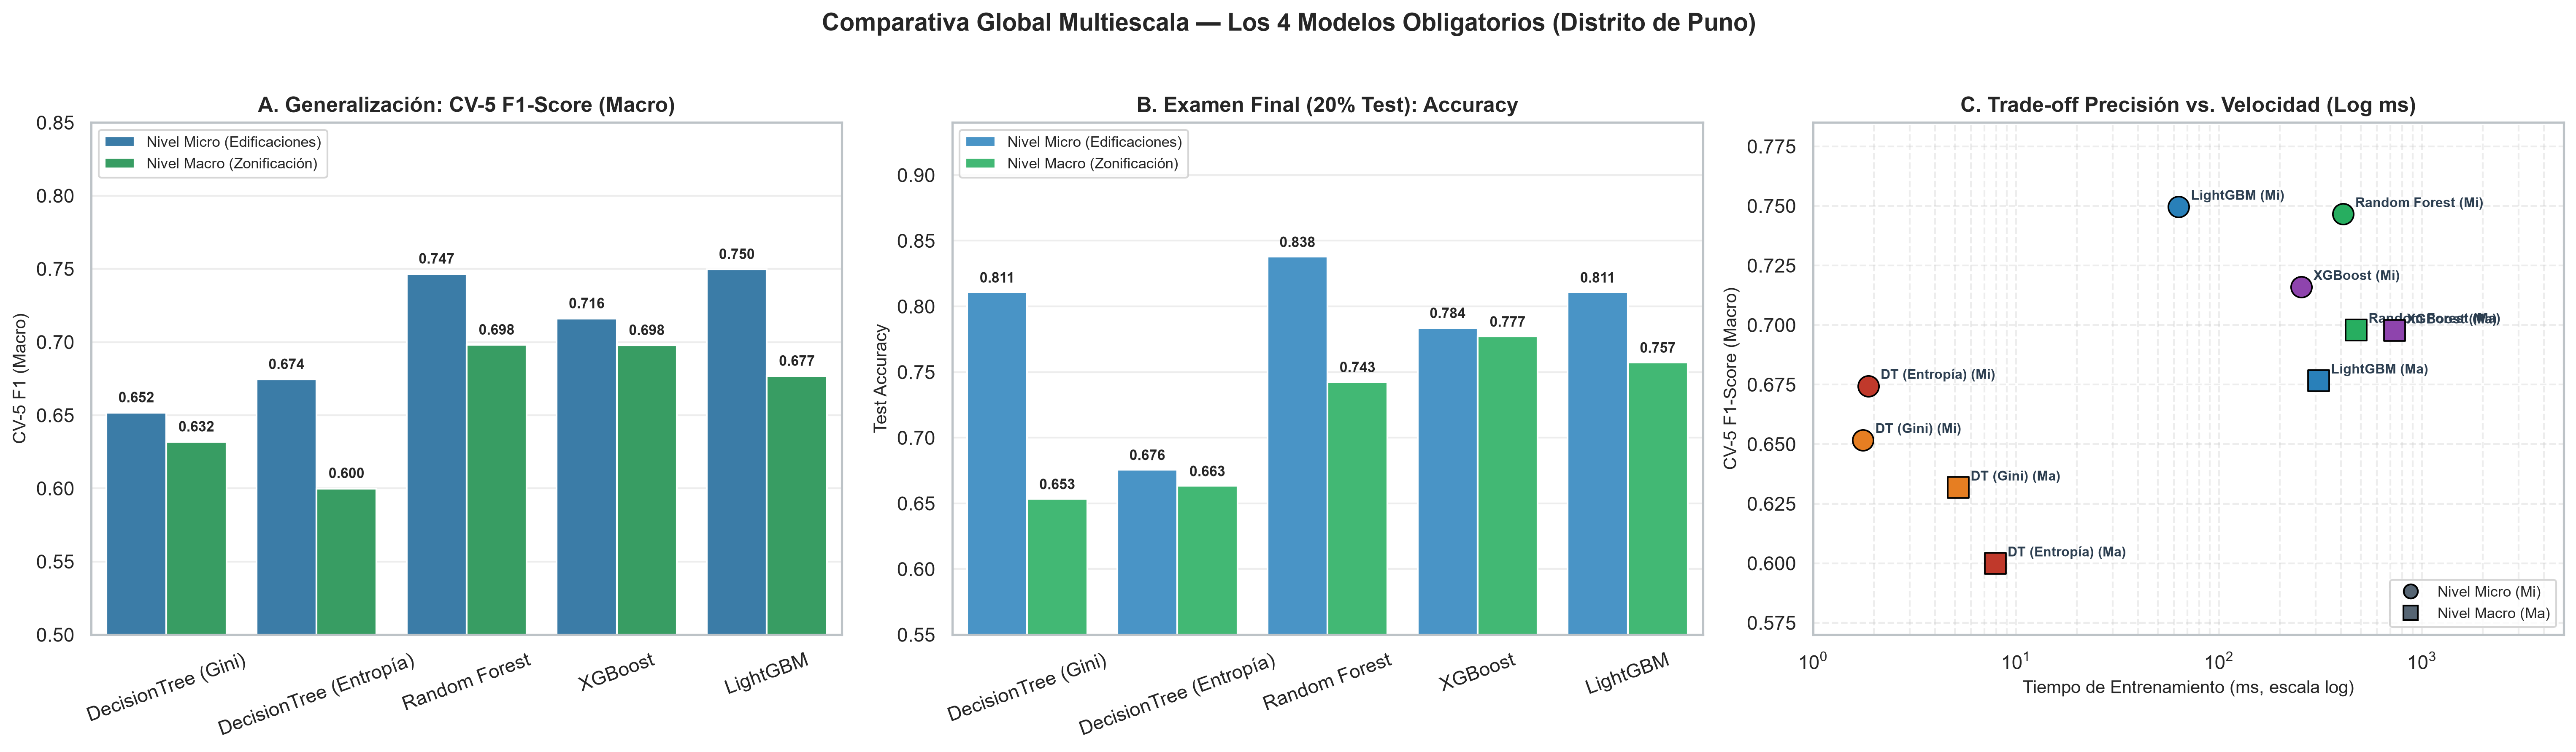
\includegraphics[width=0.98\textwidth]{figures/04_comparativa_global_modelos.png}
    \caption{Comparativa global de los cuatro paradigmas en Nivel Micro y Nivel Macro: validación cruzada (Panel A), conjunto de prueba independiente (Panel B) y frontera de compromiso entre rendimiento y tiempo de entrenamiento en escala logarítmica (Panel C).}
    \label{fig:nb04_global}
\end{figure}

\begin{table}[H]
    \centering
    \caption{Distribución de consenso y discrepancias entre los cuatro paradigmas sobre los conjuntos de prueba independientes.}
    \label{tab:consenso_test}
    \setlength{\tabcolsep}{7pt}
    \small
    \begin{adjustbox}{max width=\textwidth}
    \begin{tabular}{lrrrr}
        \toprule
        \rowcolor{verdeHeader}
        \textcolor{white}{\textbf{Estado de Evaluación en Test}} & \textcolor{white}{\textbf{Micro ($n=37$)}} & \textcolor{white}{\textbf{Micro ($\%$)}} & \textcolor{white}{\textbf{Macro ($n=202$)}} & \textcolor{white}{\textbf{Macro ($\%$)}} \\
        \midrule
        Acierto Unánime ($4/4$ modelos aciertan) & \textbf{27} & \textbf{73.0\%} & \textbf{115} & \textbf{56.9\%} \\
        \rowcolor{verdeSuave!50}
        Discrepancia entre Modelos ($1/4$ a $3/4$) & 8 & 21.6\% & 59 & 29.2\% \\
        Error Unánime ($0/4$ modelos aciertan) & 2 & 5.4\% & 28 & 13.9\% \\
        \midrule
        \rowcolor{verdeSuave}
        \textbf{Total Observaciones en Test} & \textbf{37} & \textbf{100.0\%} & \textbf{202} & \textbf{100.0\%} \\
        \bottomrule
    \end{tabular}
    \end{adjustbox}
\end{table}

\begin{figure}[H]
    \centering
    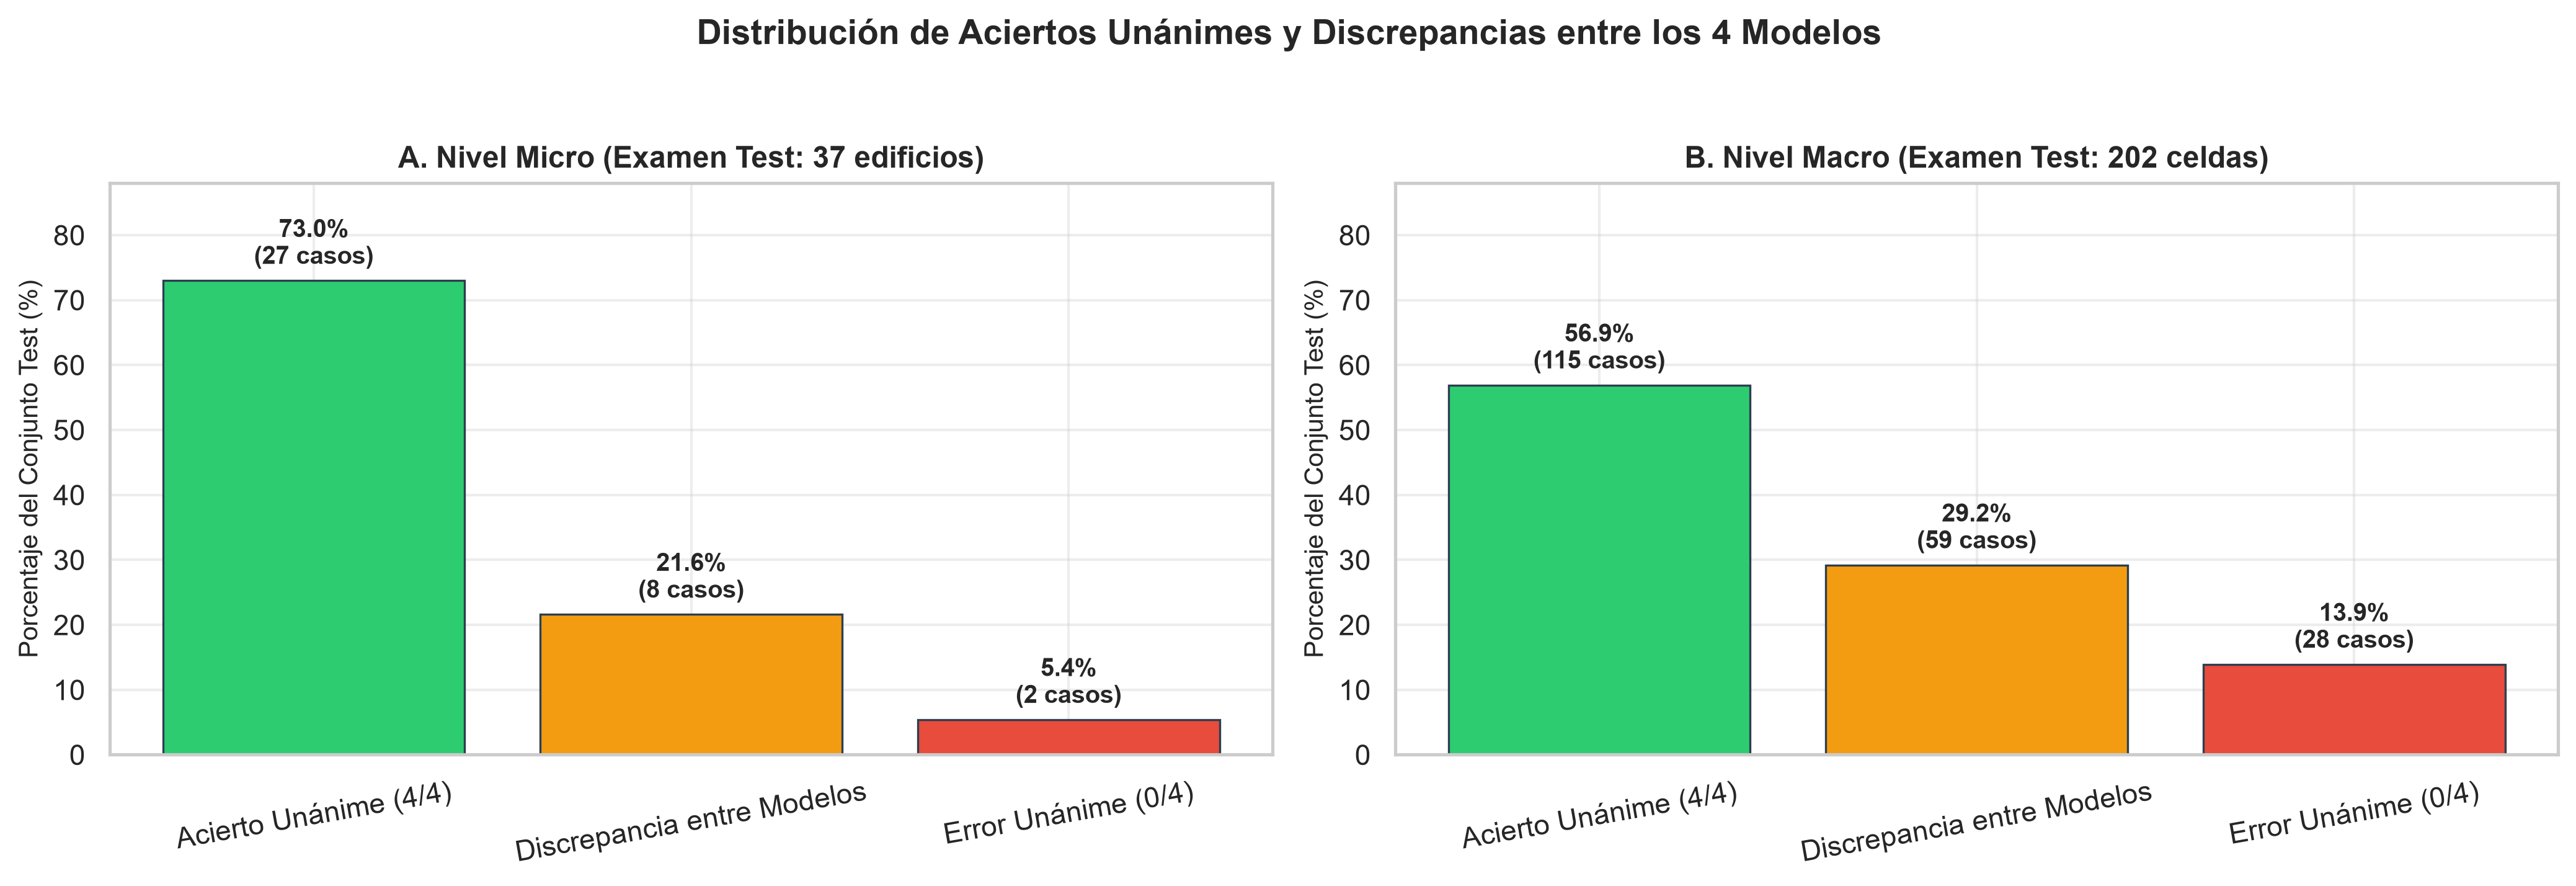
\includegraphics[width=0.96\textwidth]{figures/04_aciertos_discrepancias_test.png}
    \caption{Proporción de aciertos unánimes ($4/4$), discrepancias parciales y errores unánimes ($0/4$) entre los cuatro modelos en Test (Micro y Macro).}
    \label{fig:nb04_discrepancias}
\end{figure}

\subsection{Coherencia Territorial Multiescala y Cartografía Final Integrada}

Para validar si las predicciones independientes de ambos niveles producen una lectura geográfica consistente de la ciudad de Puno, se efectuó una intersección espacial cruzando las $652$ edificaciones clasificadas en el Nivel Micro con las $2{,}100$ celdas zonificadas en el Nivel Macro ($652/652$ edificios emparejados). La Tabla~\ref{tab:coherencia_multiescala} y la Figura~\ref{fig:nb04_coherencia} sintetizan esta matriz de coherencia territorial.

\begin{table}[H]
    \centering
    \caption{Matriz de coherencia territorial multiescala: distribución de las $652$ edificaciones clasificadas (Nivel Micro) dentro de las zonas finales (Nivel Macro).}
    \label{tab:coherencia_multiescala}
    \setlength{\tabcolsep}{6pt}
    \small
    \begin{adjustbox}{max width=\textwidth}
    \begin{tabular}{lrrrr}
        \toprule
        \rowcolor{verdeHeader}
        \textcolor{white}{\textbf{Zona Macro (\texttt{zona\_final})}} & \textcolor{white}{\textbf{Comercial / Serv.}} & \textcolor{white}{\textbf{Institucional}} & \textcolor{white}{\textbf{Residencial}} & \textcolor{white}{\textbf{Total Edif.}} \\
        \midrule
        \texttt{Equipamiento\_Productivo} & 133 ($30.0\%$) & \textbf{189} ($42.6\%$) & 122 ($27.5\%$) & \textbf{444} ($68.1\%$) \\
        \rowcolor{verdeSuave!50}
        \texttt{Areas\_Verdes\_Recreacion} & 38 ($27.1\%$) & \textbf{73} ($52.1\%$) & 29 ($20.7\%$) & \textbf{140} ($21.5\%$) \\
        \texttt{Urbano\_Residencial} & 21 ($48.8\%$) & 17 ($39.5\%$) & 5 ($11.6\%$) & \textbf{43} ($6.6\%$) \\
        \rowcolor{verdeSuave!50}
        \texttt{Rural\_Agricola\_Natural} & 3 ($12.0\%$) & 8 ($32.0\%$) & \textbf{14} ($56.0\%$) & \textbf{25} ($3.8\%$) \\
        \midrule
        \rowcolor{verdeSuave}
        \textbf{Total Edificaciones Micro} & \textbf{195} ($29.9\%$) & \textbf{287} ($44.0\%$) & \textbf{170} ($26.1\%$) & \textbf{652} ($100.0\%$) \\
        \bottomrule
    \end{tabular}
    \end{adjustbox}
\end{table}

\begin{figure}[H]
    \centering
    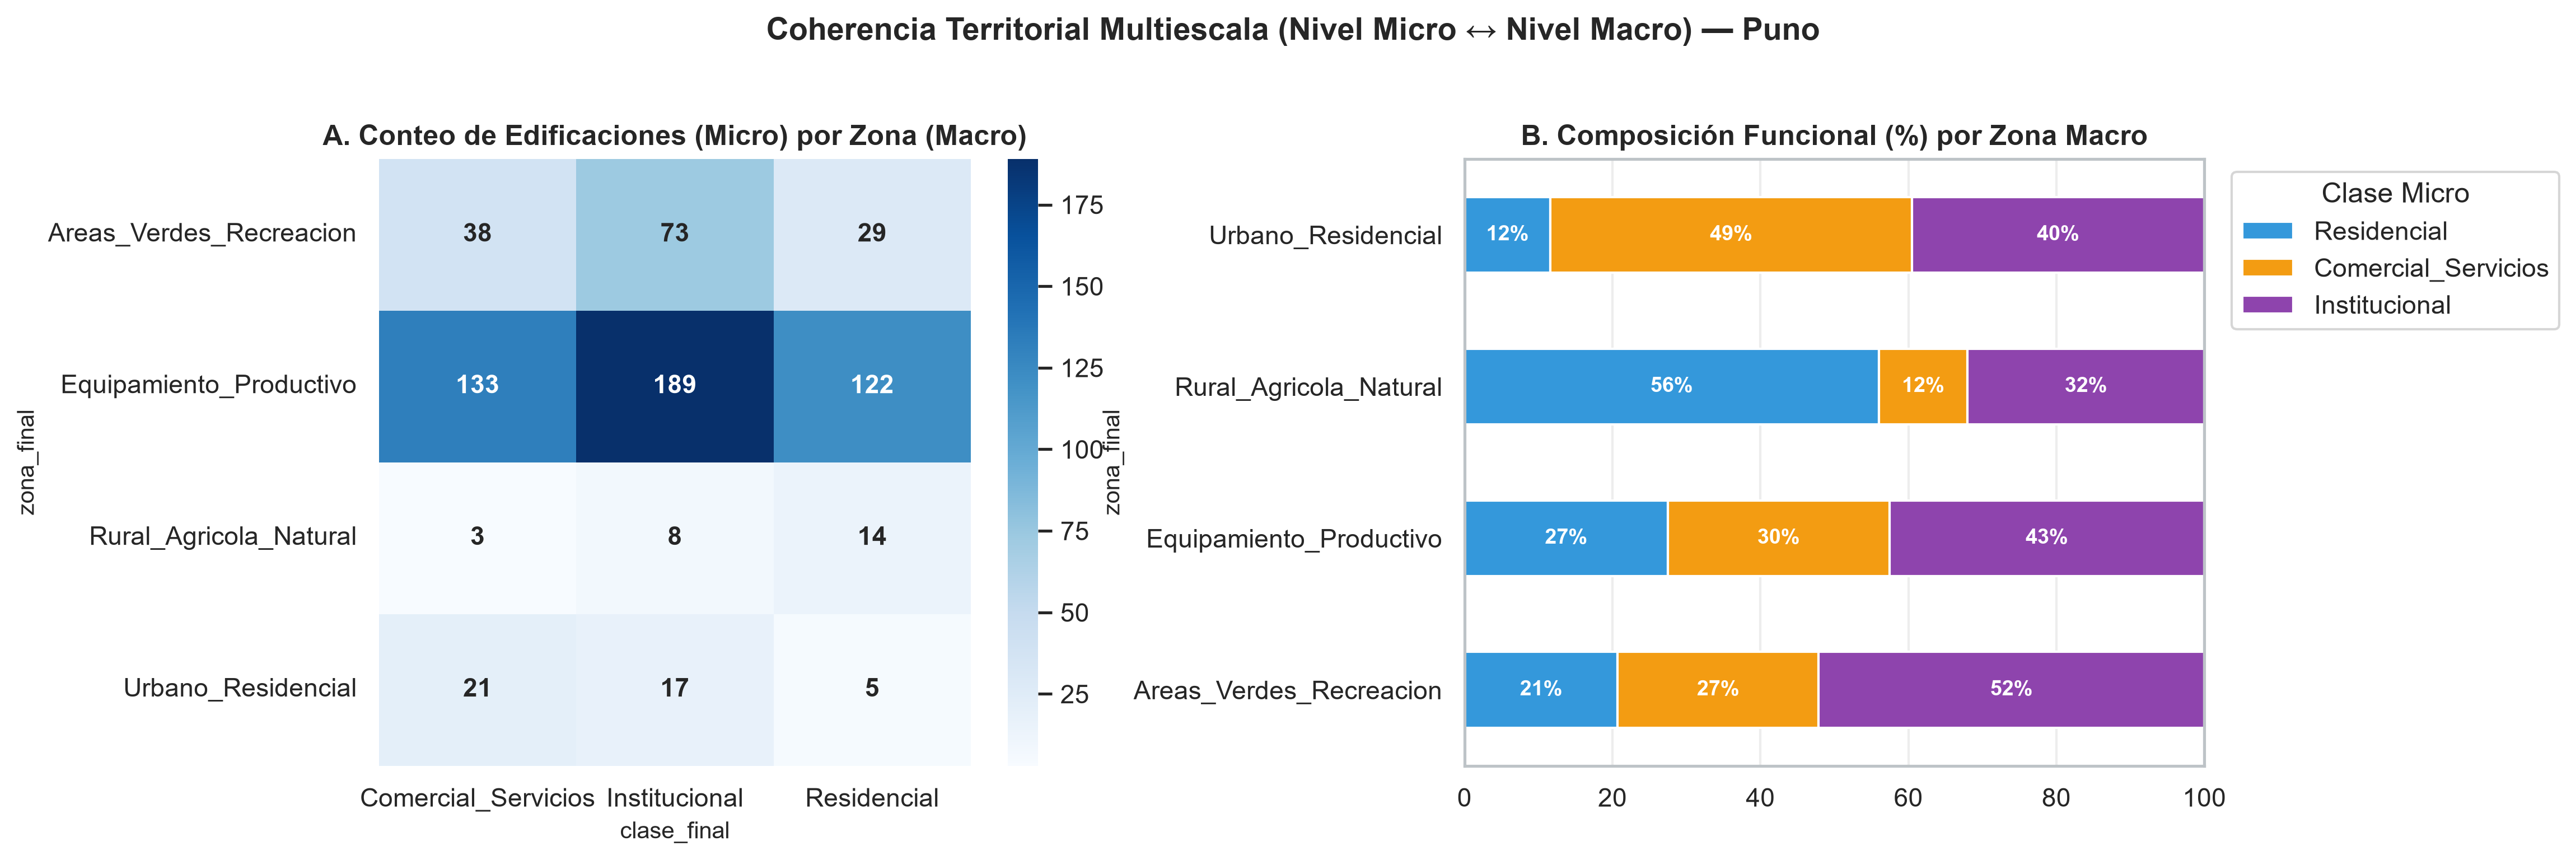
\includegraphics[width=0.98\textwidth]{figures/04_coherencia_multiescala.png}
    \caption{Coherencia territorial multiescala entre las predicciones del Nivel Micro y el Nivel Macro: conteos absolutos por cruce (Panel A) y composición porcentual de usos de edificación en cada zona Macro (Panel B).}
    \label{fig:nb04_coherencia}
\end{figure}

\begin{figure}[H]
    \centering
    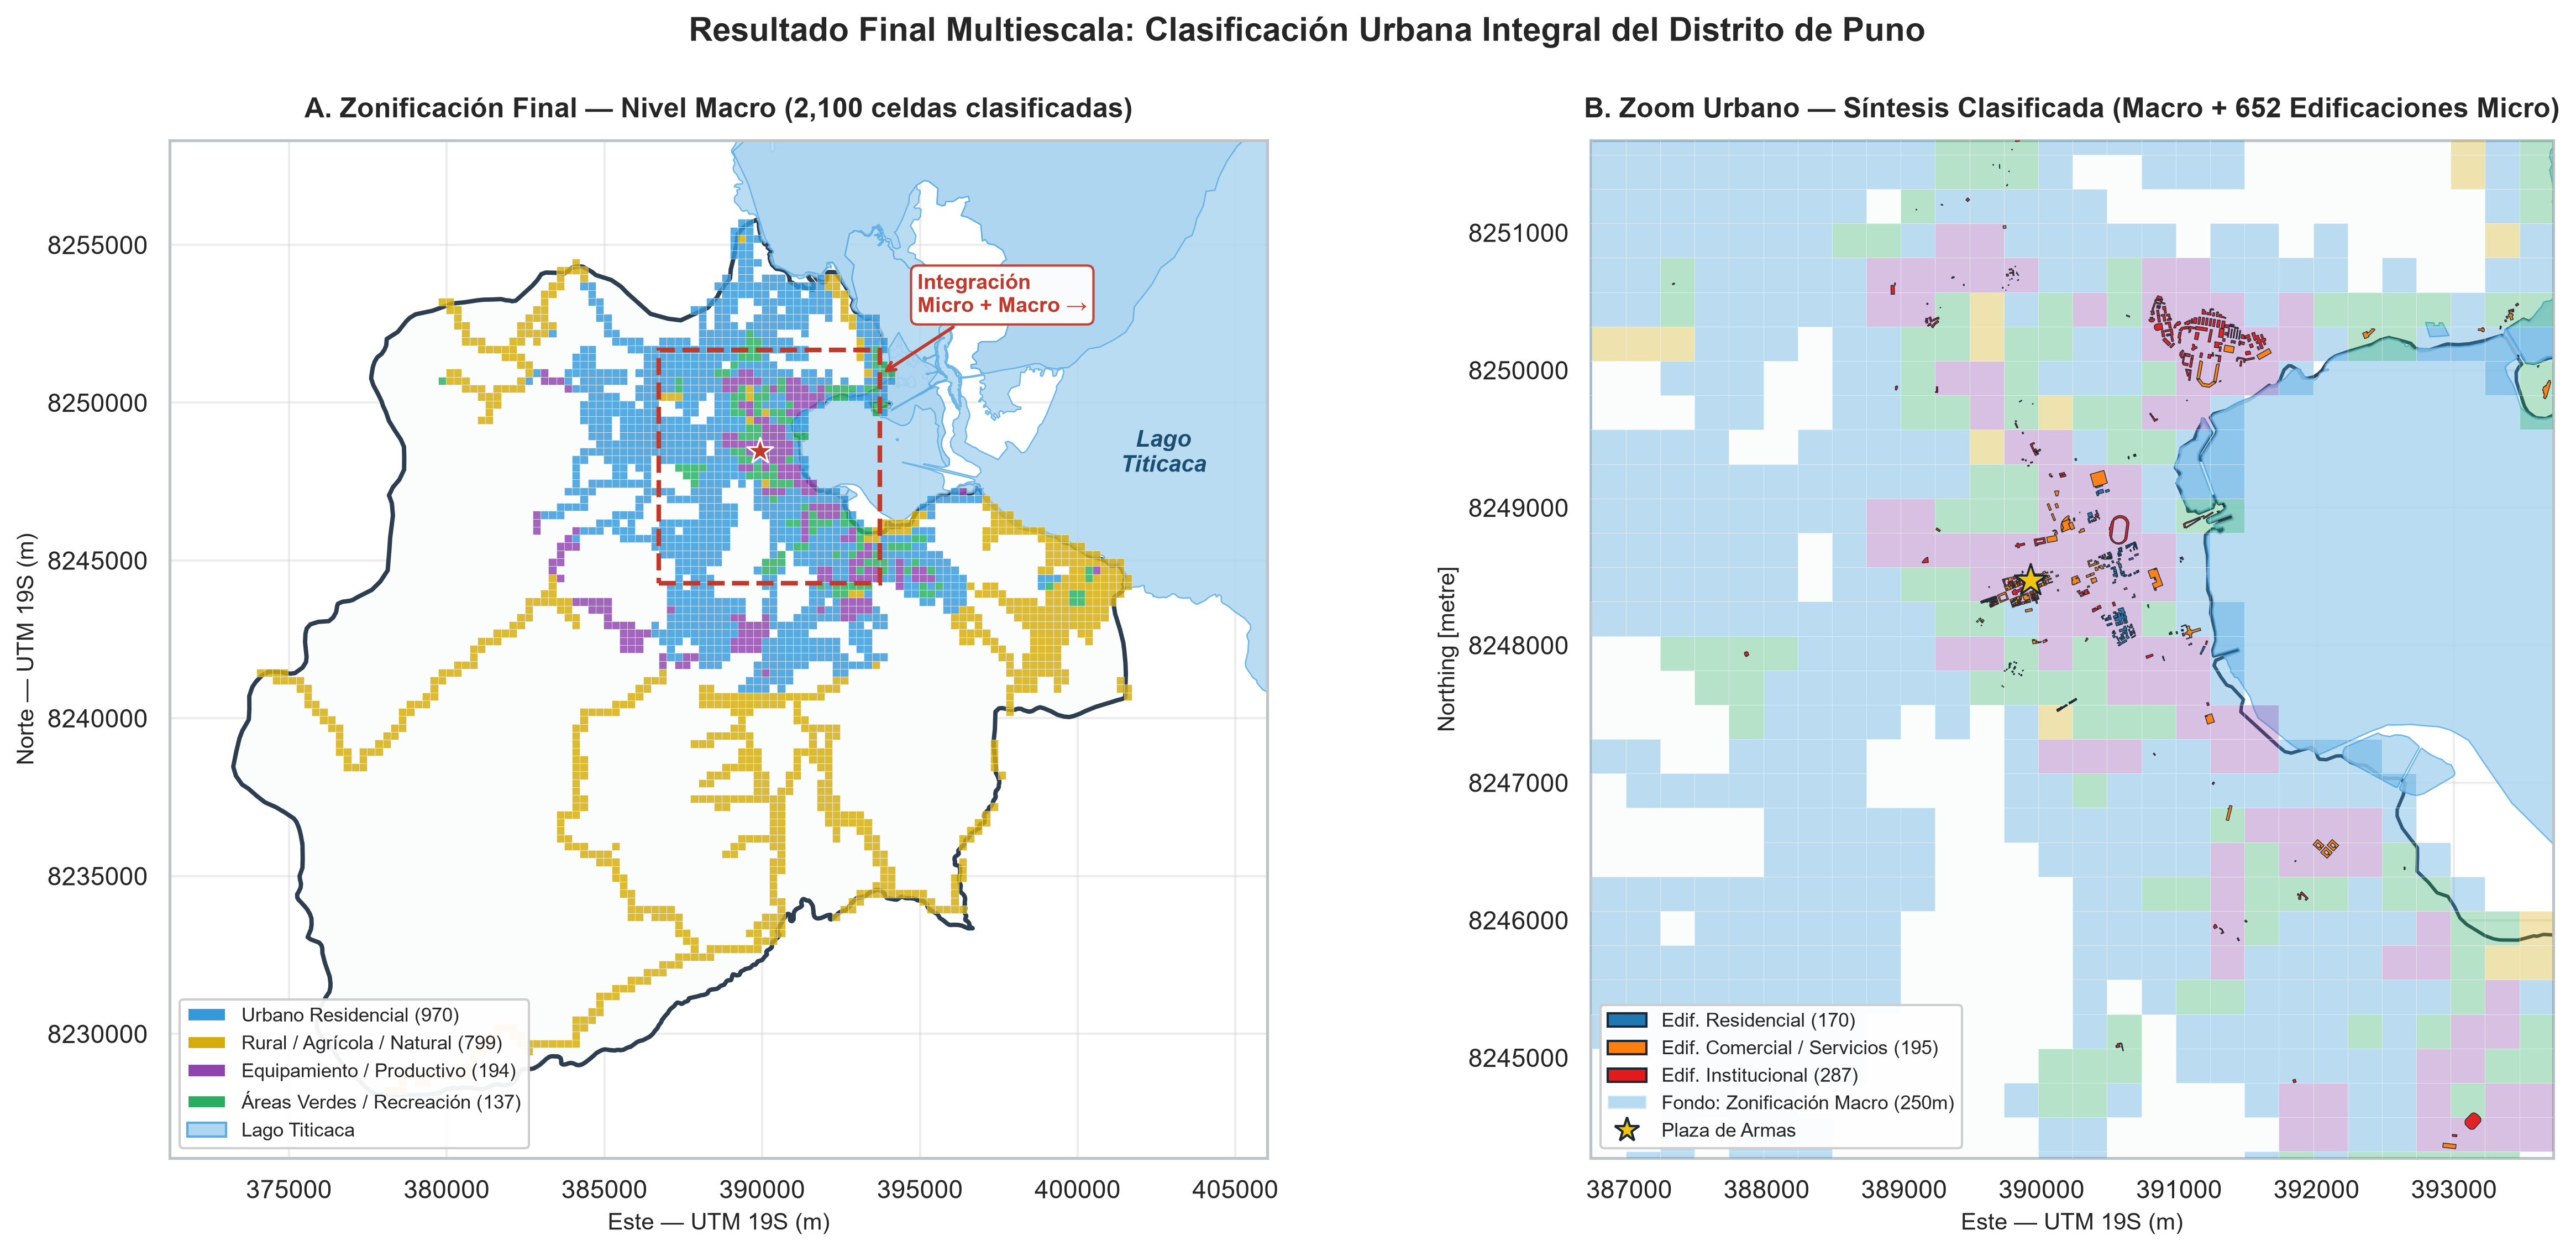
\includegraphics[width=0.98\textwidth]{figures/04_mapa_final_multiescala.png}
    \caption{Síntesis cartográfica final multiescala del Distrito de Puno: zonificación completa de las $2{,}100$ celdas de $250\text{ m} \times 250\text{ m}$ (Panel A) y acercamiento urbano integrando las $652$ edificaciones clasificadas en Nivel Micro sobre la grilla Macro (Panel B).}
    \label{fig:nb04_mapa_final}
\end{figure}

% ==============================================================================
% SECCIÓN 6: CONCLUSIONES, LIMITACIONES Y TRABAJO FUTURO
% ==============================================================================
\newpage

\section{Conclusiones}

\begin{enumerate}[leftmargin=0.8cm, itemsep=3pt]
    \item \textbf{Viabilidad de la clasificación urbana multiescala con datos abiertos:} El recorte optimizado de las capas nacionales de OpenStreetMap hacia el límite oficial del Distrito de Puno ($460.41\text{ km}^2$) en proyección métrica \texttt{EPSG:32719} redujo el volumen de trabajo de $\sim 1.5\text{ GB}$ a $3.53\text{ MB}$ en formato \texttt{GeoJSON}, permitiendo construir un flujo reproducible que clasificó e imputó el $100\%$ de las $652$ edificaciones (Nivel Micro) y de las $2{,}100$ celdas territoriales activas de $250\text{ m} \times 250\text{ m}$ (Nivel Macro).
    \item \textbf{Superioridad consistente de los ensambles frente a los árboles simples:} Los modelos de ensamble superaron a los árboles individuales en ambas escalas al reducir la varianza mediante agregación paralela (\textit{Bagging}) o corrección secuencial de residuos (\textit{Boosting}). En el Nivel Micro, \textbf{LightGBM} lideró la validación cruzada (\texttt{CV-5 F1-Macro} $= 0.7496$ en $63.35\text{ ms}$) y \textbf{Random Forest} encabezó el examen final (\texttt{Test Accuracy} $= 0.8378$, \texttt{F1-Macro} $= 0.8115$). En el Nivel Macro, \textbf{Random Forest} ganó en validación cruzada (\texttt{CV-5 F1-Macro} $= 0.6980$), seguido en empate técnico por \textbf{XGBoost} ($0.6977$), el cual obtuvo el mejor resultado en Test (\texttt{Test Accuracy} $= 0.7772$, \texttt{F1-Macro} $= 0.7120$, \texttt{F1-Weighted} $= 0.7814$).
    \item \textbf{Importancia de las estructuras de datos espaciales (\texttt{cKDTree}) y coherencia territorial:} La ingeniería de variables basada en \texttt{cKDTree} ($O(\log N)$) junto con la morfología geométrica demostró ser determinante para capturar la estructura real de Puno —identificando la superficie construida, la densidad de servicios locales, la accesibilidad vial, la centralidad hacia la Plaza de Armas y la distancia al Lago Titicaca como los principales factores discriminantes—. El consenso unánime de los cuatro paradigmas ($73.0\%$ en Micro y $56.9\%$ en Macro), los elevados índices $\kappa$ de Cohen y el cruce territorial entre escalas corroboran la solidez del sistema propuesto.
\end{enumerate}
\newpage
\section{Limitaciones del Estudio}

Durante el desarrollo e interpretación de los resultados se identificaron cuatro limitaciones principales que acotan el alcance actual del proyecto:
\begin{itemize}[leftmargin=0.8cm, itemsep=2pt]
    \item \textbf{Completitud y sesgo espacial de los datos voluntarios (OSM):} Al provenir de mapeo colaborativo, la capa de edificaciones de Puno contiene únicamente $652$ polígonos digitalizados (concentrados mayoritariamente en el centro histórico y la UNA Puno) y solo $184$ disponen de etiqueta verificable; de forma análoga, el $52.0\%$ de las celdas activas del Nivel Macro carece de etiqueta base de \texttt{landuse}. Esto impide cubrir actualmente las viviendas periféricas aún no trazadas en OSM.
    \item \textbf{Tamaño muestral acotado en el conjunto de prueba Micro ($n=37$):} Si bien la selección del modelo se protegió mediante validación cruzada estratificada de $5$ particiones, un conjunto de prueba de $37$ edificaciones introduce mayor sensibilidad puntual frente a pocos casos atípicos (como grandes hoteles o complejos deportivos).
    \item \textbf{Usos mixtos dentro de celdas cuadradas de $250\text{ m} \times 250\text{ m}$:} En el casco urbano consolidado, una cuadrícula de $6.25\text{ hectáreas}$ engloba frecuentemente viviendas, locales comerciales y parques vecinales de forma simultánea, generando una ambigüedad física inherente que explica las confusiones residuales.
    \item \textbf{Ausencia de información vertical, censal y espectral:} Las geometrías vectoriales bidimensionales de OSM no registran altura de edificaciones, número de pisos, densidad poblacional por manzana ni reflectancia satelital, atributos que ayudarían a diferenciar edificaciones multifamiliares, áreas verdes sin etiquetar y bordes periurbanos en consolidación.
\end{itemize}
\newpage
\section{Trabajos Futuros y Potenciales Mejoras}

A partir de las limitaciones identificadas, se proponen cuatro líneas concretas de mejora para evolucionar el sistema hacia una herramienta operativa de gestión urbana:
\begin{itemize}[leftmargin=0.8cm, itemsep=2pt]
    \item \textbf{Adopción de grillas hexagonales jerárquicas:} Reemplazar la malla cuadrada fija de $250\text{ m}$ por teselaciones hexagonales que aseguren equidistancia con los seis vecinos inmediatos, reduzcan el sesgo de borde y permitan variar la resolución espacial (por ejemplo, celdas más finas en el centro histórico y más amplias en zonas rurales).
    \item \textbf{Validación cruzada espacial:} Complementar la validación estratificada aleatoria con particiones por bloques geográficos contiguos para evaluar con mayor rigor la capacidad de generalización frente a la autocorrelación espacial en sectores de expansión urbana no observados.
\end{itemize}

% ==============================================================================
% REFERENCIAS (FORMATO APA CON SANGRÍA FRANCESA — SELECCIÓN ESENCIAL)
% ==============================================================================
\newpage
\section*{Referencias}
\addcontentsline{toc}{section}{Referencias}

\begingroup
\setlength{\parindent}{0pt}
\setlength{\parskip}{5pt}
\small

\hangindent=1.0cm \hangafter=1
Bentley, J. L. (1975). Multidimensional binary search trees used for associative searching. \textit{Communications of the ACM}, 18(9), 509--517. \url{https://doi.org/10.1145/361002.361007}

\hangindent=1.0cm \hangafter=1
Breiman, L. (2001). Random forests. \textit{Machine Learning}, 45(1), 5--32. \url{https://doi.org/10.1023/A:1010933404324}

\hangindent=1.0cm \hangafter=1
Breiman, L., Friedman, J. H., Olshen, R. A., \& Stone, C. J. (1984). \textit{Classification and regression trees}. Wadsworth International Group.

\hangindent=1.0cm \hangafter=1
Chen, T., \& Guestrin, C. (2016). XGBoost: A scalable tree boosting system. En \textit{Proceedings of the 22nd ACM SIGKDD International Conference on Knowledge Discovery and Data Mining} (pp. 785--794). ACM. \url{https://doi.org/10.1145/2939672.2939785}

\hangindent=1.0cm \hangafter=1
Cohen, J. (1960). A coefficient of agreement for nominal scales. \textit{Educational and Psychological Measurement}, 20(1), 37--46. \url{https://doi.org/10.1177/001316446002000104}

\hangindent=1.0cm \hangafter=1
Haklay, M., \& Weber, P. (2008). OpenStreetMap: User-generated street maps. \textit{IEEE Pervasive Computing}, 7(4), 12--18. \url{https://doi.org/10.1109/MPRV.2008.80}

\hangindent=1.0cm \hangafter=1
Ke, G., Meng, Q., Finley, T., Wang, T., Chen, W., Ma, W., Ye, Q., \& Liu, T.-Y. (2017). LightGBM: A highly efficient gradient boosting decision tree. \textit{Advances in Neural Information Processing Systems}, 30, 3146--3154.

\hangindent=1.0cm \hangafter=1
Quinlan, J. R. (1986). Induction of decision trees. \textit{Machine Learning}, 1(1), 81--106. \url{https://doi.org/10.1007/BF00116251}

\endgroup

\end{document}
